% Options for packages loaded elsewhere
\PassOptionsToPackage{unicode}{hyperref}
\PassOptionsToPackage{hyphens}{url}
%
\documentclass[
]{book}
\usepackage{amsmath,amssymb}
\usepackage{lmodern}
\usepackage{iftex}
\ifPDFTeX
  \usepackage[T1]{fontenc}
  \usepackage[utf8]{inputenc}
  \usepackage{textcomp} % provide euro and other symbols
\else % if luatex or xetex
  \usepackage{unicode-math}
  \defaultfontfeatures{Scale=MatchLowercase}
  \defaultfontfeatures[\rmfamily]{Ligatures=TeX,Scale=1}
\fi
% Use upquote if available, for straight quotes in verbatim environments
\IfFileExists{upquote.sty}{\usepackage{upquote}}{}
\IfFileExists{microtype.sty}{% use microtype if available
  \usepackage[]{microtype}
  \UseMicrotypeSet[protrusion]{basicmath} % disable protrusion for tt fonts
}{}
\makeatletter
\@ifundefined{KOMAClassName}{% if non-KOMA class
  \IfFileExists{parskip.sty}{%
    \usepackage{parskip}
  }{% else
    \setlength{\parindent}{0pt}
    \setlength{\parskip}{6pt plus 2pt minus 1pt}}
}{% if KOMA class
  \KOMAoptions{parskip=half}}
\makeatother
\usepackage{xcolor}
\usepackage{color}
\usepackage{fancyvrb}
\newcommand{\VerbBar}{|}
\newcommand{\VERB}{\Verb[commandchars=\\\{\}]}
\DefineVerbatimEnvironment{Highlighting}{Verbatim}{commandchars=\\\{\}}
% Add ',fontsize=\small' for more characters per line
\usepackage{framed}
\definecolor{shadecolor}{RGB}{248,248,248}
\newenvironment{Shaded}{\begin{snugshade}}{\end{snugshade}}
\newcommand{\AlertTok}[1]{\textcolor[rgb]{0.94,0.16,0.16}{#1}}
\newcommand{\AnnotationTok}[1]{\textcolor[rgb]{0.56,0.35,0.01}{\textbf{\textit{#1}}}}
\newcommand{\AttributeTok}[1]{\textcolor[rgb]{0.77,0.63,0.00}{#1}}
\newcommand{\BaseNTok}[1]{\textcolor[rgb]{0.00,0.00,0.81}{#1}}
\newcommand{\BuiltInTok}[1]{#1}
\newcommand{\CharTok}[1]{\textcolor[rgb]{0.31,0.60,0.02}{#1}}
\newcommand{\CommentTok}[1]{\textcolor[rgb]{0.56,0.35,0.01}{\textit{#1}}}
\newcommand{\CommentVarTok}[1]{\textcolor[rgb]{0.56,0.35,0.01}{\textbf{\textit{#1}}}}
\newcommand{\ConstantTok}[1]{\textcolor[rgb]{0.00,0.00,0.00}{#1}}
\newcommand{\ControlFlowTok}[1]{\textcolor[rgb]{0.13,0.29,0.53}{\textbf{#1}}}
\newcommand{\DataTypeTok}[1]{\textcolor[rgb]{0.13,0.29,0.53}{#1}}
\newcommand{\DecValTok}[1]{\textcolor[rgb]{0.00,0.00,0.81}{#1}}
\newcommand{\DocumentationTok}[1]{\textcolor[rgb]{0.56,0.35,0.01}{\textbf{\textit{#1}}}}
\newcommand{\ErrorTok}[1]{\textcolor[rgb]{0.64,0.00,0.00}{\textbf{#1}}}
\newcommand{\ExtensionTok}[1]{#1}
\newcommand{\FloatTok}[1]{\textcolor[rgb]{0.00,0.00,0.81}{#1}}
\newcommand{\FunctionTok}[1]{\textcolor[rgb]{0.00,0.00,0.00}{#1}}
\newcommand{\ImportTok}[1]{#1}
\newcommand{\InformationTok}[1]{\textcolor[rgb]{0.56,0.35,0.01}{\textbf{\textit{#1}}}}
\newcommand{\KeywordTok}[1]{\textcolor[rgb]{0.13,0.29,0.53}{\textbf{#1}}}
\newcommand{\NormalTok}[1]{#1}
\newcommand{\OperatorTok}[1]{\textcolor[rgb]{0.81,0.36,0.00}{\textbf{#1}}}
\newcommand{\OtherTok}[1]{\textcolor[rgb]{0.56,0.35,0.01}{#1}}
\newcommand{\PreprocessorTok}[1]{\textcolor[rgb]{0.56,0.35,0.01}{\textit{#1}}}
\newcommand{\RegionMarkerTok}[1]{#1}
\newcommand{\SpecialCharTok}[1]{\textcolor[rgb]{0.00,0.00,0.00}{#1}}
\newcommand{\SpecialStringTok}[1]{\textcolor[rgb]{0.31,0.60,0.02}{#1}}
\newcommand{\StringTok}[1]{\textcolor[rgb]{0.31,0.60,0.02}{#1}}
\newcommand{\VariableTok}[1]{\textcolor[rgb]{0.00,0.00,0.00}{#1}}
\newcommand{\VerbatimStringTok}[1]{\textcolor[rgb]{0.31,0.60,0.02}{#1}}
\newcommand{\WarningTok}[1]{\textcolor[rgb]{0.56,0.35,0.01}{\textbf{\textit{#1}}}}
\usepackage{longtable,booktabs,array}
\usepackage{calc} % for calculating minipage widths
% Correct order of tables after \paragraph or \subparagraph
\usepackage{etoolbox}
\makeatletter
\patchcmd\longtable{\par}{\if@noskipsec\mbox{}\fi\par}{}{}
\makeatother
% Allow footnotes in longtable head/foot
\IfFileExists{footnotehyper.sty}{\usepackage{footnotehyper}}{\usepackage{footnote}}
\makesavenoteenv{longtable}
\usepackage{graphicx}
\makeatletter
\def\maxwidth{\ifdim\Gin@nat@width>\linewidth\linewidth\else\Gin@nat@width\fi}
\def\maxheight{\ifdim\Gin@nat@height>\textheight\textheight\else\Gin@nat@height\fi}
\makeatother
% Scale images if necessary, so that they will not overflow the page
% margins by default, and it is still possible to overwrite the defaults
% using explicit options in \includegraphics[width, height, ...]{}
\setkeys{Gin}{width=\maxwidth,height=\maxheight,keepaspectratio}
% Set default figure placement to htbp
\makeatletter
\def\fps@figure{htbp}
\makeatother
\setlength{\emergencystretch}{3em} % prevent overfull lines
\providecommand{\tightlist}{%
  \setlength{\itemsep}{0pt}\setlength{\parskip}{0pt}}
\setcounter{secnumdepth}{5}
\usepackage{booktabs}
\ifLuaTeX
  \usepackage{selnolig}  % disable illegal ligatures
\fi
\usepackage[]{natbib}
\bibliographystyle{plainnat}
\IfFileExists{bookmark.sty}{\usepackage{bookmark}}{\usepackage{hyperref}}
\IfFileExists{xurl.sty}{\usepackage{xurl}}{} % add URL line breaks if available
\urlstyle{same} % disable monospaced font for URLs
\hypersetup{
  pdftitle={Machine Learning for Economics and Business},
  pdfauthor={Zijun Luo},
  hidelinks,
  pdfcreator={LaTeX via pandoc}}

\title{Machine Learning for Economics and Business}
\author{Zijun Luo}
\date{2023-06-25}

\usepackage{amsthm}
\newtheorem{theorem}{Theorem}[chapter]
\newtheorem{lemma}{Lemma}[chapter]
\newtheorem{corollary}{Corollary}[chapter]
\newtheorem{proposition}{Proposition}[chapter]
\newtheorem{conjecture}{Conjecture}[chapter]
\theoremstyle{definition}
\newtheorem{definition}{Definition}[chapter]
\theoremstyle{definition}
\newtheorem{example}{Example}[chapter]
\theoremstyle{definition}
\newtheorem{exercise}{Exercise}[chapter]
\theoremstyle{definition}
\newtheorem{hypothesis}{Hypothesis}[chapter]
\theoremstyle{remark}
\newtheorem*{remark}{Remark}
\newtheorem*{solution}{Solution}
\begin{document}
\maketitle

{
\setcounter{tocdepth}{1}
\tableofcontents
}
\hypertarget{preface}{%
\chapter*{Preface}\label{preface}}
\addcontentsline{toc}{chapter}{Preface}

The primary purpose of these articles, which I started to write in May 2023, is to review, summarize, and organize what I have learned in Machine Learning as a PhD economist. I have taken several Machine Learning related courses on Coursera and Udemy. In 2022, I also worked, briefly, as a data scientist in an AdTech start-up.

In my mind, I pretend that these articles are written for those who have some quantitative training but is interested in what Machine Learning can offer, particularly graduate students who have taken at least one econometrics course. My emphases are those algorithms that can provide an alternative, sometimes more useful and rigorous, approach to known problems in economics, business, and social sciences. I also provide Python scripts that I have written to implement these algorithms.

\hypertarget{randomized-controlled-trial-abn-testing-and-multi-armed-bandit-algorithms}{%
\chapter{Randomized Controlled Trial, A/B/N Testing, and Multi-Armed Bandit Algorithms}\label{randomized-controlled-trial-abn-testing-and-multi-armed-bandit-algorithms}}

\hypertarget{introduction}{%
\section{Introduction}\label{introduction}}

Randomized Controlled Trial (RCT) is the gold standard for establishing causality in experimental methods. It is used widely in clinical trials for new drugs or field experiments in social sciences and economics. In business, especially e-commerce, a related concept is A/B/N Testing. The main idea of RCT and A/B/N test is straightforward: individuals are randomly divided into groups to receive different treatments. Afterwards treatments, outcomes are being valuated and compared in order to find out which treatment works better/best. In RCT, a control group, where individuals receive a ``placebo'', is usually included. Note that placebo should be considered as a type of treatment too and individuals who receive a placebo are not getting ``nothing''. A placebo is something that has no therapeutic effect, i.e., it is not designed to cure a disease or an illness. But it can nevertheless positively impact the well-being of individuals who have received it, if due to nothing but psychological effects. As a result, it would be rather wrong to expect ``no effect'' from the the controlled group that receives the placebo in an RCT.

In the rest of this article, I will be using A/B/N test as the example because I want to stay away from the nitty-gritty details of RCT. I am using ``A/B/N'' to include tests with more than 2 versions. If you are only comparing two versions, it is an A/B test.

When I was interviewing for a data scientist job in 2022, the following was one of the interview questions: We are going to run an A/B test on a client's website. How long do we need to run the experiment for? Back then I knew about how to find minimum sample size based on hypothesis testing in Statistics, so I framed my answer that way. But I stopped in the middle while answering the question. Something I did not think seriously enough about popped into my head: how would I know the standard deviation, one of the required values to carry out the calculation for minimum sample size, before we even run the experiment? My interview went downhill from there. Needless to say, I did not get the job. However, the interviewer was nice enough to tell me that I should look into ``power analysis''.

I did. Suppose you have built an e-commerce website with two possible color pallettes, and you want to understand which color pallette would induce more purchases. You can randomly assign a visitor to the two versions of the website, and after a while, you will have a dataset with two columns: for each visitor, you recorded the version that the visitor was assigned to and the purchases that the visitor made. For \(i\in(A,B)\), let's define the following values:
* \(\bar{x}_i\): expected dollars spent by visitors of version \(i\);
* \(n_i\): number of visitors who saw version \(i\);
* \(s_i\): standard deviation of dollars spent by visitors who saw version \(i\).

We can now calculate the ``power'' as
\[t=\frac{\bar{x}_A-\bar{x}_B}{s_p\sqrt{\tfrac{1}{n_A}+\tfrac{1}{n_B}}}\]
where \(s_p=\sqrt{\frac{(n_A-1)s_A^2+(n_B-1)s_B^2}{n_A+n_B-2}}\) is the pooled standard deviation. The ``power'', \(t\), follows a \(t\)-distribution with \(n_A+n_B-2\) degrees of freedom.

Suppose \(s_A=s_B\) for the two versions in your A/B test, we can denote the two standard deviations as \(s\). Also suppose, for simplicity, you want \(n_A=n_B\). You can solve for \(n_i\) from the above power analysis formula and obtain:
\[N=\frac{4t^2s^2}{(\bar{x}_A-\bar{x}_B)^2}\]
where \(N\) is the total sample size (\(n_A+n_B\)). It is easy to see that you will need a larger sample size if
* the expected difference between the two versions are smaller;
* you want a better significance level, e.g., 1\% instead of 5\%;
* the standard deviation is bigger, i.e., dollars spent are more dispersed among individuals;

But here is the problem: you do not know the values of \(\bar{x}_i\) and \(s_i\) before the experiment. For \(\bar{x}_i\), it may be less of an issue. Instead of the expected values, all you really need is the \emph{expected difference}, which can be specified. For example, suppose your website is currently running Version A, and all you care about is that Version B can increase expected purchase amount by 15. In other words, \(\bar{x}_B-\bar{x}_A=15\). But you still need to know the standard deviations. How? Some suggest that you can run a short trial to estimate the standard deviation. But then, isn't the A/B test already a trial itself?

Here is another problem about classic A/B test design. After I became a data scientist, at another company, we actually ran an A/B test. The problem is that, according to the aforementioned power analysis, the experiment needed to be ran for at least 3 months, but we did not have that much time. After 1 month, our model (Version B) outperformed the existed model (Version A). Could we have declared our model to be the better one? According to classic A/B test design, the answer is ``No'' because we should not be ``peeking'' as the difference can be driven by random factors happened only in the first month of the experiment.

Now think about clinical trials for a new drug, where the ``no peeking'' rule can raise serious concerns. If a drug has proved its effectiveness in the first 500 patients, yet the power analysis tells you that you need to test it on 50,000 patients, what would you do? Isn't it unethical to continue to give a placebo to individuals who may benefit from the actual drug?

These two problems have bothered me for a while, until I learned about the approaches I will cover in this article. Here is a brief overview of how these algorithms work. Instead of having a predetermined sample size, the A/B test is deployed in real-time. Continued with our example of a website with two color pallettes, a visitor is randomly assigned to a version of the website on the first visit. An algorithm will then pick a version for a visitor. In general, the version that has received higher purchase values should get more visitors. But how do we know which one gives the higher payoff? Here, we face the Explore-Exploit Tradeoff.

\hypertarget{the-explore-exploit-tradeoff}{%
\section{The Explore-Exploit Tradeoff}\label{the-explore-exploit-tradeoff}}

In a nutshell, the explore-exploit tradeoff shows the following paradox: in order to find the best version, you need to explore, which means that the outcome of exploration necessarily improves the more you different versions. However, to maximize total payoff, you want to stick with the best version once (you think) you have found it, which is to exploit. This means that the outcome of exploitation necessarily deteriorates the more you different versions since there is one and only one best version.

How to handle the explore-exploit tradeoff constitutes the core difference among algorithms. Some algorithms, such as variants of the ``greedy'' family, really focuses on exploitation. The disadvantage is that such algorithm can easily ``saddle'' into the second-best as long as the second-best is ``good enough'', as I will show later when we discuss the \texttt{Epsilon\ Greedy} algorithm. Others, such as \texttt{Upper\ Confidence\ Bound}, put more emphasis on exploration, at least initially.

If you are reading this article because you think it may help you with your research project(s), you are not a stranger to the explore-exploit tradeoff. I remember a conversation I had with a professor not long after I graduated. I asked him if I should have given up on projects that I do not think that would end up in good journals. His answer was: but how do you know before you try? He had a point: my professor never published his PhD dissertation. He was successful after he has explored a new area of research. However, about 15 years after his dissertation, a paper on a closely related topic was published in a top journal. In retrospect, he may have explored more than the optimum, which was probably why he suggested me to exploit more.

\hypertarget{epsilon-greedy}{%
\section{Epsilon Greedy}\label{epsilon-greedy}}

We will begin our in-depth discussion of algorithms with \texttt{Epsilon\ Greedy}. For each algorithm, I aim to provide:
* intuition and description of theory
* pseudocode
* \texttt{Python} code

Algorithms in the \texttt{Greedy} family applies a simple logic: choose the version that gives the best \emph{observed} expected payoff. For simplicity, and for the rest of this article, let's consider an e-commerce website that has 5 different designs but sells a single product: an EveryDay-Carry (EDC) musical instrument for 69.99 dollars. If we run an A/B/N test on the web designs, only 2 outcomes are possible from each visitor: buy or not buy.

Here is the pseudocode for a simple \texttt{Greedy} algorithm:

\begin{verbatim}
loop:
    j = argmax(expected bandit win rates)
    x = reward (1 or 0) from playing bandit j
    bandit[j].update_mean(x)
\end{verbatim}

I used \textbf{bandit} instead of \textbf{version} here, and will be using these two terms interchangeably, because the problem we are working on is commonly known as the \texttt{Multi-Armed\ Bandits} problem in probability theory and reinforcement learning. The analogy comes from choosing among multiple slot machines in a casino since a single slot machine is referred to as a ``one-armed bandit''.

Let's take a closer look at the pseudocode. In this pseudocode, \(i\) indexes visitor, \(j\) indexes the website version (or bandit), and \(x\) is 1 when the visitor buys and 0 otherwise. Furthermore, \texttt{update\_mean()} is a function that takes the new value of \texttt{x} and updates the expected payoff for bandit \texttt{j}. To update the expected payoff after bandit \texttt{j} was played for the \(n_{th}\) time, we have

\[\bar{x}_n=\bar{x}_{n-1}+\frac{x_n-\bar{x}_{n-1}}{n}\]

This calculates the mean in \emph{constant time and memory}, i.e., it requires only 3 values to calculate the mean, \(\bar{x}_n\), regardless of the value of \(n\): \(\bar{x}_{n-1}\), \(x_n\), and \(n\), whereas the number of values required to calculate the mean with the formula

\[\bar{x}_n=\frac{\sum_{i=1}^n{x_i}}{n}\]

increases with \(n\).

While not necessary, it can sometimes be a good idea to try all versions in the beginning. For example, for the first 50 visitors, we can send them to each design with equal probability. From that point on, the algorithm finds the version that gives the best expected payoff, and play that version.

It should be obvious that the simple \texttt{Greedy} algorithm has a problem: once it finds a bandit with a \emph{high enough} payoff, it rarely switches. In other words, it almost never explores. The \texttt{Epsilon\ Greedy} algorithm provides a simple fix:

\begin{verbatim}
loop:
    p = random number in [0, 1]
    if p < epsilon:
        j = choose a bandit at random
    else:
        j = argmax(expected bandit win rates)
    x = reward (1 or 0) from playing bandit j
    bandit[j].update_mean(x)
\end{verbatim}

As the pseudocode shows, a random value is drawn when a new visitor has arrived. If the random value is smaller than the threshold, \texttt{epsilon}, set before the start of the experiment, then a random bandit is picked. Note that this randomly picked bandit can be the same as the one picked by \texttt{argmax}. To exclude such case only requires a few more lines of code. However, this is not a requirement of the \texttt{Epsilon\ Greedy} algorithm and the benefit of doing so is not obvious.

Let's now move onto the actual implementation of \texttt{Epsilon\ Greedy} in \texttt{Python}. Note that the script includes lines with the comment ``\emph{only in demonstration}''. These are codes to generate the \emph{true} win rate of different bandits, which you do not know when running a real-world experiment. This also means you can not use the scripts here in real-world problems without making necessary changes.

\begin{Shaded}
\begin{Highlighting}[]
\ImportTok{import}\NormalTok{ numpy }\ImportTok{as}\NormalTok{ np}
\ImportTok{import}\NormalTok{ random}

\CommentTok{\# set the number of bandits}
\NormalTok{N\_bandits }\OperatorTok{=} \DecValTok{5}
\CommentTok{\# set the number of trials}
\CommentTok{\# only in demonstration}
\NormalTok{N }\OperatorTok{=} \DecValTok{100000}


\KeywordTok{class}\NormalTok{ BayesianAB:}
    \KeywordTok{def} \FunctionTok{\_\_init\_\_}\NormalTok{(}
            \VariableTok{self}\NormalTok{,}
\NormalTok{            number\_of\_bandits: }\BuiltInTok{int} \OperatorTok{=} \DecValTok{2}\NormalTok{,}
\NormalTok{            number\_of\_trials: }\BuiltInTok{int} \OperatorTok{=} \DecValTok{100000}\NormalTok{,}
\NormalTok{            p\_max: }\BuiltInTok{float} \OperatorTok{=} \FloatTok{.75}\NormalTok{,}
\NormalTok{            p\_diff: }\BuiltInTok{float} \OperatorTok{=} \FloatTok{.05}\NormalTok{,}
\NormalTok{            p\_min: }\BuiltInTok{float} \OperatorTok{=} \FloatTok{.1}
\NormalTok{    ):}
        \ControlFlowTok{if}\NormalTok{ p\_min }\OperatorTok{\textgreater{}}\NormalTok{ p\_max }\OperatorTok{{-}}\NormalTok{ p\_diff:}
            \ControlFlowTok{raise} \PreprocessorTok{ValueError}\NormalTok{(}\StringTok{"Condition p\_min \textless{} p\_max {-} p\_diff not satisfied. Exit..."}\NormalTok{)}

        \VariableTok{self}\NormalTok{.prob\_true }\OperatorTok{=}\NormalTok{ [}\DecValTok{0}\NormalTok{] }\OperatorTok{*}\NormalTok{ number\_of\_bandits  }\CommentTok{\# only in demonstration}
        \VariableTok{self}\NormalTok{.prob\_win }\OperatorTok{=}\NormalTok{ [}\DecValTok{0}\NormalTok{] }\OperatorTok{*}\NormalTok{ number\_of\_bandits}
        \VariableTok{self}\NormalTok{.history }\OperatorTok{=}\NormalTok{ []}
        \VariableTok{self}\NormalTok{.history\_bandit }\OperatorTok{=}\NormalTok{ []  }\CommentTok{\# for Monte Carlo}
        \VariableTok{self}\NormalTok{.count }\OperatorTok{=}\NormalTok{ [}\DecValTok{0}\NormalTok{] }\OperatorTok{*}\NormalTok{ number\_of\_bandits  }\CommentTok{\# only in demonstration}
        \CommentTok{\# preference and pi are for gradient\_bandit only}
        \VariableTok{self}\NormalTok{.pref }\OperatorTok{=}\NormalTok{ [}\DecValTok{0}\NormalTok{] }\OperatorTok{*}\NormalTok{ number\_of\_bandits}
        \VariableTok{self}\NormalTok{.pi }\OperatorTok{=}\NormalTok{ [}\DecValTok{1} \OperatorTok{/}\NormalTok{ number\_of\_bandits] }\OperatorTok{*}\NormalTok{ number\_of\_bandits}
        \CommentTok{\# a and b are for bayesian\_bandits only}
        \VariableTok{self}\NormalTok{.alpha }\OperatorTok{=}\NormalTok{ [}\DecValTok{1}\NormalTok{] }\OperatorTok{*}\NormalTok{ number\_of\_bandits}
        \VariableTok{self}\NormalTok{.beta }\OperatorTok{=}\NormalTok{ [}\DecValTok{1}\NormalTok{] }\OperatorTok{*}\NormalTok{ number\_of\_bandits}
        \CommentTok{\# number of trials/visitors}
        \VariableTok{self}\NormalTok{.N }\OperatorTok{=}\NormalTok{ number\_of\_trials}

        \CommentTok{\# set the last bandit to have a win rate of 0.75 and the rest lower}
        \CommentTok{\# only in demonstration}
        \VariableTok{self}\NormalTok{.prob\_true[}\OperatorTok{{-}}\DecValTok{1}\NormalTok{] }\OperatorTok{=}\NormalTok{ p\_max}
        \ControlFlowTok{for}\NormalTok{ i }\KeywordTok{in} \BuiltInTok{range}\NormalTok{(}\DecValTok{0}\NormalTok{, number\_of\_bandits }\OperatorTok{{-}} \DecValTok{1}\NormalTok{):}
            \VariableTok{self}\NormalTok{.prob\_true[i] }\OperatorTok{=} \BuiltInTok{round}\NormalTok{(p\_max }\OperatorTok{{-}}\NormalTok{ random.uniform(p\_diff, p\_max }\OperatorTok{{-}}\NormalTok{ p\_min), }\DecValTok{2}\NormalTok{)}

    \CommentTok{\# Receives a random value of 0 or 1}
    \CommentTok{\# only in demonstration}
    \KeywordTok{def}\NormalTok{ pull(}
            \VariableTok{self}\NormalTok{,}
\NormalTok{            i,}
\NormalTok{    ) }\OperatorTok{{-}\textgreater{}} \BuiltInTok{bool}\NormalTok{:}
        \ControlFlowTok{return}\NormalTok{ random.random() }\OperatorTok{\textless{}} \VariableTok{self}\NormalTok{.prob\_true[i]}

    \CommentTok{\# Updates the mean}
    \KeywordTok{def}\NormalTok{ update(}
            \VariableTok{self}\NormalTok{,}
\NormalTok{            i,}
\NormalTok{            k,}
\NormalTok{    ) }\OperatorTok{{-}\textgreater{}} \VariableTok{None}\NormalTok{:}
\NormalTok{        outcome }\OperatorTok{=} \VariableTok{self}\NormalTok{.pull(i)}
        \CommentTok{\# may use a constant discount rate to discount past}
        \VariableTok{self}\NormalTok{.prob\_win[i] }\OperatorTok{=}\NormalTok{ (}\VariableTok{self}\NormalTok{.prob\_win[i] }\OperatorTok{*}\NormalTok{ k }\OperatorTok{+}\NormalTok{ outcome) }\OperatorTok{/}\NormalTok{ (k }\OperatorTok{+} \DecValTok{1}\NormalTok{)}
        \VariableTok{self}\NormalTok{.history.append(}\VariableTok{self}\NormalTok{.prob\_win.copy())}
        \VariableTok{self}\NormalTok{.history\_bandit.append(i)  }\CommentTok{\# for Monte Carlo}
        \VariableTok{self}\NormalTok{.count[i] }\OperatorTok{+=} \DecValTok{1}

    \CommentTok{\#\#\#\#\#\#\#\#\#\#\#\#\#\#\#\#\#\#\#\#}
    \CommentTok{\# epsilon greedy}
    \KeywordTok{def}\NormalTok{ epsilon\_greedy(}
            \VariableTok{self}\NormalTok{,}
\NormalTok{            epsilon: }\BuiltInTok{float} \OperatorTok{=} \FloatTok{0.5}\NormalTok{,}
\NormalTok{    ):}

        \VariableTok{self}\NormalTok{.history.append(}\VariableTok{self}\NormalTok{.prob\_win.copy())}

        \ControlFlowTok{for}\NormalTok{ k }\KeywordTok{in} \BuiltInTok{range}\NormalTok{(}\DecValTok{1}\NormalTok{, }\VariableTok{self}\NormalTok{.N):}
            \ControlFlowTok{if}\NormalTok{ random.random() }\OperatorTok{\textless{}}\NormalTok{ epsilon:}
\NormalTok{                i }\OperatorTok{=}\NormalTok{ random.randrange(}\DecValTok{0}\NormalTok{, }\BuiltInTok{len}\NormalTok{(}\VariableTok{self}\NormalTok{.prob\_win))}
            \ControlFlowTok{else}\NormalTok{:}
\NormalTok{                i }\OperatorTok{=}\NormalTok{ np.argmax(}\VariableTok{self}\NormalTok{.prob\_win)}

            \VariableTok{self}\NormalTok{.update(i, k)}

        \ControlFlowTok{return} \VariableTok{self}\NormalTok{.history}
\end{Highlighting}
\end{Shaded}

Let's break it down. First, we import two libraries: \texttt{numpy} and \texttt{random}. We will be using functions from these libraries such as \texttt{argmax()} from \texttt{numpy} and \texttt{randrange()} from \texttt{random}:

\begin{Shaded}
\begin{Highlighting}[]
\ImportTok{import}\NormalTok{ numpy }\ImportTok{as}\NormalTok{ np}
\ImportTok{import}\NormalTok{ random}
\end{Highlighting}
\end{Shaded}

We then set three global parameters:

\begin{Shaded}
\begin{Highlighting}[]
\CommentTok{\# set the number of bandits}
\NormalTok{N\_bandits }\OperatorTok{=} \DecValTok{5}
\CommentTok{\# set the number of trials/visitors}
\NormalTok{N }\OperatorTok{=} \DecValTok{100000}
\end{Highlighting}
\end{Shaded}

In practice, the value of \texttt{N\_bandits} depends on the number of versions your experiment is set out to test, and the number of visitors, \texttt{N}, is unknown.

In this script, we are creating a class named \texttt{BayesianAB}, and put all the algorithms we cover in this article under \texttt{BayesianAB}. We initiate the class with the following values:

\begin{Shaded}
\begin{Highlighting}[]
\KeywordTok{class}\NormalTok{ BayesianAB:}
    \KeywordTok{def} \FunctionTok{\_\_init\_\_}\NormalTok{(}
            \VariableTok{self}\NormalTok{,}
\NormalTok{            number\_of\_bandits: }\BuiltInTok{int} \OperatorTok{=} \DecValTok{2}\NormalTok{,}
\NormalTok{            number\_of\_trials: }\BuiltInTok{int} \OperatorTok{=} \DecValTok{100000}\NormalTok{,}
\NormalTok{            p\_max: }\BuiltInTok{float} \OperatorTok{=} \FloatTok{.75}\NormalTok{,}
\NormalTok{            p\_diff: }\BuiltInTok{float} \OperatorTok{=} \FloatTok{.05}\NormalTok{,}
\NormalTok{            p\_min: }\BuiltInTok{float} \OperatorTok{=} \FloatTok{.8}
\NormalTok{    ):}
        \ControlFlowTok{if}\NormalTok{ p\_min }\OperatorTok{\textgreater{}}\NormalTok{ p\_max }\OperatorTok{{-}}\NormalTok{ p\_diff:}
            \ControlFlowTok{raise} \PreprocessorTok{ValueError}\NormalTok{(}\StringTok{"Condition p\_min \textless{} p\_max {-} p\_diff not satisfied. Exit..."}\NormalTok{)}

        \VariableTok{self}\NormalTok{.prob\_true }\OperatorTok{=}\NormalTok{ [}\DecValTok{0}\NormalTok{] }\OperatorTok{*}\NormalTok{ number\_of\_bandits  }\CommentTok{\# only in demonstration}
        \VariableTok{self}\NormalTok{.prob\_win }\OperatorTok{=}\NormalTok{ [}\DecValTok{0}\NormalTok{] }\OperatorTok{*}\NormalTok{ number\_of\_bandits}
        \VariableTok{self}\NormalTok{.history }\OperatorTok{=}\NormalTok{ []}
        \VariableTok{self}\NormalTok{.history\_bandit }\OperatorTok{=}\NormalTok{ []  }\CommentTok{\# for Monte Carlo}
        \VariableTok{self}\NormalTok{.count }\OperatorTok{=}\NormalTok{ [}\DecValTok{0}\NormalTok{] }\OperatorTok{*}\NormalTok{ number\_of\_bandits  }\CommentTok{\# only in demonstration}
        \CommentTok{\# preference and pi are for gradient\_bandit only}
        \VariableTok{self}\NormalTok{.pref }\OperatorTok{=}\NormalTok{ [}\DecValTok{0}\NormalTok{] }\OperatorTok{*}\NormalTok{ number\_of\_bandits}
        \VariableTok{self}\NormalTok{.pi }\OperatorTok{=}\NormalTok{ [}\DecValTok{1} \OperatorTok{/}\NormalTok{ number\_of\_bandits] }\OperatorTok{*}\NormalTok{ number\_of\_bandits}
        \CommentTok{\# a and b are for bayesian\_bandits only}
        \VariableTok{self}\NormalTok{.alpha }\OperatorTok{=}\NormalTok{ [}\DecValTok{1}\NormalTok{] }\OperatorTok{*}\NormalTok{ number\_of\_bandits}
        \VariableTok{self}\NormalTok{.beta }\OperatorTok{=}\NormalTok{ [}\DecValTok{1}\NormalTok{] }\OperatorTok{*}\NormalTok{ number\_of\_bandits}
        \CommentTok{\# number of trials/visitors}
        \VariableTok{self}\NormalTok{.N }\OperatorTok{=}\NormalTok{ number\_of\_trials}
\end{Highlighting}
\end{Shaded}

The \texttt{BayesianAB} class accepts 5 parameters:
* \texttt{number\_of\_bandits} has a default value of 2;
* \texttt{number\_of\_trials} indicates the number of rounds/visitors, which has a default value of 100,000;
* \texttt{p\_max} is the highest win rate;
* \texttt{p\_diff} is the smallest possible difference between the highest win rate and the second highest win rate;
* \texttt{p\_min} is the lowest possible win rate, andt the condition \texttt{p\_min\ \textgreater{}\ p\_max\ -\ p\_diff} must be met.

The \texttt{BayesianAB} class pre-allocates 10 lists to store various values necessary for different tasks:
* \texttt{prob\_true} stores the \emph{true} win rate of each bandit. These win rates are to be generated next. In practice, you do not know these true win rate values;
* \texttt{prob\_win} stores the \emph{observed (expected)} win rate of each bandit. Values in this list are to be updated during each round of the experiment;
* \texttt{history} stores the history of \texttt{prob\_win} in each trial/round. This is important for both updating the mean in constant time (see above) and the evaluation of bandit/algorithm performances afterwards;
* \texttt{history\_bandit} stores the history of what bandit was picked in each trial/round. This is useful when we need to run the Monte Carlo simulation for testbed;
* \texttt{count} stores the number of times that each bandit was chosen;
* \texttt{pref} and \texttt{pi} are values for the \texttt{Gradient\ Bandit} algorithm;
* \texttt{alpha} and \texttt{beta} are values used in \texttt{Thompson\ Sampling}, the last algorithm to be considered in this article;
* \texttt{N} stores the number of trials and is used by each method/algorithm in the \texttt{BayesianAB} class.

The following lines generate the \emph{true} win rates:

\begin{Shaded}
\begin{Highlighting}[]
        \CommentTok{\# set the last bandit to have a win rate of 0.75 and the rest lower}
        \CommentTok{\# only in demonstration}
        \VariableTok{self}\NormalTok{.prob\_true[}\OperatorTok{{-}}\DecValTok{1}\NormalTok{] }\OperatorTok{=}\NormalTok{ p\_max}
        \ControlFlowTok{for}\NormalTok{ i }\KeywordTok{in} \BuiltInTok{range}\NormalTok{(}\DecValTok{0}\NormalTok{, number\_of\_bandits }\OperatorTok{{-}} \DecValTok{1}\NormalTok{):}
            \VariableTok{self}\NormalTok{.prob\_true[i] }\OperatorTok{=} \BuiltInTok{round}\NormalTok{(p\_max }\OperatorTok{{-}}\NormalTok{ random.uniform(p\_diff, p\_max }\OperatorTok{{-}}\NormalTok{ p\_min), }\DecValTok{2}\NormalTok{)}
\end{Highlighting}
\end{Shaded}

The last bandit always has the highest win rate, \texttt{p\_max}, and the rest of them are randomized between \texttt{p\_min} and \texttt{p\_max\ -\ p\_diff}. I used this approach to allow for flexibility in specifying the number of bandits using \texttt{N\_bandits} (or \texttt{number\_of\_bandits} inside the \texttt{BayesianAB} class).

Next, we define two functions used by almost every algorithm:

\begin{Shaded}
\begin{Highlighting}[]
    \CommentTok{\# Receives a random value of 0 or 1}
    \CommentTok{\# only in demonstration}
    \KeywordTok{def}\NormalTok{ pull(}
            \VariableTok{self}\NormalTok{,}
\NormalTok{            i,}
\NormalTok{    ) }\OperatorTok{{-}\textgreater{}} \BuiltInTok{bool}\NormalTok{:}
        \ControlFlowTok{return}\NormalTok{ random.random() }\OperatorTok{\textless{}} \VariableTok{self}\NormalTok{.prob\_true[i]}

    \CommentTok{\# Updates the mean}
    \KeywordTok{def}\NormalTok{ update(}
            \VariableTok{self}\NormalTok{,}
\NormalTok{            i,}
\NormalTok{            k,}
\NormalTok{    ) }\OperatorTok{{-}\textgreater{}} \VariableTok{None}\NormalTok{:}
\NormalTok{        outcome }\OperatorTok{=} \VariableTok{self}\NormalTok{.pull(i)}
        \CommentTok{\# may use a constant discount rate to discount past}
        \VariableTok{self}\NormalTok{.prob\_win[i] }\OperatorTok{=}\NormalTok{ (}\VariableTok{self}\NormalTok{.prob\_win[i] }\OperatorTok{*}\NormalTok{ k }\OperatorTok{+}\NormalTok{ outcome) }\OperatorTok{/}\NormalTok{ (k }\OperatorTok{+} \DecValTok{1}\NormalTok{)}
        \VariableTok{self}\NormalTok{.history.append(}\VariableTok{self}\NormalTok{.prob\_win.copy())}
        \VariableTok{self}\NormalTok{.history\_bandit.append(i)  }\CommentTok{\# for Monte Carlo}
        \VariableTok{self}\NormalTok{.count[i] }\OperatorTok{+=} \DecValTok{1}
\end{Highlighting}
\end{Shaded}

The first function, \texttt{pull()}, returns either True or False depending on if the value of \texttt{random.random()} is less than the true win rate of bandit \(i\). This is unnecessary in practice. Instead, a call to either the \texttt{BayesianAB} class or a specific method (such as \texttt{Epsilon\ Greedy}) inside \texttt{BayesianAB} should be triggered with the arrival of a new visitor, and by the end of the visit, you would know if the visitor has purchased (True) or not (False). In \texttt{Python}, \texttt{True} is given a numerical value of 1 and \texttt{False} a value of 0.

The \texttt{update()} function updates the mean. It also adds the updated expected win rate to the list \texttt{history} and increase the count of bandit \(i\) being picked by 1.

Here is the actual method inside \texttt{BayesianAB} that implements \texttt{epsilon\ greedy}:

\begin{Shaded}
\begin{Highlighting}[]
    \KeywordTok{def}\NormalTok{ epsilon\_greedy(}
            \VariableTok{self}\NormalTok{,}
\NormalTok{            epsilon: }\BuiltInTok{float} \OperatorTok{=} \FloatTok{0.5}\NormalTok{,}
\NormalTok{    ):}

        \VariableTok{self}\NormalTok{.history.append(}\VariableTok{self}\NormalTok{.prob\_win.copy())}

        \ControlFlowTok{for}\NormalTok{ k }\KeywordTok{in} \BuiltInTok{range}\NormalTok{(}\DecValTok{1}\NormalTok{, }\VariableTok{self}\NormalTok{.N):}
            \ControlFlowTok{if}\NormalTok{ random.random() }\OperatorTok{\textless{}}\NormalTok{ epsilon:}
\NormalTok{                i }\OperatorTok{=}\NormalTok{ random.randrange(}\DecValTok{0}\NormalTok{, }\BuiltInTok{len}\NormalTok{(}\VariableTok{self}\NormalTok{.prob\_win))}
            \ControlFlowTok{else}\NormalTok{:}
\NormalTok{                i }\OperatorTok{=}\NormalTok{ np.argmax(}\VariableTok{self}\NormalTok{.prob\_win)}

            \VariableTok{self}\NormalTok{.update(i, k)}

        \ControlFlowTok{return} \VariableTok{self}\NormalTok{.history}
\end{Highlighting}
\end{Shaded}

It follows the logic outlined in the pseudocode. Inside the \texttt{for} loop, these steps are followed:
1. Checks if a random value is smaller than \texttt{epsilon} which can be specified when the \texttt{epsilon\_greedy()} method is called. \texttt{epsilon} also has a default value of \(0.5\). If this is \texttt{True}, then a random bandit is selected;
2. Otherwise, select the bandit that has the highest expected win rate;
4. Update the mean for the chosen bandit by calling the \texttt{update()} function.

The \texttt{epsilon\_greedy()} method returns the list \texttt{history}, which stores the complete history for run as discussed earlier.

To call \texttt{epsilon\_greedy()} and examine the results, we execute the following:

\begin{Shaded}
\begin{Highlighting}[]
\NormalTok{eg }\OperatorTok{=}\NormalTok{ BayesianAB(N\_bandits)}
\BuiltInTok{print}\NormalTok{(}\SpecialStringTok{f\textquotesingle{}The true win rates: }\SpecialCharTok{\{}\NormalTok{eg}\SpecialCharTok{.}\NormalTok{prob\_true}\SpecialCharTok{\}}\SpecialStringTok{\textquotesingle{}}\NormalTok{)}
\NormalTok{eg\_history }\OperatorTok{=}\NormalTok{ eg.epsilon\_greedy()}
\BuiltInTok{print}\NormalTok{(}\SpecialStringTok{f\textquotesingle{}The observed win rates: }\SpecialCharTok{\{}\NormalTok{eg}\SpecialCharTok{.}\NormalTok{prob\_win}\SpecialCharTok{\}}\SpecialStringTok{\textquotesingle{}}\NormalTok{)}
\BuiltInTok{print}\NormalTok{(}\SpecialStringTok{f\textquotesingle{}Number of times each bandit was played: }\SpecialCharTok{\{}\NormalTok{eg}\SpecialCharTok{.}\NormalTok{count}\SpecialCharTok{\}}\SpecialStringTok{\textquotesingle{}}\NormalTok{)}
\end{Highlighting}
\end{Shaded}

Here, we call \texttt{epsilon\_greedy()} with the default value for \texttt{epsilon}. This means the algorithm will explore half of the time. We also print out the true win rates, the expected win rates, and the number of times that each bandit was played. Here is the printed output from a particular run:

\begin{verbatim}
The true win rates: [0.37, 0.55, 0.67, 0.4, 0.75]
The observed win rates: [0.2062, 0.3354, 0.6717, 0.1953, 0.5526]
Number of times each bandit was played: [10200, 9945, 60001, 9789, 10064]
\end{verbatim}

In the above run, the best bandit was NOT the one that was selected the most. The second best bandit, with a 0.67 win rate, was picked about 60\% of the time, as dictated by the value of \texttt{epsilon}. Such outcome is due to the fact that the bandit with a 0.67 win rate did well in the beginning. Since it is close enough to 0.75, the default win rate of the best bandit, random jumps to the bandit with the 0.75 win rate were not enough to ``flip'' the results.

Also note that the expected win rates have not converged to the true win rates except for the ``chosen'' one after 100,000 visitors. However, if the number of visitors approaches infinity, which means that each version would be picked infinite times, all win rates would converge to their true values. This, in turn, means that the best bandit would eventually overtake the second-best if the experiment runs \emph{long enough}. In other words, \texttt{Epsilon\ Greedy} guarantees the identification of the best bandit as \(n\) approaches infinity.

We can visualize the outcome from the experiment with the following code:

\begin{Shaded}
\begin{Highlighting}[]
\ImportTok{import}\NormalTok{ pandas }\ImportTok{as}\NormalTok{ pd}
\ImportTok{import}\NormalTok{ matplotlib.pyplot }\ImportTok{as}\NormalTok{ plt}
\ImportTok{import}\NormalTok{ seaborn }\ImportTok{as}\NormalTok{ sns}


\KeywordTok{def}\NormalTok{ plot\_history(}
\NormalTok{        history: }\BuiltInTok{list}\NormalTok{,}
\NormalTok{        prob\_true: }\BuiltInTok{list}\NormalTok{,}
\NormalTok{        k}\OperatorTok{=}\NormalTok{N,}
\NormalTok{):}
\NormalTok{    df\_history }\OperatorTok{=}\NormalTok{ pd.DataFrame(history[:k])}

\NormalTok{    plt.figure(figsize}\OperatorTok{=}\NormalTok{(}\DecValTok{20}\NormalTok{, }\DecValTok{5}\NormalTok{))}

    \CommentTok{\# Define the color palette}
\NormalTok{    colors }\OperatorTok{=}\NormalTok{ sns.color\_palette(}\StringTok{"Set2"}\NormalTok{, }\BuiltInTok{len}\NormalTok{(prob\_true))}

    \ControlFlowTok{for}\NormalTok{ i }\KeywordTok{in} \BuiltInTok{range}\NormalTok{(}\BuiltInTok{len}\NormalTok{(prob\_true)):}
\NormalTok{        sns.lineplot(x}\OperatorTok{=}\NormalTok{df\_history.index, y}\OperatorTok{=}\NormalTok{df\_history[i], color}\OperatorTok{=}\NormalTok{colors[i])}

    \CommentTok{\# Create custom legend using prob\_true and colors}
\NormalTok{    custom\_legend }\OperatorTok{=}\NormalTok{ [plt.Line2D([], [], color}\OperatorTok{=}\NormalTok{colors[i], label}\OperatorTok{=}\NormalTok{prob\_true[i]) }\ControlFlowTok{for}\NormalTok{ i }\KeywordTok{in} \BuiltInTok{range}\NormalTok{(}\BuiltInTok{len}\NormalTok{(prob\_true))]}
\NormalTok{    plt.legend(handles}\OperatorTok{=}\NormalTok{custom\_legend)}
\end{Highlighting}
\end{Shaded}

Then execute:

\begin{Shaded}
\begin{Highlighting}[]
\NormalTok{plot\_history(history}\OperatorTok{=}\NormalTok{eg.history, prob\_true}\OperatorTok{=}\NormalTok{eg.prob\_true)}
\end{Highlighting}
\end{Shaded}

Here is the output from the above run:

\begin{figure}
\centering
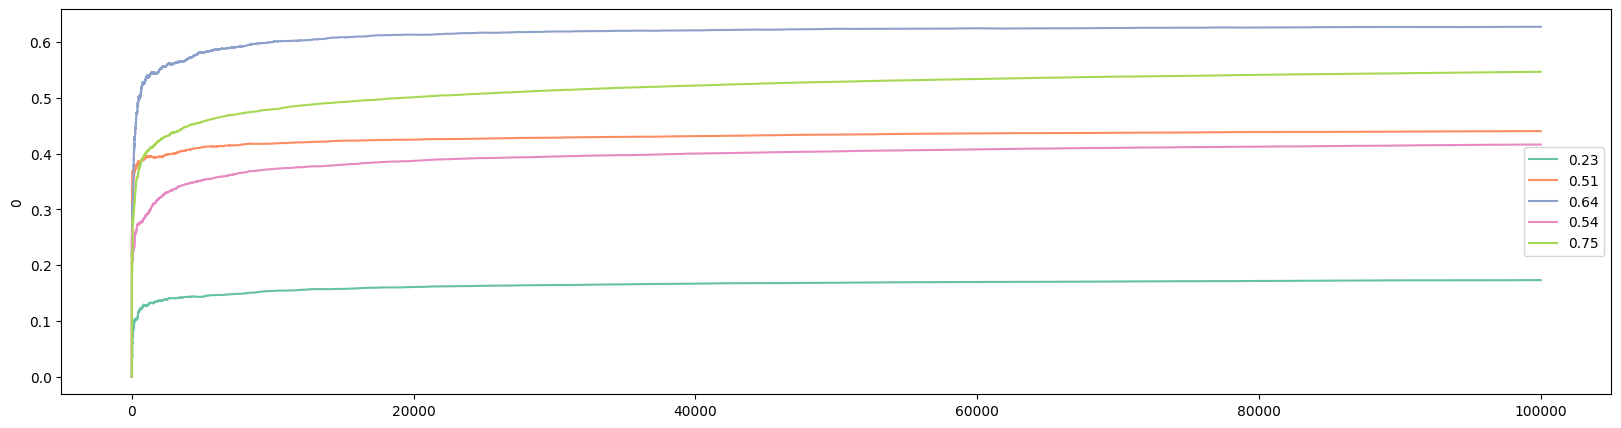
\includegraphics{images/eg.png}
\caption{Epsilon Greedy}
\end{figure}

We can also get the visualization for the first 100 visitors, which shows that the third bandit, the a 0.67 win rate, jumped ahead early:

\begin{Shaded}
\begin{Highlighting}[]
\NormalTok{plot\_history(history}\OperatorTok{=}\NormalTok{eg.history, prob\_true}\OperatorTok{=}\NormalTok{eg.prob\_true, k}\OperatorTok{=}\DecValTok{100}\NormalTok{)}
\end{Highlighting}
\end{Shaded}

\begin{figure}
\centering
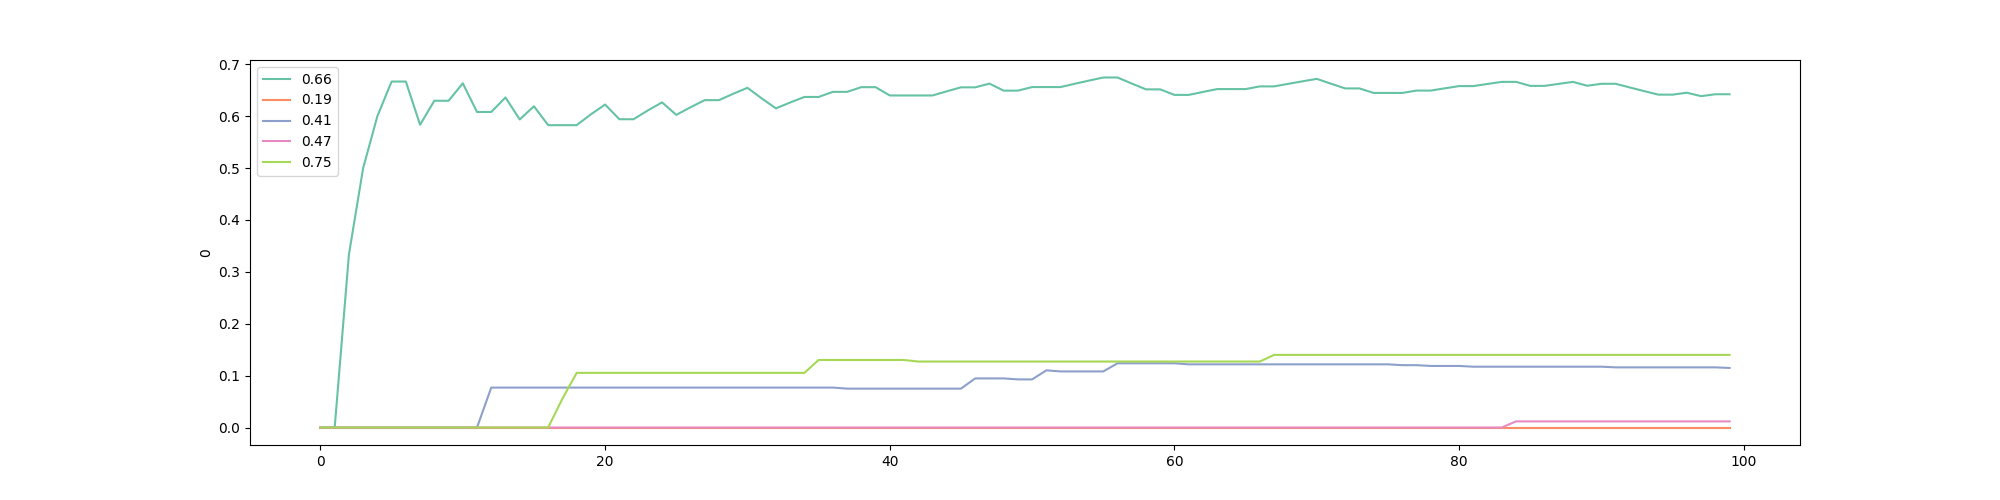
\includegraphics{images/eg_100.png}
\caption{Epsilon Greedy (first 100)}
\end{figure}

\hypertarget{optimistic-initial-values}{%
\section{Optimistic Initial Values}\label{optimistic-initial-values}}

The \texttt{Optimistic\ Initial\ Values} algorithm is one of my favorites (the other being the \texttt{Gradient\ Bandit} algorithm) amongst the algorithms discussed in this article. While \texttt{Epsilon\ Greedy} focused on ``exploit'' and can end up choosing the second-best version, the \texttt{Optimistic\ Initial\ Values} algorithm puts more focus on ``explore'' initially, while staying \texttt{greedy}, i.e., pick the strategy that shows the highest expected win rate. The name of this algorithm informs you about what it does: at the start of the experiment, each bandit is set to have a high expected win rate, i.e., we are ``optimistic'' about each bandit. This ensures that each of them is played a fair number of times initially. If we compare \texttt{Epsilon\ Greedy} to English auctions where the values go up over time, \texttt{Optimistic\ Initial\ Value} is comparable to Dutch auctions where the values go \emph{down} over time. Here is the pseudocode:

\begin{verbatim}
p_init = 5 # a large value as initial win rate for ALL bandits

loop:
    j = argmax(expected bandit win rates)
    x = reward (1 or 0) from playing bandit j
    bandit[j].update_mane(x)
\end{verbatim}

Assuming you already have the code from the \texttt{Epsilon\ Greedy} section, you can add the following method inside the \texttt{BayesianAB} class to run the \texttt{Optimistic\ Initial\ Values} algorithm:

\begin{Shaded}
\begin{Highlighting}[]
    \CommentTok{\#\#\#\#\#\#\#\#\#\#\#\#\#\#\#\#\#\#\#\#}
    \CommentTok{\# optimistic initial values}
    \KeywordTok{def}\NormalTok{ optim\_init\_val(}
            \VariableTok{self}\NormalTok{,}
\NormalTok{            init\_val: }\BuiltInTok{float} \OperatorTok{=} \FloatTok{0.99}\NormalTok{,}
\NormalTok{    ):}

        \VariableTok{self}\NormalTok{.prob\_win }\OperatorTok{=}\NormalTok{ [init\_val] }\OperatorTok{*} \BuiltInTok{len}\NormalTok{(}\VariableTok{self}\NormalTok{.prob\_win)}
        \VariableTok{self}\NormalTok{.history.append(}\VariableTok{self}\NormalTok{.prob\_win.copy())}

        \ControlFlowTok{for}\NormalTok{ k }\KeywordTok{in} \BuiltInTok{range}\NormalTok{(}\DecValTok{1}\NormalTok{, }\VariableTok{self}\NormalTok{.N):}
\NormalTok{            i }\OperatorTok{=}\NormalTok{ np.argmax(}\VariableTok{self}\NormalTok{.prob\_win)}

            \VariableTok{self}\NormalTok{.update(i, k)}

        \ControlFlowTok{return} \VariableTok{self}\NormalTok{.history}
\end{Highlighting}
\end{Shaded}

The only thing new here is the line that assigns \texttt{init\_val} to \texttt{prob\_win} in the beginning. We can execute the following to get results and visualization:

\begin{Shaded}
\begin{Highlighting}[]
\NormalTok{oiv }\OperatorTok{=}\NormalTok{ BayesianAB(N\_bandits)}
\BuiltInTok{print}\NormalTok{(}\SpecialStringTok{f\textquotesingle{}The true win rates: }\SpecialCharTok{\{}\NormalTok{oiv}\SpecialCharTok{.}\NormalTok{prob\_true}\SpecialCharTok{\}}\SpecialStringTok{\textquotesingle{}}\NormalTok{)}
\NormalTok{oiv\_history }\OperatorTok{=}\NormalTok{ oiv.optim\_init\_val(init\_val}\OperatorTok{=}\FloatTok{0.99}\NormalTok{)}
\BuiltInTok{print}\NormalTok{(}\SpecialStringTok{f\textquotesingle{}The observed win rates: }\SpecialCharTok{\{}\NormalTok{oiv}\SpecialCharTok{.}\NormalTok{prob\_win}\SpecialCharTok{\}}\SpecialStringTok{\textquotesingle{}}\NormalTok{)}
\BuiltInTok{print}\NormalTok{(}\SpecialStringTok{f\textquotesingle{}Number of times each bandit was played: }\SpecialCharTok{\{}\NormalTok{oiv}\SpecialCharTok{.}\NormalTok{count}\SpecialCharTok{\}}\SpecialStringTok{\textquotesingle{}}\NormalTok{)}

\CommentTok{\# plot the entire experiment history}
\NormalTok{plot\_history(history}\OperatorTok{=}\NormalTok{oiv.history, prob\_true}\OperatorTok{=}\NormalTok{oiv.prob\_true)}
\end{Highlighting}
\end{Shaded}

And following are outcomes from a typical run:

\begin{verbatim}
The true win rates: [0.6, 0.54, 0.62, 0.14, 0.75]
The observed win rates: [0.6633, 0.7493, 0.7491, 0.7493, 0.7521]
Number of times each bandit was played: [2, 168, 285, 65, 99479]
\end{verbatim}

\begin{figure}
\centering
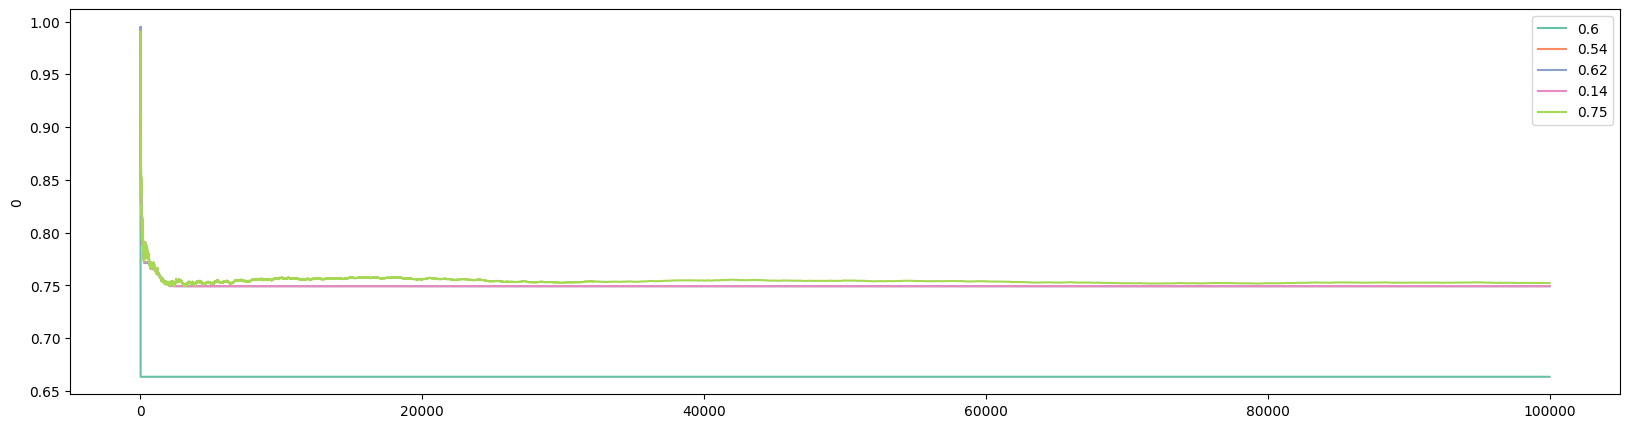
\includegraphics{images/oiv.png}
\caption{Optimistic Initial Values}
\end{figure}

From the visualization below, you can see that the best bandit jumped ahead after about merely 15 visitors:

\begin{figure}
\centering
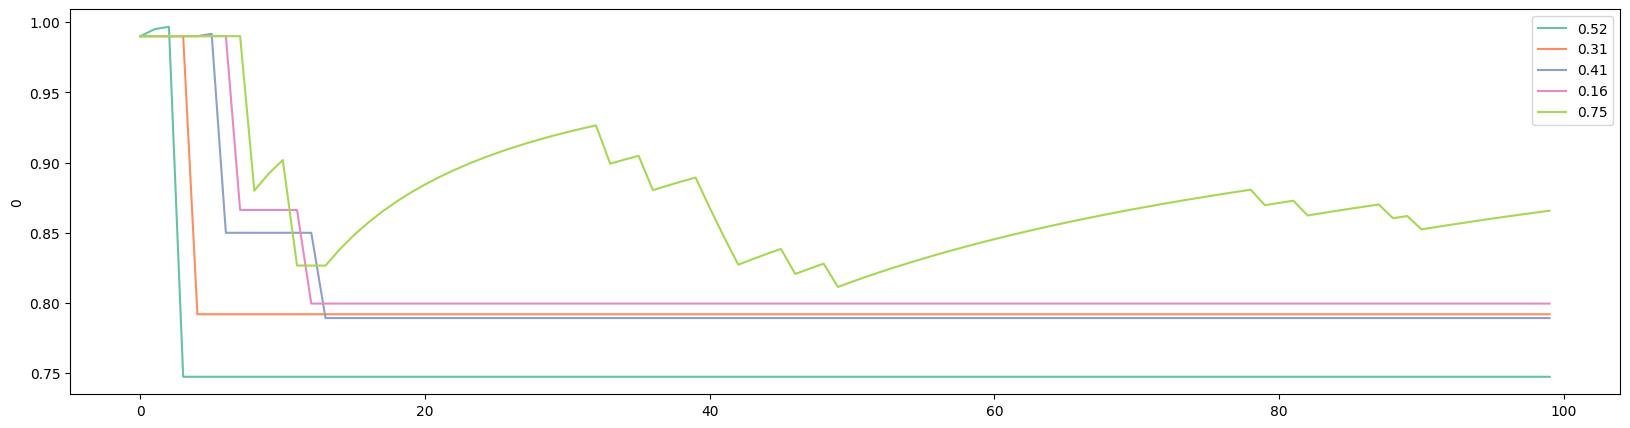
\includegraphics{images/oiv_100.png}
\caption{Optimistic Initial Values (first 100)}
\end{figure}

Note that I set \texttt{init\_val} to 0.99 since we are comparing win rates that can not exceed 1. The larger the initial value, the more the algorithm explores initially. Because the \texttt{Optimistic\ Initial\ Values} algorithm was specifically designed to explore in the beginning, it can ``fall behind'' in reaching the best version, if ever, compared to other algorithms such as \texttt{Epsilon\ Greedy}. Note that if the best bandit is discovered early, the expected win rates of other bandits never converge to their true win rates in \texttt{Optimistic\ Initial\ Values} (but would in \texttt{Epsilon\ Greedy}). This is a common feature of several of the algorithms discussed in this article.

\hypertarget{upper-confidence-bound-ucb}{%
\section{Upper Confidence Bound (UCB)}\label{upper-confidence-bound-ucb}}

The theory of \texttt{UCB} is harder to fully grasp although its intuition and implementation are straightforward. To start, let's look back to the last two algorithms that we have discussed: \texttt{Epsilon\ Greedy} and \texttt{Optimistic\ Initial\ Values}. A common step in the implementation of both of these algorithms is to find the bandit that gives the best \emph{observed} expected win rate. This is why both algorithms are said to be \texttt{greedy}. But can we do better, especially that we know these expected win rates are probabilistic? Put differently, we know that the more a certain bandit was selected, the closer its expected win rate is to its true win rate. But what about those bandits that were rarely picked?

That is where \texttt{Upper\ Confidence\ Bound} comes into play. The idea is that we should not be relying on the observed expected win rates alone in making decisions. We should give each version some ``bonus points'': if a version has been picked a lot, it gets a small bonus; but if a version has barely been barely chosen, it should get a larger bonus because, probabilistically, the observed expected win rate \emph{can} be far from the true win rate if a version has not been played much.

If you are interested in the math, you can read the paper ``\href{https://homes.di.unimi.it/~cesabian/Pubblicazioni/ml-02.pdf}{Finite-time Analysis of the Multiarmed Bandit Problem}''. In the paper, the authors have outlined a function for the ``bonus'', which is commonly known as \texttt{UCB1}:

\[b_j=\sqrt{\frac{2\log{N}}{n_j}}\]

where \(N\) is the total number of visitors at the time of computing the bonus, and \(n_j\) is the number of times that bandit \(j\) was chosen at the time of computing the bonus. Adding \(b\) to the expected win rate gives the \textbf{upper confidence bound}:

\[\text{UCB1}_j=\bar{x}_{n_j}+b_j\]

Here is the pseudocode for \texttt{UCB1}:

\begin{verbatim}
loop:
    Update UCB1 values
    j = argmax(UCB1 values)
    x = reward (1 or 0) from playing bandit j
    bandit[j].update_mean(x)
\end{verbatim}

Adding the following method into \texttt{BayesianAB} will implement \texttt{UCB1}:

\begin{Shaded}
\begin{Highlighting}[]
    \CommentTok{\#\#\#\#\#\#\#\#\#\#\#\#\#\#\#\#\#\#\#\#}
    \CommentTok{\# upper confidence bound (UCB1)}
    \KeywordTok{def}\NormalTok{ ucb1(}
            \VariableTok{self}\NormalTok{,}
\NormalTok{            c}\OperatorTok{=}\DecValTok{1}\NormalTok{,}
\NormalTok{    ):}

        \VariableTok{self}\NormalTok{.history.append(}\VariableTok{self}\NormalTok{.prob\_win.copy())}
\NormalTok{        bandit\_count }\OperatorTok{=}\NormalTok{ [}\FloatTok{0.0001}\NormalTok{] }\OperatorTok{*} \BuiltInTok{len}\NormalTok{(}\VariableTok{self}\NormalTok{.prob\_win)}

        \ControlFlowTok{for}\NormalTok{ k }\KeywordTok{in} \BuiltInTok{range}\NormalTok{(}\DecValTok{1}\NormalTok{, }\VariableTok{self}\NormalTok{.N):}
\NormalTok{            bound }\OperatorTok{=} \VariableTok{self}\NormalTok{.prob\_win }\OperatorTok{+}\NormalTok{ c }\OperatorTok{*}\NormalTok{ np.sqrt(np.divide(}\DecValTok{2} \OperatorTok{*}\NormalTok{ np.log(k), bandit\_count))}
\NormalTok{            i }\OperatorTok{=}\NormalTok{ np.argmax(bound)}

            \VariableTok{self}\NormalTok{.update(i, k)}

            \ControlFlowTok{if}\NormalTok{ bandit\_count[i] }\OperatorTok{\textless{}} \DecValTok{1}\NormalTok{:}
\NormalTok{                bandit\_count[i] }\OperatorTok{=} \DecValTok{0}
\NormalTok{            bandit\_count[i] }\OperatorTok{+=} \DecValTok{1}

        \ControlFlowTok{return} \VariableTok{self}\NormalTok{.history}
\end{Highlighting}
\end{Shaded}

This is very similar to what we had before. One thing to note is that I give a very small initial value (\(0.0001\)) to \texttt{bandit\_count} to avoid the division of zero in the beginning of the experiment. Later, I reversed the value to 0 with the \texttt{if} statement. An alternative approach is to run the first several iterations on all versions before implementing \texttt{UCB1} thereafter.

\texttt{UCB1} has a parameter, \(c\), which controls the degree of exploration. Other things being equal, A larger value \(c\) means a higher reward. The default value is set to 1 in the above script.

Executing the following will give us results and visualization for \texttt{UCB1}:

\begin{Shaded}
\begin{Highlighting}[]
\NormalTok{ucb }\OperatorTok{=}\NormalTok{ BayesianAB(N\_bandits)}
\BuiltInTok{print}\NormalTok{(}\SpecialStringTok{f\textquotesingle{}The true win rates: }\SpecialCharTok{\{}\NormalTok{ucb}\SpecialCharTok{.}\NormalTok{prob\_true}\SpecialCharTok{\}}\SpecialStringTok{\textquotesingle{}}\NormalTok{)}
\NormalTok{ucb\_history }\OperatorTok{=}\NormalTok{ ucb.ucb1()}
\BuiltInTok{print}\NormalTok{(}\SpecialStringTok{f\textquotesingle{}The observed win rates: }\SpecialCharTok{\{}\NormalTok{ucb}\SpecialCharTok{.}\NormalTok{prob\_win}\SpecialCharTok{\}}\SpecialStringTok{\textquotesingle{}}\NormalTok{)}
\BuiltInTok{print}\NormalTok{(}\SpecialStringTok{f\textquotesingle{}Number of times each bandit was played: }\SpecialCharTok{\{}\NormalTok{ucb}\SpecialCharTok{.}\NormalTok{count}\SpecialCharTok{\}}\SpecialStringTok{\textquotesingle{}}\NormalTok{)}

\CommentTok{\# plot the entire experiment history}
\NormalTok{plot\_history(history}\OperatorTok{=}\NormalTok{ucb.history, prob\_true}\OperatorTok{=}\NormalTok{ucb.prob\_true)}
\end{Highlighting}
\end{Shaded}

A typical run gives the following:

\begin{verbatim}
The true win rates: [0.65, 0.12, 0.63, 0.33, 0.75]
The observed win rates: [0.6505, 0.1165, 0.1928, 0.0774, 0.3794]
Number of times each bandit was played: [99470, 77, 103, 67, 282]
\end{verbatim}

\begin{figure}
\centering
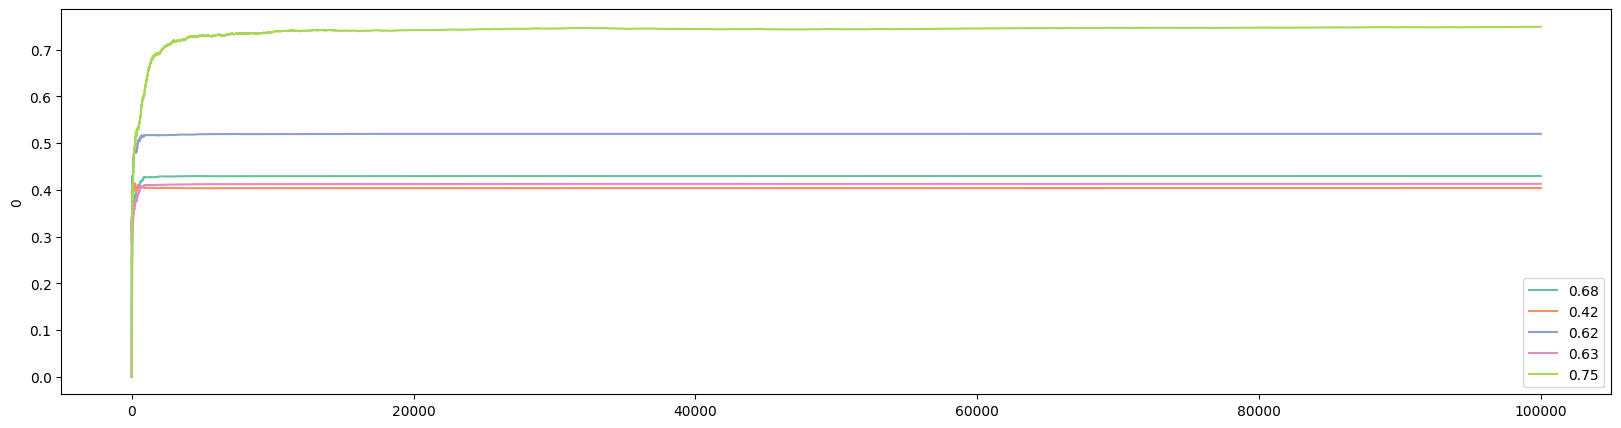
\includegraphics{images/ucb1.png}
\caption{UCB1}
\end{figure}

This particular run shows that \texttt{UCB1} has also failed to identify the best version. Examining the first 100 visitors shows that the bandit with a .65 win rate jumped out early and never looked back. And I do not believe the algorithm can guarantee convergence even with infinite number of visitors:

\begin{figure}
\centering
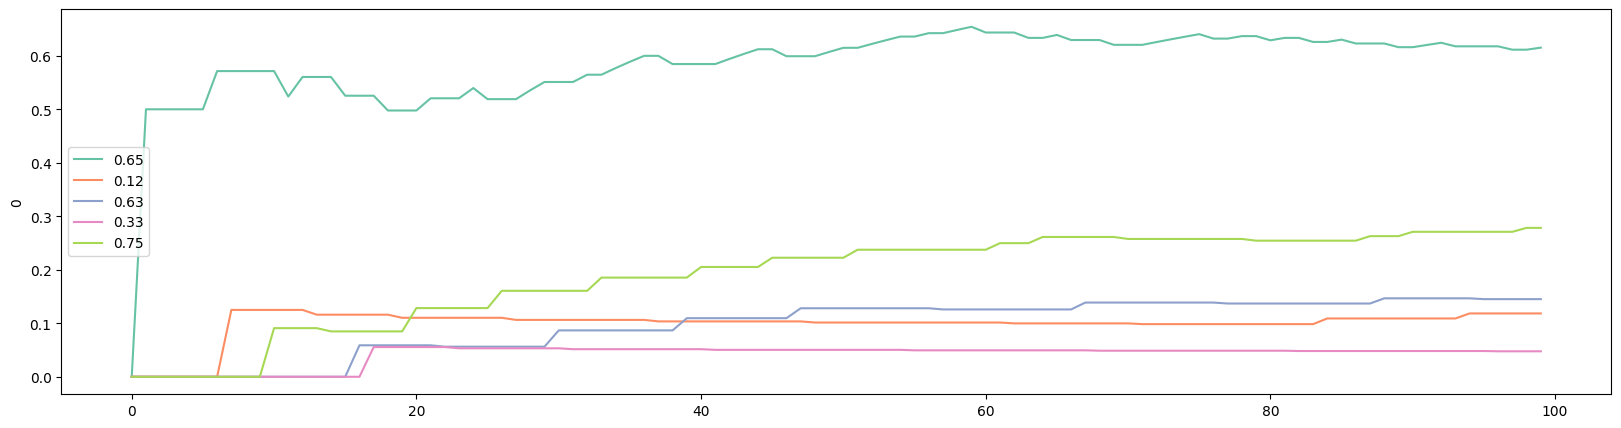
\includegraphics{images/ucb1_100.png}
\caption{UCB1 (first 100)}
\end{figure}

\hypertarget{gradient-bandit-algorithm}{%
\section{Gradient Bandit Algorithm}\label{gradient-bandit-algorithm}}

Another algorithm that does not rely \emph{entirely} on expected win rates is the \texttt{Gradient\ Bandit} algorithm. Not surprisingly, this algorithm is related to gradient ascent. With this algorithm, each bandit's probability of being chosen is determined according to a soft-max distribution:

\[\pi_n(i)=\frac{e^{H_n(i)}}{\sum_{j=1}^{J}{e^{H_n(j)}}}\]

where \(\pi_n(i)\) is the probability of bandit \(i\) being picked for customer \(n\), \(H_n(i)\) is the \emph{preference} for bandit \(i\) at the time customer \(n\) arrives, and \(J\) is the total number of bandits in the experiment. In the case of only two bandits, this specification is the same as the logistic or sigmoid function.

When the first customer arrives, i.e., \(n=1\), it is custom to set the \emph{preference}, \(H_1(j)\), for all \(j\), to 0 so that every bandit has the same probability of getting picked. Suppose bandit \(i\) is picked for customer \(n(\geq1)\), then the \emph{preference} for \(i\) is updated according to:

\[H_{n+1}(i)=H_n(i)+\alpha(x_n - \bar{x}_{n-1})(1-\pi_n(i))\]

whereas the \emph{preferences} for all \(j\neq i\) are updated according to:

\[H_{n+1}(j)=H_n(j)-\alpha(x_n - \bar{x}_{n-1})\pi_n(j)\]

where \(\alpha>0\) is a ``step-size'' parameter.

The intuition of the \texttt{Gradient\ Bandit} algorithm is as follows. When the reward received from picking \(i\) for customer \(n\) is higher than the expected reward, the probability of picking \(i\) in the future (next round) is increased. In our simple case with only two outcomes (buy and not buy), the reward is higher than the expected reward only if customer \(n\) buys.

Let's take a look at the pseudocode:

\begin{verbatim}
H = [0] * number_of_bandits

loop:
  pi = pi(H) # Calculates the soft-max distribution
  i = random.choices(bandits, weights=pi)
  gb.update()
\end{verbatim}

where \texttt{H.update()} updates the values of \(H(i)\) (the bandit that was chosen) and \(H(j)\) (bandits that were not chosen).

Here is the \texttt{Python} implementation for \texttt{Gradient\ Bandit}:

\begin{Shaded}
\begin{Highlighting}[]
    \CommentTok{\#\#\#\#\#\#\#\#\#\#\#\#\#\#\#\#\#\#\#\#}
    \CommentTok{\# gradient\_bandit update}
    \KeywordTok{def}\NormalTok{ gb\_update(}
            \VariableTok{self}\NormalTok{,}
\NormalTok{            i,}
\NormalTok{            k,}
\NormalTok{            a,}
\NormalTok{    ):}

\NormalTok{        outcome }\OperatorTok{=} \VariableTok{self}\NormalTok{.pull(i)}
        \ControlFlowTok{for}\NormalTok{ z }\KeywordTok{in} \BuiltInTok{range}\NormalTok{(}\BuiltInTok{len}\NormalTok{(}\VariableTok{self}\NormalTok{.pref)):}
            \ControlFlowTok{if}\NormalTok{ z }\OperatorTok{==}\NormalTok{ i:}
                \VariableTok{self}\NormalTok{.pref[z] }\OperatorTok{=} \VariableTok{self}\NormalTok{.pref[z] }\OperatorTok{+}\NormalTok{ a }\OperatorTok{*}\NormalTok{ (outcome }\OperatorTok{{-}} \VariableTok{self}\NormalTok{.prob\_win[z]) }\OperatorTok{*}\NormalTok{ (}\DecValTok{1} \OperatorTok{{-}} \VariableTok{self}\NormalTok{.pi[z])}
            \ControlFlowTok{else}\NormalTok{:}
                \VariableTok{self}\NormalTok{.pref[z] }\OperatorTok{=} \VariableTok{self}\NormalTok{.pref[z] }\OperatorTok{{-}}\NormalTok{ a }\OperatorTok{*}\NormalTok{ (outcome }\OperatorTok{{-}} \VariableTok{self}\NormalTok{.prob\_win[z]) }\OperatorTok{*} \VariableTok{self}\NormalTok{.pi[z]}

        \VariableTok{self}\NormalTok{.prob\_win[i] }\OperatorTok{=}\NormalTok{ (}\VariableTok{self}\NormalTok{.prob\_win[i] }\OperatorTok{*}\NormalTok{ k }\OperatorTok{+}\NormalTok{ outcome) }\OperatorTok{/}\NormalTok{ (k }\OperatorTok{+} \DecValTok{1}\NormalTok{)}

        \ControlFlowTok{return} \VariableTok{self}\NormalTok{.pref}

    \CommentTok{\# gradient bandit algorithm}
    \KeywordTok{def}\NormalTok{ gradient\_bandit(}
            \VariableTok{self}\NormalTok{,}
\NormalTok{            a}\OperatorTok{=}\FloatTok{0.2}\NormalTok{,}
\NormalTok{    ):}

        \VariableTok{self}\NormalTok{.history.append([}\VariableTok{self}\NormalTok{.pi.copy(),}
                             \VariableTok{self}\NormalTok{.pref.copy(),}
                             \VariableTok{self}\NormalTok{.prob\_win.copy()])}

        \ControlFlowTok{for}\NormalTok{ k }\KeywordTok{in} \BuiltInTok{range}\NormalTok{(}\DecValTok{1}\NormalTok{, }\VariableTok{self}\NormalTok{.N):}
            \VariableTok{self}\NormalTok{.pi }\OperatorTok{=}\NormalTok{ np.exp(}\VariableTok{self}\NormalTok{.pref) }\OperatorTok{/} \BuiltInTok{sum}\NormalTok{(np.exp(}\VariableTok{self}\NormalTok{.pref))}
\NormalTok{            pick }\OperatorTok{=}\NormalTok{ random.choices(np.arange(}\BuiltInTok{len}\NormalTok{(}\VariableTok{self}\NormalTok{.pref)), weights}\OperatorTok{=}\VariableTok{self}\NormalTok{.pi)}
\NormalTok{            i }\OperatorTok{=}\NormalTok{ pick[}\DecValTok{0}\NormalTok{]}
            \VariableTok{self}\NormalTok{.pref }\OperatorTok{=} \VariableTok{self}\NormalTok{.gb\_update(i, k, a)}

            \VariableTok{self}\NormalTok{.count[i] }\OperatorTok{+=} \DecValTok{1}
            \VariableTok{self}\NormalTok{.history.append([}\VariableTok{self}\NormalTok{.pi.copy(),}
                                 \VariableTok{self}\NormalTok{.pref.copy(),}
                                 \VariableTok{self}\NormalTok{.prob\_win.copy()])}
            \VariableTok{self}\NormalTok{.history\_bandit.append(i)  }\CommentTok{\# for Monte Carlo}

        \ControlFlowTok{return} \VariableTok{self}\NormalTok{.history}
\end{Highlighting}
\end{Shaded}

Here are some notes on the \texttt{Python} implementation of the \texttt{Gradient\ Bandit} algorithm:
1. We have already initiated \texttt{pref} and \texttt{pi} at the start of the \texttt{BayesianAB} class;
2. As discussed in the pseudocode, a new function, \texttt{gb\_update()}, is necessary since we need to update the preference function for every bandit in each round;
3. The \texttt{gradient\_bandit()} function takes 1 parameter: \(a\), which is the step-size parameter. The default value of \(a\) is set to 0.2. The smaller the value of \(a\), the more the algorithm explores;
4. \texttt{gradient\_bandit()} saves \texttt{history} differently: each row in \texttt{history} is an array of 3 lists. In order to examine the performance of the \texttt{Gradient\ Bandit} algorithm, we not only save the expected win rates, but also preferences and the values from the soft-max distribution, \(\pi(i)\);
5. The function \texttt{choices()} from the \texttt{random} library picks a value from a list based on \texttt{weights}. In this case, the weights is given by the soft-max distribution;

Because \texttt{gradient\_bandit()} saves arrays in \texttt{history}, we also need to update the \texttt{plot\_history()} function:

\begin{Shaded}
\begin{Highlighting}[]
\KeywordTok{def}\NormalTok{ plot\_history(}
\NormalTok{        history: }\BuiltInTok{list}\NormalTok{,}
\NormalTok{        prob\_true: }\BuiltInTok{list}\NormalTok{,}
\NormalTok{        col}\OperatorTok{=}\DecValTok{2}\NormalTok{,}
\NormalTok{        k}\OperatorTok{=}\NormalTok{N,}
\NormalTok{):}
    \ControlFlowTok{if} \BuiltInTok{type}\NormalTok{(history[}\DecValTok{0}\NormalTok{][}\DecValTok{0}\NormalTok{]) }\OperatorTok{==} \BuiltInTok{list}\NormalTok{:  }\CommentTok{\# To accommodate gradient bandit}
\NormalTok{        df\_history }\OperatorTok{=}\NormalTok{ pd.DataFrame([arr[col] }\ControlFlowTok{for}\NormalTok{ arr }\KeywordTok{in}\NormalTok{ history][:k])}
    \ControlFlowTok{else}\NormalTok{:}
\NormalTok{        df\_history }\OperatorTok{=}\NormalTok{ pd.DataFrame(history[:k])}

\NormalTok{    plt.figure(figsize}\OperatorTok{=}\NormalTok{(}\DecValTok{20}\NormalTok{, }\DecValTok{5}\NormalTok{))}

    \CommentTok{\# Define the color palette}
\NormalTok{    colors }\OperatorTok{=}\NormalTok{ sns.color\_palette(}\StringTok{"Set2"}\NormalTok{, }\BuiltInTok{len}\NormalTok{(prob\_true))}

    \ControlFlowTok{for}\NormalTok{ i }\KeywordTok{in} \BuiltInTok{range}\NormalTok{(}\BuiltInTok{len}\NormalTok{(prob\_true)):}
\NormalTok{        sns.lineplot(x}\OperatorTok{=}\NormalTok{df\_history.index, y}\OperatorTok{=}\NormalTok{df\_history[i], color}\OperatorTok{=}\NormalTok{colors[i])}

    \CommentTok{\# Create custom legend using prob\_true and colors}
\NormalTok{    custom\_legend }\OperatorTok{=}\NormalTok{ [plt.Line2D([], [], color}\OperatorTok{=}\NormalTok{colors[i], label}\OperatorTok{=}\NormalTok{prob\_true[i]) }\ControlFlowTok{for}\NormalTok{ i }\KeywordTok{in} \BuiltInTok{range}\NormalTok{(}\BuiltInTok{len}\NormalTok{(prob\_true))]}
\NormalTok{    plt.legend(handles}\OperatorTok{=}\NormalTok{custom\_legend)}
\end{Highlighting}
\end{Shaded}

The updates occurred in

\begin{Shaded}
\begin{Highlighting}[]
    \ControlFlowTok{if} \BuiltInTok{type}\NormalTok{(history[}\DecValTok{0}\NormalTok{][}\DecValTok{0}\NormalTok{]) }\OperatorTok{==} \BuiltInTok{list}\NormalTok{:  }\CommentTok{\# To accommodate gradient bandit}
\NormalTok{        df\_history }\OperatorTok{=}\NormalTok{ pd.DataFrame([arr[col] }\ControlFlowTok{for}\NormalTok{ arr }\KeywordTok{in}\NormalTok{ history][:k])}
    \ControlFlowTok{else}\NormalTok{:}
\NormalTok{        df\_history }\OperatorTok{=}\NormalTok{ pd.DataFrame(history[:k])}
\end{Highlighting}
\end{Shaded}

with the added parameter \texttt{col}. This is to accommodate the arrays saved in history by \texttt{gradient\_bandit()}. The \texttt{if} statement checks whether the first element in \texttt{history} is a \texttt{list}. If it is, then \texttt{history} was saved from \texttt{gradient\_bandit()} and we would need to extract the specific column, given by \texttt{col}, for plotting. The default value of \texttt{col} is 2, which is to plot the history of the win rates.

Executing the following will run the \texttt{Gradient\ Bandit} algorithm:

\begin{Shaded}
\begin{Highlighting}[]
\CommentTok{\# Gradient bandit}
\NormalTok{gb }\OperatorTok{=}\NormalTok{ BayesianAB(N\_bandits)}
\BuiltInTok{print}\NormalTok{(}\SpecialStringTok{f\textquotesingle{}The true win rates: }\SpecialCharTok{\{}\NormalTok{gb}\SpecialCharTok{.}\NormalTok{prob\_true}\SpecialCharTok{\}}\SpecialStringTok{\textquotesingle{}}\NormalTok{)}
\NormalTok{gb\_history }\OperatorTok{=}\NormalTok{ gb.gradient\_bandit()}
\BuiltInTok{print}\NormalTok{(}\SpecialStringTok{f\textquotesingle{}The observed win rates: }\SpecialCharTok{\{}\NormalTok{gb}\SpecialCharTok{.}\NormalTok{prob\_win}\SpecialCharTok{\}}\SpecialStringTok{\textquotesingle{}}\NormalTok{)}
\BuiltInTok{print}\NormalTok{(}\SpecialStringTok{f\textquotesingle{}Number of times each bandit was played: }\SpecialCharTok{\{}\NormalTok{gb}\SpecialCharTok{.}\NormalTok{count}\SpecialCharTok{\}}\SpecialStringTok{\textquotesingle{}}\NormalTok{)}

\CommentTok{\# plot the entire experiment history}
\NormalTok{plot\_history(history}\OperatorTok{=}\NormalTok{gb.history, prob\_true}\OperatorTok{=}\NormalTok{gb.prob\_true)}
\end{Highlighting}
\end{Shaded}

Here are results from a typical run:

\begin{verbatim}
The true win rates: [0.17, 0.56, 0.17, 0.7, 0.75]
The observed win rates: [0.2564, 0.5514, 0.0105, 0.6636, 0.7498]
Number of times each bandit was played: [35, 67, 22, 196, 99679]
\end{verbatim}

\begin{figure}
\centering
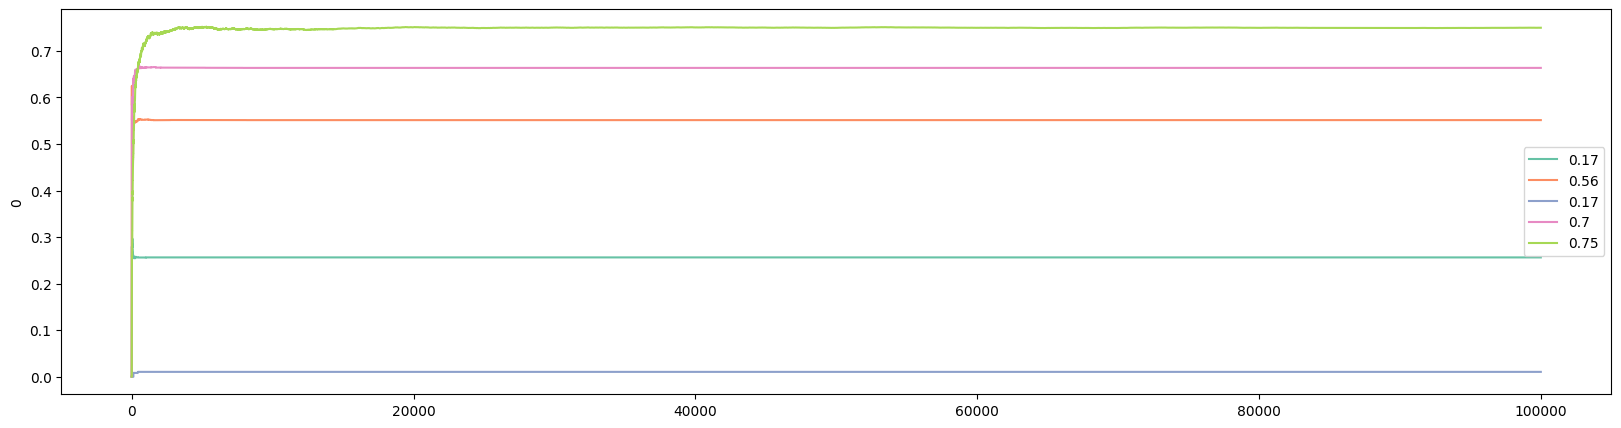
\includegraphics{images/gb.png}
\caption{Gradient Bandit}
\end{figure}

As usual, we can examine what happened after 100 customers. Interestingly, the bandit with the highest win rate did not lead after only 100 customers:

\begin{figure}
\centering
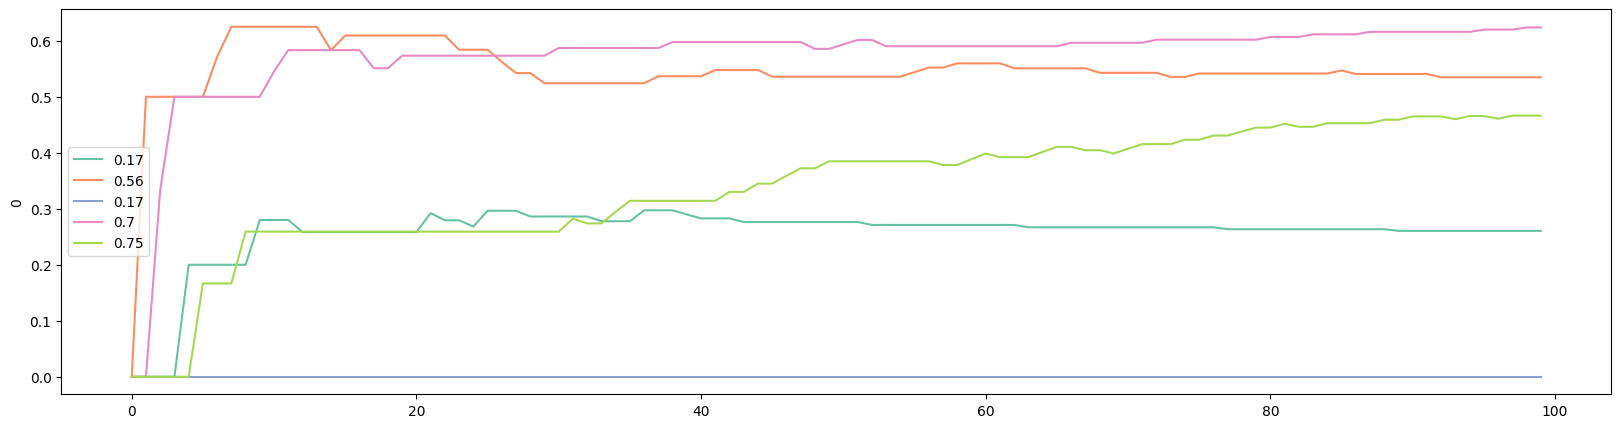
\includegraphics{images/gb_100.png}
\caption{Gradient Bandit (first 100)}
\end{figure}

We can plot the evolution of the \texttt{preference} with the following:

\begin{Shaded}
\begin{Highlighting}[]
\CommentTok{\# plot preference}
\NormalTok{plot\_history(history}\OperatorTok{=}\NormalTok{gb.history, prob\_true}\OperatorTok{=}\NormalTok{gb.prob\_true, col}\OperatorTok{=}\DecValTok{1}\NormalTok{)}
\end{Highlighting}
\end{Shaded}

\begin{figure}
\centering
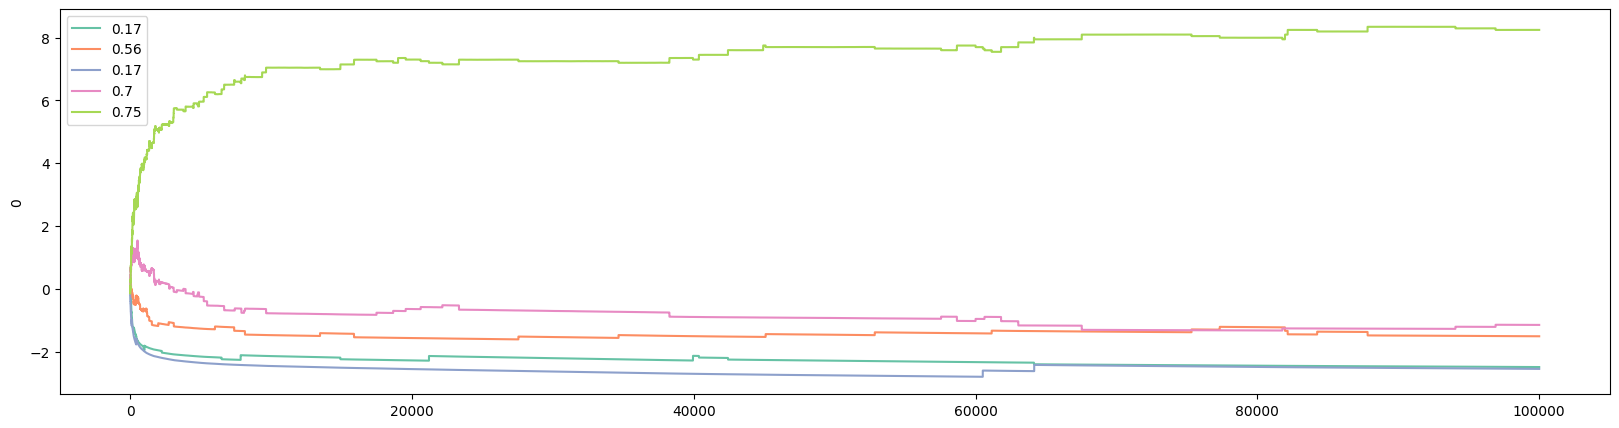
\includegraphics{images/gb_pref.png}
\caption{Gradient Bandit (preference)}
\end{figure}

And plot the soft-max function with the following:

\begin{Shaded}
\begin{Highlighting}[]
\CommentTok{\# plot pi}
\NormalTok{plot\_history(history}\OperatorTok{=}\NormalTok{gb.history, prob\_true}\OperatorTok{=}\NormalTok{gb.prob\_true, col}\OperatorTok{=}\DecValTok{0}\NormalTok{)}
\end{Highlighting}
\end{Shaded}

\begin{figure}
\centering
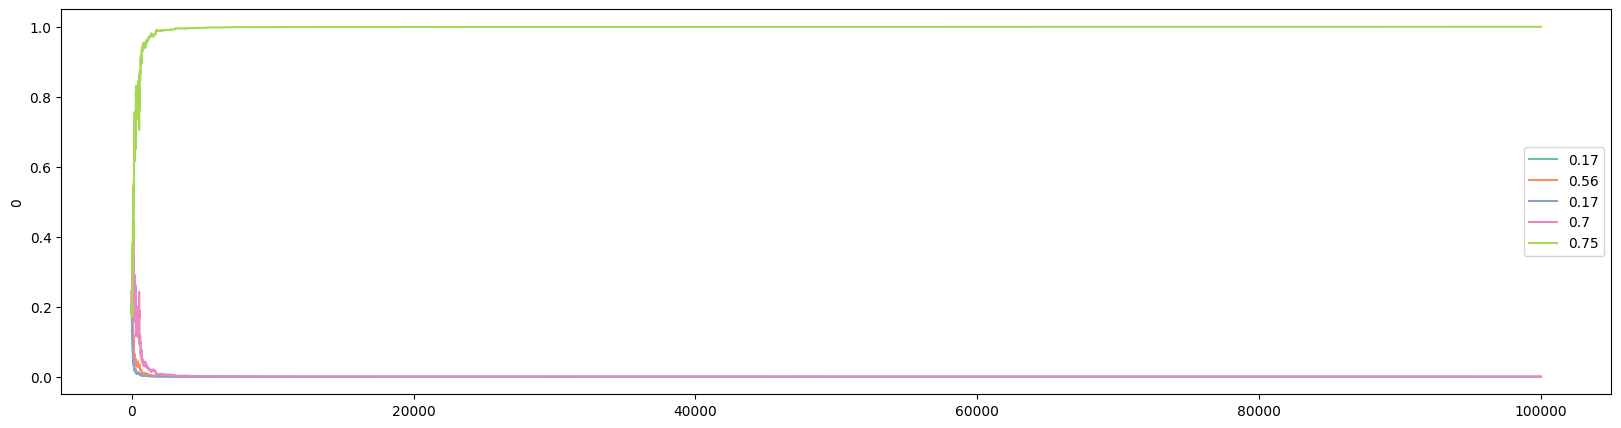
\includegraphics{images/gb_pi.png}
\caption{Gradient Bandit (pi)}
\end{figure}

There are several reasons why the \texttt{Gradient\ Bandit} algorithm is one of my favorites:
1. Economists are familiar with the idea of using \texttt{preference} to model choices;
2. Economists are familiar with \texttt{logistic} function, used in logistic regression, which is the special case of \texttt{soft-max} with only two bandits;
3. One of my research areas is conflict and contest, in which the \texttt{soft-max} function, known as ``contest success function'', is widely used in the literature.

\hypertarget{thompson-sampling-bayesian-bandits}{%
\section{Thompson Sampling (Bayesian Bandits)}\label{thompson-sampling-bayesian-bandits}}

\texttt{Thompson\ Sampling}, or \texttt{Bayesian\ Bandits}, takes another (big) step forward. In our discussion on \texttt{Upper\ Confidence\ Bound}, we acknowledged the fact that using only the expected win rate to represent the performance of a bandit is not accurate. To tackle this, \texttt{UCB1} adds a ``bonus'': the bonus is smaller for the bandits that were played more, and larger for the bandits that were played less. Then in our discussion on \texttt{Gradient\ Bandit}, each bandit's chance of being picked is described by a soft-max distribution.

To push these ideas further, and as the name \texttt{Thompson\ Sampling} has hinted, we ask if we could construct a probability distribution to describe the expected win rates of all the bandits. As it turns out, this is possible, as everything, including parameters, are considered random variables in Bayesian Statistics. For example, with Normal Distribution, we often speak about fixed values of mean and variance. But in Bayesian Statistics, the mean and variance of a Normal Distribution are two random variables and they can be described by probability distributions.

The mathematical derivation of \texttt{Thompson\ Sampling} requires the use of \href{https://en.wikipedia.org/wiki/Conjugate_prior}{conjugate prior}, which I will discuss here briefly, before returning to the \texttt{Python} implementation of \texttt{Thompson\ Sampling}.

\hypertarget{conjugate-prior}{%
\section{Conjugate Prior}\label{conjugate-prior}}

Recall the Bayes Rule:
\[p(\theta \mid X)=\frac{p(X \mid \theta)p(\theta)}{p(X)}\]
where the four parts are called, respectively
* \(p(\theta \mid X)\): Posterior distribution
* \(p(X \mid \theta)\): Likelihood function
* \(p(\theta)\): Prior probability distribution
* \(p(X)\): Evidence

In Bayesian Statistics, if the posterior distribution is in the same probability distribution family as the prior probability distribution, the prior and posterior are then called conjugate distributions, and the prior is called a \textbf{conjugate prior} for the likelihood function.

With conjugate priors, the updating in a Bayesian approach reduces to the updates of hyperparameters that are used to describe both the prior and posterior distributions, since they are the same. I will leave the details to a Statistics textbook, but for our purpose, since our example concerns of binary outcomes (buy or not buy), our likelihood function is that of Bernoulli. As it turns out, the conjugate prior for a Bernoulli likelihood function is the Beta distribution, which has two hyperparameters: \(\alpha\) and \(\beta\).

Now that we have established that Beta distribution is the conjugate prior for Bernoulli, the problem of \texttt{Thompson\ Sampling} is reduced to
1. sample from the Beta distribution
2. find the highest expected value

\hypertarget{thompson-sampling-code}{%
\section{Thompson Sampling: Code}\label{thompson-sampling-code}}

Since \texttt{Thompson\ Sampling} is mechanical different from the previous algorithms, we need to develop special functions and methods to implement \texttt{Thompson\ Sampling}. Here is a pseudocode:

\begin{verbatim}
loop:
    sampling from Beta function for bandit b
    j = argmax(b.sample() for b bandits)
    x = reward (1 or 0) from playing bandit j
    bandit[j].bb_update(x)
\end{verbatim}

The function that needs to be added is \texttt{bb\_update()}. Here is the full \texttt{Python} implementation:

\begin{Shaded}
\begin{Highlighting}[]
\ImportTok{from}\NormalTok{ scipy.stats }\ImportTok{import}\NormalTok{ beta}

    \CommentTok{\#\#\#\#\#\#\#\#\#\#\#\#\#\#\#\#\#\#\#\#}
    \CommentTok{\# bayesian\_bandits update}
    \KeywordTok{def}\NormalTok{ bb\_update(}
            \VariableTok{self}\NormalTok{,}
\NormalTok{            a,}
\NormalTok{            b,}
\NormalTok{            i,}
\NormalTok{    ):}

\NormalTok{        outcome }\OperatorTok{=} \VariableTok{self}\NormalTok{.pull(i)}
\NormalTok{        a[i] }\OperatorTok{+=}\NormalTok{ outcome}
\NormalTok{        b[i] }\OperatorTok{+=} \DecValTok{1} \OperatorTok{{-}}\NormalTok{ outcome}
        \VariableTok{self}\NormalTok{.count[i] }\OperatorTok{+=} \DecValTok{1}

        \ControlFlowTok{return}\NormalTok{ a, b}

    \CommentTok{\# Bayesian bandits}
    \CommentTok{\# For Bernoulli distribution, the conjugate prior is Beta distribution}
    \KeywordTok{def}\NormalTok{ bayesian\_bandits(}
            \VariableTok{self}\NormalTok{,}
\NormalTok{            sample\_size: }\BuiltInTok{int} \OperatorTok{=} \DecValTok{10}\NormalTok{,}
\NormalTok{    ):}

\NormalTok{        a\_hist, b\_hist }\OperatorTok{=}\NormalTok{ [], []}
\NormalTok{        a\_hist.append(}\VariableTok{self}\NormalTok{.alpha.copy())}
\NormalTok{        b\_hist.append(}\VariableTok{self}\NormalTok{.beta.copy())}

        \ControlFlowTok{for}\NormalTok{ k }\KeywordTok{in} \BuiltInTok{range}\NormalTok{(}\DecValTok{1}\NormalTok{, }\VariableTok{self}\NormalTok{.N):}
\NormalTok{            sample\_max }\OperatorTok{=}\NormalTok{ []}

            \ControlFlowTok{for}\NormalTok{ m }\KeywordTok{in} \BuiltInTok{range}\NormalTok{(}\BuiltInTok{len}\NormalTok{(}\VariableTok{self}\NormalTok{.prob\_true)):}
\NormalTok{                m\_max }\OperatorTok{=}\NormalTok{ np.}\BuiltInTok{max}\NormalTok{(np.random.beta(}\VariableTok{self}\NormalTok{.alpha[m], }\VariableTok{self}\NormalTok{.beta[m], sample\_size))}
\NormalTok{                sample\_max.append(m\_max.copy())}

\NormalTok{            i }\OperatorTok{=}\NormalTok{ np.argmax(sample\_max)}

            \VariableTok{self}\NormalTok{.alpha, }\VariableTok{self}\NormalTok{.beta }\OperatorTok{=} \VariableTok{self}\NormalTok{.bb\_update(}\VariableTok{self}\NormalTok{.alpha, }\VariableTok{self}\NormalTok{.beta, i)}
\NormalTok{            a\_hist.append(}\VariableTok{self}\NormalTok{.alpha.copy())}
\NormalTok{            b\_hist.append(}\VariableTok{self}\NormalTok{.beta.copy())}
            \VariableTok{self}\NormalTok{.history\_bandit.append(i)  }\CommentTok{\# for Monte Carlo}

        \VariableTok{self}\NormalTok{.history }\OperatorTok{=}\NormalTok{ [a\_hist, b\_hist]}
        \ControlFlowTok{return} \VariableTok{self}\NormalTok{.history}
\end{Highlighting}
\end{Shaded}

Let's walk through this script:
1. We have already initiated \texttt{alpha} and \texttt{beta} at the start of the \texttt{BayesianAB} class. They are the hyperparameters in the Beta distribution;
2. We import \texttt{beta} from \texttt{scipy.stats} since the conjugate prior for Bernoulli distribution is the Beta distribution.
3. The function \texttt{bb\_update()} updates the hyperparameter values based on the outcome from the last visitor for bandit \(i\): if the outcome was \texttt{True}, then the value of \texttt{alpha} increases by 1; otherwise, the value of \texttt{beta} increases by 1.

For the actual implementation of the \texttt{Bayesian\ Bandits} in the \texttt{bayesian\_bandits()} method, it is largely consistent with what we have been doing in other algorithms. The main differences include:
1. Instead of storing the history of outcomes, we store the history of the values of \texttt{alpha} and \texttt{beta};
2. In each iteration, we first find the maximum value from the sample of values of each bandit, then pick the best from this set of \emph{maximum} values;
3. As described earlier, the updating is different. Instead of updating the mean, we update the values of \texttt{alpha} and \texttt{beta}.

Due to these changes, we also need a new function for visualizing the \texttt{history} returned by \texttt{bayesian\_bandits()}:

\begin{Shaded}
\begin{Highlighting}[]
\KeywordTok{def}\NormalTok{ bb\_plot\_history(}
\NormalTok{        history: }\BuiltInTok{list}\NormalTok{,}
\NormalTok{        prob\_true: }\BuiltInTok{list}\NormalTok{,}
\NormalTok{        k}\OperatorTok{={-}}\DecValTok{1}\NormalTok{,}
\NormalTok{):}
\NormalTok{    x }\OperatorTok{=}\NormalTok{ np.linspace(}\DecValTok{0}\NormalTok{, }\DecValTok{1}\NormalTok{, }\DecValTok{100}\NormalTok{)}
\NormalTok{    legend\_str }\OperatorTok{=}\NormalTok{ [[]] }\OperatorTok{*} \BuiltInTok{len}\NormalTok{(prob\_true)}
\NormalTok{    plt.figure(figsize}\OperatorTok{=}\NormalTok{(}\DecValTok{20}\NormalTok{, }\DecValTok{5}\NormalTok{))}

    \ControlFlowTok{for}\NormalTok{ i }\KeywordTok{in} \BuiltInTok{range}\NormalTok{(}\BuiltInTok{len}\NormalTok{(prob\_true)):}
\NormalTok{        a }\OperatorTok{=}\NormalTok{ history[}\DecValTok{0}\NormalTok{][k][i]}
\NormalTok{        b }\OperatorTok{=}\NormalTok{ history[}\DecValTok{1}\NormalTok{][k][i]}
\NormalTok{        y }\OperatorTok{=}\NormalTok{ beta.pdf(x, a, b)}
\NormalTok{        legend\_str[i] }\OperatorTok{=} \SpecialStringTok{f\textquotesingle{}}\SpecialCharTok{\{}\NormalTok{prob\_true[i]}\SpecialCharTok{\}}\SpecialStringTok{, alpha: }\SpecialCharTok{\{}\NormalTok{a}\SpecialCharTok{\}}\SpecialStringTok{, beta: }\SpecialCharTok{\{}\NormalTok{b}\SpecialCharTok{\}}\SpecialStringTok{\textquotesingle{}}
\NormalTok{        plt.plot(x, y)}

\NormalTok{    plt.legend(legend\_str)}
\end{Highlighting}
\end{Shaded}

We can now run a simulate for \texttt{Thompson\ Sampling} by executing the following:

\begin{Shaded}
\begin{Highlighting}[]
\NormalTok{bb }\OperatorTok{=}\NormalTok{ BayesianAB(N\_bandits)}
\BuiltInTok{print}\NormalTok{(}\SpecialStringTok{f\textquotesingle{}The true win rates: }\SpecialCharTok{\{}\NormalTok{bb}\SpecialCharTok{.}\NormalTok{prob\_true}\SpecialCharTok{\}}\SpecialStringTok{\textquotesingle{}}\NormalTok{)}
\NormalTok{bb\_history }\OperatorTok{=}\NormalTok{ bb.bayesian\_bandits(sample\_size}\OperatorTok{=}\DecValTok{10}\NormalTok{)}
\BuiltInTok{print}\NormalTok{(}\SpecialStringTok{f\textquotesingle{}The observed win rates: }\SpecialCharTok{\{}\NormalTok{np}\SpecialCharTok{.}\NormalTok{divide(bb.history[}\DecValTok{0}\NormalTok{][}\OperatorTok{{-}}\DecValTok{1}\NormalTok{], bb.count)}\SpecialCharTok{\}}\SpecialStringTok{\textquotesingle{}}\NormalTok{)}
\BuiltInTok{print}\NormalTok{(}\SpecialStringTok{f\textquotesingle{}Number of times each bandit was played: }\SpecialCharTok{\{}\NormalTok{bb}\SpecialCharTok{.}\NormalTok{count}\SpecialCharTok{\}}\SpecialStringTok{\textquotesingle{}}\NormalTok{)}

\CommentTok{\# plot the entire experiment history}
\NormalTok{bb\_plot\_history(history}\OperatorTok{=}\NormalTok{bb.history, prob\_true}\OperatorTok{=}\NormalTok{bb.prob\_true)}
\end{Highlighting}
\end{Shaded}

Outcomes from a typical run look like the following:

\begin{verbatim}
The true win rates: [0.15, 0.67, 0.11, 0.47, 0.75]
The observed win rates: [0.1, 0.6563, 0.1667, 0.4545, 0.7500]
Number of times each bandit was played: [10, 355, 12, 44, 99578]
\end{verbatim}

\begin{figure}
\centering
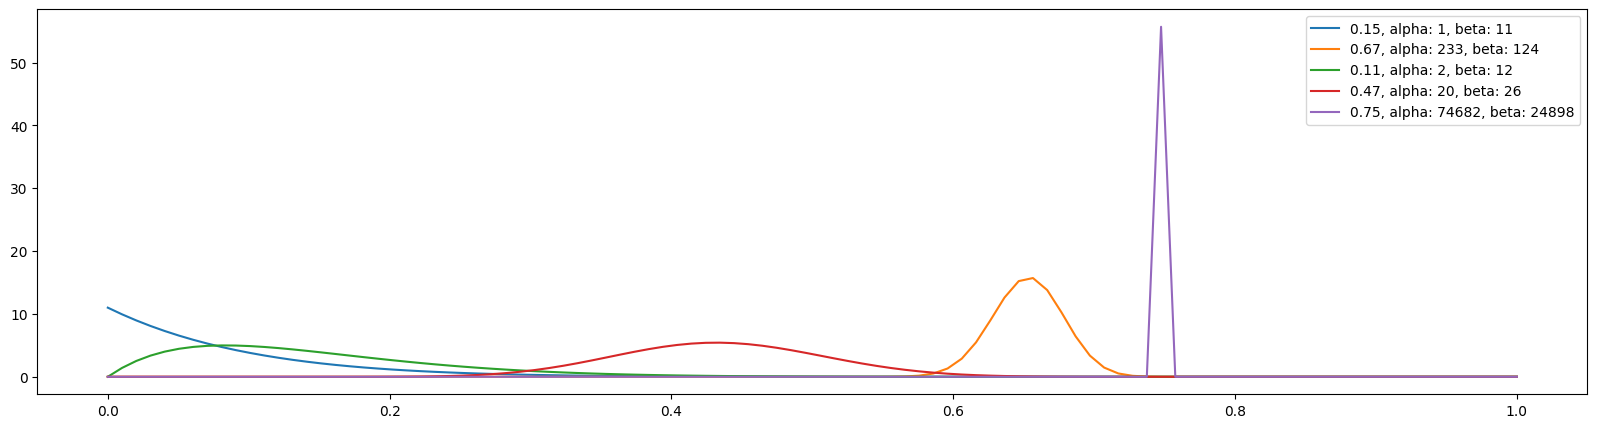
\includegraphics{images/bb.png}
\caption{Bayesian Bandits}
\end{figure}

It is also interesting to look at what happened after only 100 visitors:

\begin{figure}
\centering
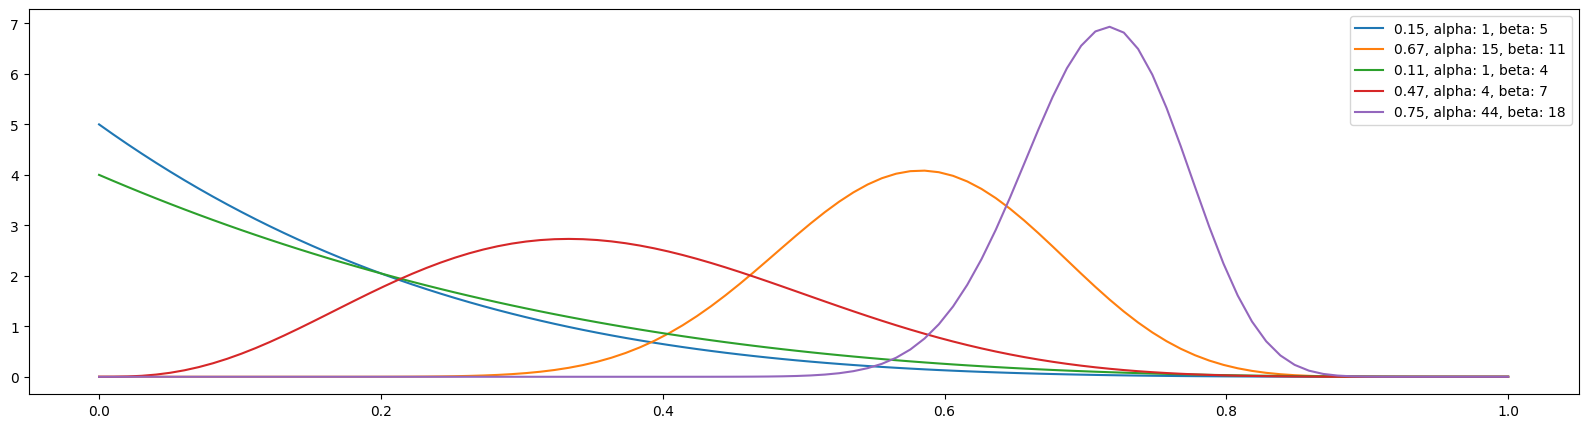
\includegraphics{images/bb_100.png}
\caption{Bayesian Bandits (first 100)}
\end{figure}

Two differences between \texttt{Thompson\ Sampling} and the other algorithms we have discussed should be noted. First, as already mentioned, \texttt{Thompson\ Sampling} attempts to build a distribution for the bandits. Comparing the two visuals from 100 visitors and all visitors shows that, although the best version has jumped out early, the distribution is much tighter/narrower at the end of the experiment, indicating greater ``confidence'' for the estimated expected win rate. Second, and importantly, the \texttt{Thompson\ Sampling} algorithm has no problem distinguishing between a bandit with a 0.67 win rate and the best version with a win rate of 0.75.

\hypertarget{comparing-the-algorithms}{%
\section{Comparing the Algorithms}\label{comparing-the-algorithms}}

It is important to compare the five algorithms in various settings. Following Sutton and Barto (2020), I conduct a 5-armed testbed. The idea of the testbed is to run the algorithms many times, say 2,000, then calculates the success rate, which is the percentage that the best bandit was picked in each round. For example, suppose we run the \texttt{Epsilon\ Greedy} algorithm 2,000 times with different win rates. We look at the bandit picked on the 100th visitor and found that, out of the 2,000 runs the best bandit was picked 800 times. Then at the 100th round/visitor, the success rate was 0.4. When we developed the \texttt{BayesianAB} class, we were already anticipating the implementation of the testbed. Specifically, in the following functions/methods:
* \texttt{update()}
* \texttt{gradient\_bandit()}
* \texttt{bayesian\_bandits()}

there is

\begin{Shaded}
\begin{Highlighting}[]
\VariableTok{self}\NormalTok{.history\_bandit.append(i)}
\end{Highlighting}
\end{Shaded}

which records the which bandit was picked at each round. The parameters \texttt{p\_max}, \texttt{p\_diff}, and \texttt{p\_min} also allow the \texttt{BayesianAB} class to generate different win rates. We will now develop a script to implement the testbed where the \texttt{BayesianAB} class is imported and called:

\begin{Shaded}
\begin{Highlighting}[]
\ImportTok{import}\NormalTok{ numpy }\ImportTok{as}\NormalTok{ np}
\ImportTok{import}\NormalTok{ pandas }\ImportTok{as}\NormalTok{ pd}
\ImportTok{import}\NormalTok{ matplotlib.pyplot }\ImportTok{as}\NormalTok{ plt}
\ImportTok{import}\NormalTok{ seaborn }\ImportTok{as}\NormalTok{ sns}
\ImportTok{from}\NormalTok{ multiprocessing }\ImportTok{import}\NormalTok{ Pool, cpu\_count}
\ImportTok{from}\NormalTok{ functools }\ImportTok{import}\NormalTok{ partial}

\ImportTok{from}\NormalTok{ bayesianab }\ImportTok{import}\NormalTok{ BayesianAB}

\CommentTok{\# set the number of bandits}
\NormalTok{N\_bandits }\OperatorTok{=} \DecValTok{5}
\CommentTok{\# set the number of visitors}
\NormalTok{N }\OperatorTok{=} \DecValTok{10001}
\CommentTok{\# set the number of trials}
\NormalTok{M }\OperatorTok{=} \DecValTok{2000}


\KeywordTok{def}\NormalTok{ worker(algo, number\_of\_bandits, number\_of\_trials, p\_max, p\_diff, p\_min, n):}
\NormalTok{    bayesianab\_instance }\OperatorTok{=}\NormalTok{ BayesianAB(number\_of\_bandits, number\_of\_trials, p\_max, p\_diff, p\_min)}
    \BuiltInTok{getattr}\NormalTok{(bayesianab\_instance, algo)()}
    \ControlFlowTok{return}\NormalTok{ bayesianab\_instance.history\_bandit}


\KeywordTok{def}\NormalTok{ monte\_carlo(}
\NormalTok{        algos,}
\NormalTok{        m}\OperatorTok{=}\DecValTok{500}\NormalTok{,}
\NormalTok{        n}\OperatorTok{=}\DecValTok{10001}\NormalTok{,}
\NormalTok{        p\_max: }\BuiltInTok{float} \OperatorTok{=} \FloatTok{.75}\NormalTok{,}
\NormalTok{        p\_diff: }\BuiltInTok{float} \OperatorTok{=} \FloatTok{.05}\NormalTok{,}
\NormalTok{        p\_min: }\BuiltInTok{float} \OperatorTok{=} \FloatTok{.1}
\NormalTok{):}
\NormalTok{    algos\_hist }\OperatorTok{=}\NormalTok{ \{algo: [] }\ControlFlowTok{for}\NormalTok{ algo }\KeywordTok{in}\NormalTok{ algos\}}

    \ControlFlowTok{for}\NormalTok{ algo }\KeywordTok{in}\NormalTok{ algos:}
        \BuiltInTok{print}\NormalTok{(}\SpecialStringTok{f\textquotesingle{}Running }\SpecialCharTok{\{}\NormalTok{algo}\SpecialCharTok{\}}\SpecialStringTok{...\textquotesingle{}}\NormalTok{)}
        \ControlFlowTok{with}\NormalTok{ Pool(cpu\_count()) }\ImportTok{as}\NormalTok{ pool:}
\NormalTok{            func }\OperatorTok{=}\NormalTok{ partial(worker, algo, N\_bandits, n, p\_max, p\_diff, p\_min)}
\NormalTok{            results }\OperatorTok{=} \BuiltInTok{list}\NormalTok{(pool.imap(func, }\BuiltInTok{range}\NormalTok{(m)))}

\NormalTok{        algos\_hist[algo] }\OperatorTok{=}\NormalTok{ results}

    \ControlFlowTok{return}\NormalTok{ algos\_hist}


\KeywordTok{def}\NormalTok{ run\_monte\_carlo(}
\NormalTok{        algos,}
\NormalTok{        m,}
\NormalTok{        n,}
\NormalTok{        p\_values,}
\NormalTok{):}
\NormalTok{    trials }\OperatorTok{=}\NormalTok{ \{\}}
\NormalTok{    df\_all }\OperatorTok{=}\NormalTok{ \{\}}

    \ControlFlowTok{for}\NormalTok{ i }\KeywordTok{in} \BuiltInTok{range}\NormalTok{(}\BuiltInTok{len}\NormalTok{(p\_values)):}
        \BuiltInTok{print}\NormalTok{(}\SpecialStringTok{f\textquotesingle{}The p\_values are }\SpecialCharTok{\{}\NormalTok{p\_values[i]}\SpecialCharTok{\}}\SpecialStringTok{\textquotesingle{}}\NormalTok{)}
\NormalTok{        trials[}\SpecialStringTok{f\textquotesingle{}p}\SpecialCharTok{\{}\NormalTok{i}\SpecialCharTok{\}}\SpecialStringTok{\textquotesingle{}}\NormalTok{] }\OperatorTok{=}\NormalTok{ monte\_carlo(algos,}
\NormalTok{                                      m,}
\NormalTok{                                      n,}
\NormalTok{                                      p\_values[i][}\DecValTok{0}\NormalTok{],}
\NormalTok{                                      p\_values[i][}\DecValTok{1}\NormalTok{],}
\NormalTok{                                      p\_values[i][}\DecValTok{2}\NormalTok{],)}

    \ControlFlowTok{for}\NormalTok{ i }\KeywordTok{in} \BuiltInTok{range}\NormalTok{(}\BuiltInTok{len}\NormalTok{(p\_values)):}
\NormalTok{        df }\OperatorTok{=}\NormalTok{ pd.DataFrame()}
        \ControlFlowTok{for}\NormalTok{ j }\KeywordTok{in}\NormalTok{ algos:}
\NormalTok{            lst }\OperatorTok{=}\NormalTok{ [}\DecValTok{0}\NormalTok{] }\OperatorTok{*}\NormalTok{ (N }\OperatorTok{{-}} \DecValTok{1}\NormalTok{)}
            \ControlFlowTok{for}\NormalTok{ k }\KeywordTok{in} \BuiltInTok{range}\NormalTok{(M):}
\NormalTok{                lst }\OperatorTok{=}\NormalTok{ np.array(lst) }\OperatorTok{+}\NormalTok{ np.array([}\DecValTok{1} \ControlFlowTok{if}\NormalTok{ x }\OperatorTok{==} \DecValTok{4} \ControlFlowTok{else} \DecValTok{0} \ControlFlowTok{for}\NormalTok{ x }\KeywordTok{in}\NormalTok{ trials[}\SpecialStringTok{f\textquotesingle{}p}\SpecialCharTok{\{}\NormalTok{i}\SpecialCharTok{\}}\SpecialStringTok{\textquotesingle{}}\NormalTok{][j][k]])}
\NormalTok{            df[j] }\OperatorTok{=}\NormalTok{ (lst }\OperatorTok{/}\NormalTok{ M).tolist()}

\NormalTok{        df\_all[}\SpecialStringTok{f\textquotesingle{}p}\SpecialCharTok{\{}\NormalTok{i}\SpecialCharTok{\}}\SpecialStringTok{\textquotesingle{}}\NormalTok{] }\OperatorTok{=}\NormalTok{ df.copy()}

    \ControlFlowTok{return}\NormalTok{ df\_all}


\KeywordTok{def}\NormalTok{ plot\_monte\_carlo(}
\NormalTok{        df\_all,}
\NormalTok{        algos,}
\NormalTok{        col,}
\NormalTok{        row,}
\NormalTok{):}
\NormalTok{    figure, axis }\OperatorTok{=}\NormalTok{ plt.subplots(row, col, figsize}\OperatorTok{=}\NormalTok{(}\DecValTok{20}\NormalTok{, }\DecValTok{10}\NormalTok{))}
\NormalTok{    colors }\OperatorTok{=}\NormalTok{ sns.color\_palette(}\StringTok{"Set2"}\NormalTok{, }\BuiltInTok{len}\NormalTok{(algos))}

\NormalTok{    m }\OperatorTok{=} \DecValTok{0}  \CommentTok{\# column index}
\NormalTok{    n }\OperatorTok{=} \DecValTok{0}  \CommentTok{\# row index}

    \ControlFlowTok{for}\NormalTok{ key }\KeywordTok{in}\NormalTok{ df\_all:}
\NormalTok{        ax }\OperatorTok{=}\NormalTok{ axis[n, m]}
        \ControlFlowTok{for}\NormalTok{ i }\KeywordTok{in} \BuiltInTok{range}\NormalTok{(}\BuiltInTok{len}\NormalTok{(algos)):}
\NormalTok{            sns.lineplot(x}\OperatorTok{=}\NormalTok{df\_all[key].index, y}\OperatorTok{=}\NormalTok{df\_all[key][algos[i]], linewidth}\OperatorTok{=}\FloatTok{0.5}\NormalTok{, color}\OperatorTok{=}\NormalTok{colors[i], ax}\OperatorTok{=}\NormalTok{ax)}

\NormalTok{        ax.set\_ylabel(}\StringTok{\textquotesingle{}\textquotesingle{}}\NormalTok{)}
\NormalTok{        ax.set\_title(prob\_list[n }\OperatorTok{*} \DecValTok{3} \OperatorTok{+}\NormalTok{ m])}
\NormalTok{        ax.set\_xticks([])}

        \ControlFlowTok{if}\NormalTok{ m }\OperatorTok{==} \DecValTok{2}\NormalTok{:}
            \CommentTok{\# Create custom legend using prob\_true and colors}
\NormalTok{            custom\_legend }\OperatorTok{=}\NormalTok{ [plt.Line2D([], [], color}\OperatorTok{=}\NormalTok{colors[i], label}\OperatorTok{=}\NormalTok{algos[i]) }\ControlFlowTok{for}\NormalTok{ i }\KeywordTok{in} \BuiltInTok{range}\NormalTok{(}\BuiltInTok{len}\NormalTok{(algos))]}
\NormalTok{            ax.legend(handles}\OperatorTok{=}\NormalTok{custom\_legend, loc}\OperatorTok{=}\StringTok{\textquotesingle{}upper left\textquotesingle{}}\NormalTok{, fontsize}\OperatorTok{=}\DecValTok{9}\NormalTok{)}
\NormalTok{            n }\OperatorTok{+=} \DecValTok{1}
\NormalTok{            m }\OperatorTok{=} \DecValTok{0}
        \ControlFlowTok{else}\NormalTok{:}
\NormalTok{            m }\OperatorTok{+=} \DecValTok{1}

\NormalTok{    figure.suptitle(}\StringTok{\textquotesingle{}Comparing 5 Algorithms in 12 Different Win Rate Specifications\textquotesingle{}}\NormalTok{, fontsize}\OperatorTok{=}\DecValTok{16}\NormalTok{)}

    \CommentTok{\# Adjust the spacing between subplots}
\NormalTok{    plt.tight\_layout()}

\NormalTok{    plt.savefig(}\StringTok{"comparison.png"}\NormalTok{, dpi}\OperatorTok{=}\DecValTok{300}\NormalTok{)}
    \CommentTok{\# plt.show()}


\ControlFlowTok{if} \VariableTok{\_\_name\_\_} \OperatorTok{==} \StringTok{"\_\_main\_\_"}\NormalTok{:}
\NormalTok{    algorithms }\OperatorTok{=}\NormalTok{ [}\StringTok{\textquotesingle{}epsilon\_greedy\textquotesingle{}}\NormalTok{, }\StringTok{\textquotesingle{}optim\_init\_val\textquotesingle{}}\NormalTok{, }\StringTok{\textquotesingle{}ucb1\textquotesingle{}}\NormalTok{, }\StringTok{\textquotesingle{}gradient\_bandit\textquotesingle{}}\NormalTok{, }\StringTok{\textquotesingle{}bayesian\_bandits\textquotesingle{}}\NormalTok{]}
\NormalTok{    prob\_list }\OperatorTok{=}\NormalTok{ [[}\FloatTok{.35}\NormalTok{, }\FloatTok{.1}\NormalTok{, }\FloatTok{.1}\NormalTok{], [}\FloatTok{.35}\NormalTok{, }\FloatTok{.05}\NormalTok{, }\FloatTok{.1}\NormalTok{], [}\FloatTok{.35}\NormalTok{, }\FloatTok{.01}\NormalTok{, }\FloatTok{.1}\NormalTok{],}
\NormalTok{                 [}\FloatTok{.75}\NormalTok{, }\FloatTok{.1}\NormalTok{, }\FloatTok{.1}\NormalTok{], [}\FloatTok{.75}\NormalTok{, }\FloatTok{.05}\NormalTok{, }\FloatTok{.1}\NormalTok{], [}\FloatTok{.75}\NormalTok{, }\FloatTok{.01}\NormalTok{, }\FloatTok{.1}\NormalTok{],}
\NormalTok{                 [}\FloatTok{.75}\NormalTok{, }\FloatTok{.1}\NormalTok{, }\FloatTok{.62}\NormalTok{], [}\FloatTok{.75}\NormalTok{, }\FloatTok{.05}\NormalTok{, }\FloatTok{.62}\NormalTok{], [}\FloatTok{.75}\NormalTok{, }\FloatTok{.01}\NormalTok{, }\FloatTok{.62}\NormalTok{],}
\NormalTok{                 [}\FloatTok{.95}\NormalTok{, }\FloatTok{.1}\NormalTok{, }\FloatTok{.82}\NormalTok{], [}\FloatTok{.95}\NormalTok{, }\FloatTok{.05}\NormalTok{, }\FloatTok{.82}\NormalTok{], [}\FloatTok{.95}\NormalTok{, }\FloatTok{.01}\NormalTok{, }\FloatTok{.82}\NormalTok{],}
\NormalTok{                 ]}

\NormalTok{    results\_df }\OperatorTok{=}\NormalTok{ run\_monte\_carlo(algorithms, M, N, prob\_list)}

\NormalTok{    plot\_monte\_carlo(results\_df, algorithms, }\DecValTok{3}\NormalTok{, }\DecValTok{4}\NormalTok{)}
\end{Highlighting}
\end{Shaded}

Some explanations may be instructive. First, since we will be calling the same functions many times, I decided to use parallelization, which is through the \texttt{multiprocessing} library. In the script, the \texttt{worker()} function defines the task (or worker) for parallelization. The core function in the script, \texttt{monte\_carlo()}, accepts six arguments:
1. \texttt{algos} contains a list of algorithms. The algorithms should match the names given as methods in the \texttt{BayesianAB} class. In our case, we have

\begin{Shaded}
\begin{Highlighting}[]
\NormalTok{algorithms }\OperatorTok{=}\NormalTok{ [}\StringTok{\textquotesingle{}epsilon\_greedy\textquotesingle{}}\NormalTok{, }\StringTok{\textquotesingle{}optim\_init\_val\textquotesingle{}}\NormalTok{, }\StringTok{\textquotesingle{}ucb1\textquotesingle{}}\NormalTok{, }\StringTok{\textquotesingle{}gradient\_bandit\textquotesingle{}}\NormalTok{, }\StringTok{\textquotesingle{}bayesian\_bandits\textquotesingle{}}\NormalTok{]}
\end{Highlighting}
\end{Shaded}

\begin{enumerate}
\def\labelenumi{\arabic{enumi}.}
\setcounter{enumi}{1}
\tightlist
\item
  \texttt{m} is the number of simulations/trials to run. The default value is 500. We will actually be running 2000 simulations;
\item
  \texttt{n} is the number of rounds/visitors in each simulation. A default value of 10001 means it will have 10000 visitors;
\item
  \texttt{p\_max} is the highest win rate;
\item
  \texttt{p\_diff} is the smallest possible difference between the highest win rate and the second highest win rate;
\item
  \texttt{p\_min} is the lowest possible win rate.
\end{enumerate}

We will run simulations with 12 different combinations of \texttt{p\_max}, \texttt{p\_diff}, and \texttt{p\_min}, given in the following list:

\begin{verbatim}
    prob_list = [[.35, .1, .1], [.35, .05, .1], [.35, .01, .1],
                 [.75, .1, .1], [.75, .05, .1], [.75, .01, .1],
                 [.75, .1, .62], [.75, .05, .62], [.75, .01, .62],
                 [.95, .1, .82], [.95, .05, .82], [.95, .01, .82],
                 ]
\end{verbatim}

The \texttt{run\_monte\_carlo()} function calls the \texttt{monte\_carlo()} function, then processes the results and calculate success rate in each round. The results are stored in a \texttt{dictionary} named \texttt{df\_all}.

The \texttt{plot\_monte\_carlo()} function, as the name suggests, plots the results in a 4-by-3 grid. Each subplot corresponds to a certain combination of \texttt{{[}p\_max,\ p\_diff,\ p\_min{]}} which is the titles of the subplots.

Here is the resulted plot with 2,000 simulations, each with 10,000 rounds/visitors:

\begin{figure}
\centering
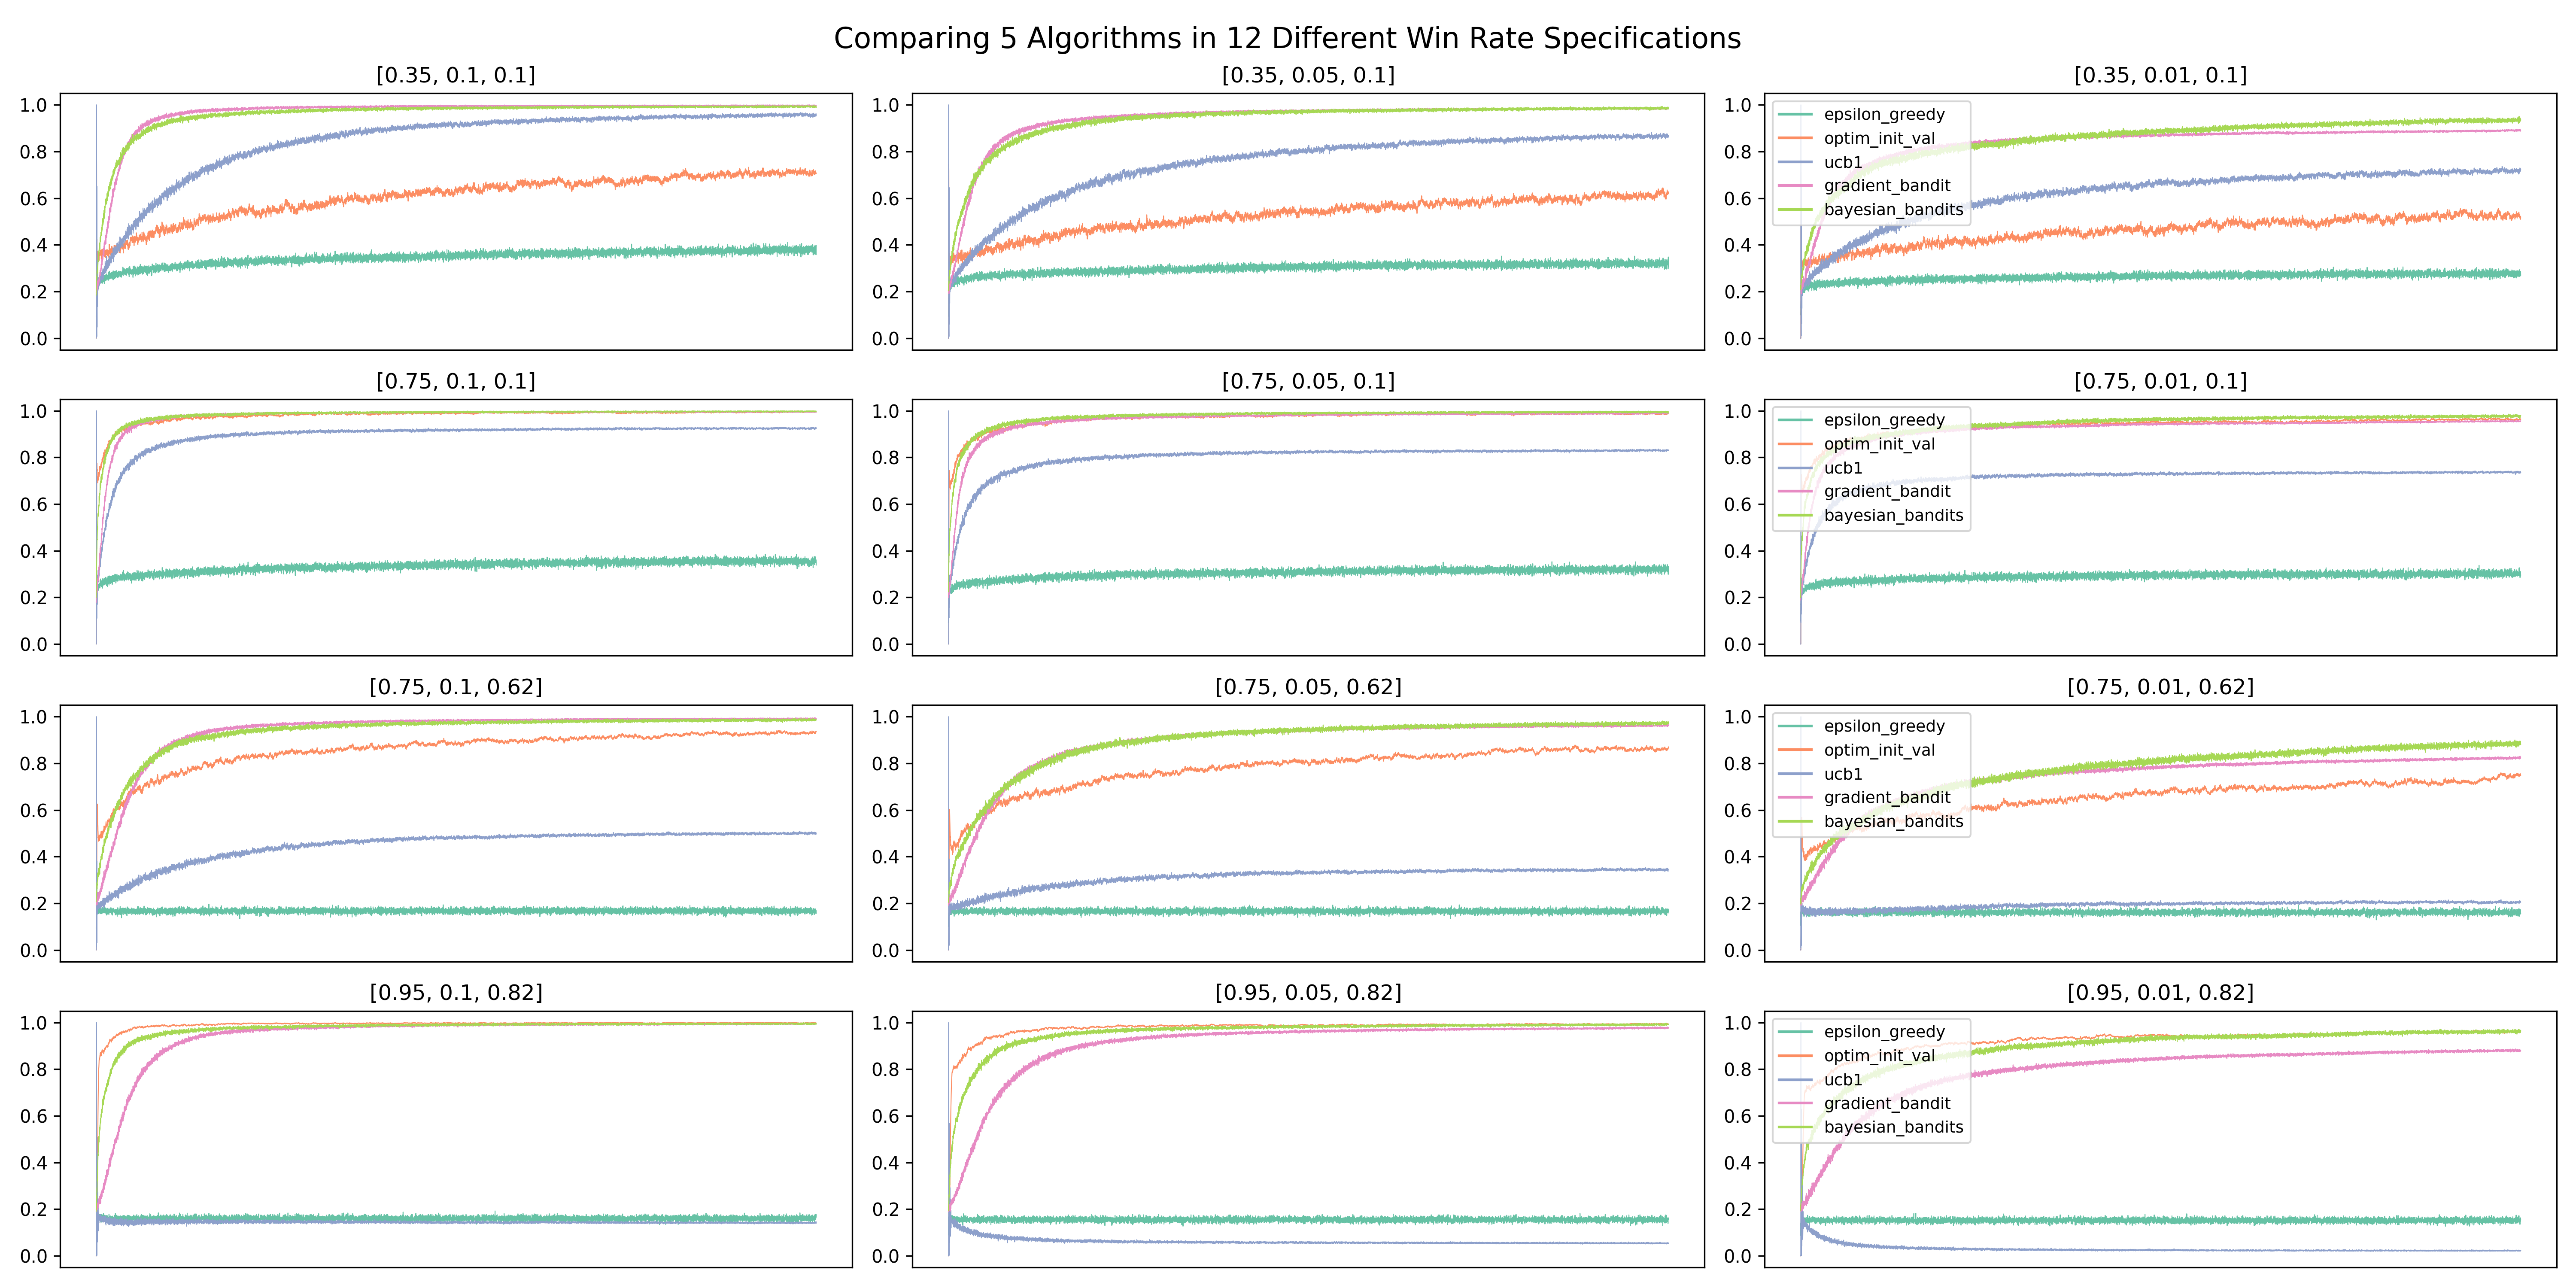
\includegraphics{images/comparison.png}
\caption{Comparison}
\end{figure}

Several results are worth mentioning:
1. \texttt{Thompson\ Sampling} and \texttt{Gradient\ Bandit} both do consistently well. \texttt{Thompson\ Sampling} has the best overall performance, picking the best bandit in over 90\% of the simulations at the end of 10,000 rounds. It also edged out \texttt{Gradient\ Bandit} when \texttt{p\_diff} is 0.01, which means there can be a close second-best bandit;
2. The \texttt{Epsilon\ Greedy} algorithm performs consistently regardless of win rate settings, but at a poor 20\% success rate at picking the best bandit. This may be partly due to a relatively high value of epsilon at 0.5;
3. The algorithm that is the most sensitive to win rate settings is \texttt{UCB1}. When the win rate of the best bandit is at 0.95, \texttt{UCB1}'s performance can be puzzling. In part, it may be a the result of a relatively high \texttt{c} value, since the default is 1. Intuitively, when the best bandit has a win rate of 0.95, and especially when there exists a close second-best, the ``bonus'' that \texttt{UCB1} can give to a bandit is small. After all, the win rate is not to be exceeding 1. As a result, \texttt{UCB1} has a hard time distinguishing between the best bandits and others that are almost as good. It should be noted that \texttt{UCB} (not \texttt{UCB1}) has the best performance in the testbed in Sutton and Barto (2020), but the authors also acknowledged that \texttt{UCB}'s application beyond the Multi-Armed Bandit problem is limited (in the context of reinforcement learning).

\hypertarget{summary-and-extensions}{%
\section{Summary and Extensions}\label{summary-and-extensions}}

In this article, I have introduced five algorithms that can be used in \emph{real-time} A/B Testing and Randomized Controlled Trials. Compared to traditional methods that often use Power Analysis to determine the minimum sample size, algorithms introduced in this article have one additional advantage: They can be easily extended to experiments with more than 2 choices/versions/bandits, as shown throughout the article.

The algorithms introduced in this article are known as algorithms for the \texttt{Multi-Armed\ Bandit} problem, which is considered as the simplest form of \textbf{reinforcement learning}. We will come back to more reinforcement learning algorithms and problems in later articles.

Two extensions of the \texttt{Multi-Armed\ Bandit} problem should be mentioned: \texttt{Non-stationary\ Bandit} and \texttt{Contextual\ Bandit}. Non-stationary Bandit is the situation in which that the win rates change over time. One particular algorithm that we introduced in this article is known to do badly in non-stationary bandit problems: \texttt{Optimistic\ Initial\ Values}. The reason is obvious. \texttt{Optimistic\ Initial\ Values} algorithm is designed to explore aggressively in the beginning. When the win rates change after this initial exploration stage has ended, it is hard for it to change course.

As the name suggested, \texttt{Contextual\ Bandit} means that there exists contextual information to be used when making a decision. In a simple example, a casino may have slot machines in different colors, and the colors are not random: the green machines have higher win rates than the red ones. A new player would not know that information at first, but as time goes on and if the player has explored enough, it is possible to figure out the \emph{association} between color and win rate, and hence decisions are made accordingly. This is also why \texttt{Contextual\ Bandit} is also known as \texttt{Associative\ Search}. We will come back to this in another article, since \texttt{Contextual\ Bandit} algorithms can be used in regression problems.

(Visit my GitHub for the latest Python scripts: \url{https://github.com/DataHurdler/Econ-ML/tree/main/Multi-Arm\%20Bandits})

\hypertarget{references}{%
\section{References}\label{references}}

\begin{itemize}
\tightlist
\item
  \url{https://www.udemy.com/course/bayesian-machine-learning-in-python-ab-testing/}
\item
  \url{http://incompleteideas.net/book/the-book-2nd.html} (Chapter 2)
\item
  \url{https://en.m.wikipedia.org/wiki/Multi-armed_bandit}
\item
  \url{https://www.tensorflow.org/agents/tutorials/intro_bandit}
\end{itemize}

\hypertarget{discrete-choice-classification-and-tree-based-ensemble-algorithms}{%
\chapter{Discrete Choice, Classification, and Tree-Based Ensemble Algorithms}\label{discrete-choice-classification-and-tree-based-ensemble-algorithms}}

\hypertarget{introduction-1}{%
\section{Introduction}\label{introduction-1}}

Suppose you are the owner of an e-commerce website that sells a musical instrument in 5 sizes: soprano, alto, tenor, bass, and contrabass. You are now considering to open up some physical stores. With physical stores, you need to make more careful inventory decisions. Based on your past experience in shipping out your instruments, you are convinced that different communities can have different tastes toward different sizes. And you want to make inventory decisions accordingly.

If the stake for a musical store is too small, consider the classic discrete choice example: automobiles. Ultimately, we want to understand the question of ``who buys what.'' This can inform many business decisions, not only inventory, since the aggregation of individuals tells us the demand of a product in a market. Discrete choice is different from decisions about ``how much,'' for example, do I exercise 15 minutes or 25 minutes tonight?

In economics and social sciences, the popular approaches are ``top-down'': it starts with a understanding of the data-generating process and some assumptions. Logit and Probit are two widely used models in economics. If the error term is believed to follow a logistic distribution, then use the logit model or logistic regression. If the error term is believed to follow a normal distribution, then use the probit model. If there is nested structure, then use nested-logit. And so on.

This is fine, since the focus of economics and social sciences is hypothesis testing and to understand mechanisms. On the contrary, the machine learning approach is \emph{bottom-up}: it cares about making good predictions. In a way, the economics ``top-down'' approach of discrete choice modeling cares much more about ``bias'' whereas the machine learning approach considers the bias-variance tradeoff more holistically.

\hypertarget{the-bias-variance-tradeoff}{%
\section{The Bias-Variance Tradeoff}\label{the-bias-variance-tradeoff}}

Let's begin with \emph{Variance}. A model with a high variance is sensitive to the \emph{training} data and can capture the fine details in the training data. However, such model is usually difficult to generalize. On the one hand, the \emph{test} data, or the data that the model is actually applied to, may lack the fine detail presented in the training data. On the other hand, those fine details may not be as important in the actual data as compared to the training data.

A model that can capture fine details is almost guaranteed to have low \emph{bias}. A model with low bias is one that explains the known, or training, data well. In order to predict, we need our machine learning model to learn from known data. A model with high bias can rarely predict well.

While models with low bias \emph{and} low variance do exist, they are rare. Since a model with high bias rarely works well, lowering bias is often considered the first-order task. One way to do so is using models, or specifying hyperparameters of a model, such that more fine details in the data are taken in to consideration. By doing so, higher variance is introduced. And hence the trade off.

Consider the following example: a zoo wants to build a machine learning algorithm to detect penguin species and deploy it on their smart phone application. Let's say all that the zoo and its users care about is to tell apart King, Magellanic, and Macaroni penguins. The zoo's staffs and data scientists took hundreds of photos of penguins in their aquarium, split the penguins into training and test datasets, as how tasks like this are usually performed, and built the machine learning model. In their test, with photos that they have set aside earlier, they find that the algorithm is able to identify the penguins correctly 98\% of the time.

However, when their users use the algorithm to identify penguins in other zoos, the algorithm fails miserably. Why? It turns out that the machine learning algorithm was not learning to identify penguins by their different features such as head, neck, and tails. Instead, the algorithm identifies the different species of penguins by the tag on their wings: blue is for King penguin, red for Magellanic, and yellow for Macaroni. These are the colors used by the zoo who developed the algorithm, but different zoos have different tags. As a result, this algorithm, which has low bias but high variance, is unable to predict or detect the species of penguins outside of the zoo where photos for developing the machine learning model were taken.

As we will see next, tree-based algorithms are extremely prone to high variance, or \emph{over-fitting}.

\hypertarget{decision-tree}{%
\section{Decision Tree}\label{decision-tree}}

Let's first talk about the basic decision tree algorithm. Because we will be using \href{https://scikit-learn.org/stable/}{scikit-learn} for \texttt{Python} implementation in this chapter, I am using notations and languages similar to that in scikit-learn's documentations. It should be mentioned at the outset that this is not a comprehensive lecture on the decision tree algorithm. You can easily find more in-depth discussions in books such as \href{https://www.statlearning.com/}{An Introduction to Statistical Learning} and \href{https://hastie.su.domains/ElemStatLearn/}{The Elements of Statistical Learning}, or other online learning sources. Our focuses here are aspects of the decision tree algorithm that matter the most for the understanding of the ensemble methods and their applications in economics and business.

The simplest way to think about a decision tree algorithm is to consider a flow-chart, especially one that is for diagnostic purposes. Instead of someone building a flow-chart from intuition or experience, we feed data into the computer and the decision tree algorithm would build a flow-chart to explain the data. For example, if we know some characteristics of consumers of the music store, and want to know who is more likely to buy the smaller size instruments, a flow-chart, built by the decision tree algorithm, may look like this:
* Is the customer under 30?
* Yes: is the customer female?
* Yes: has the customer played any instrument before?
* Yes: the customer has a 90\% chance buying a smaller instruments
* No: the customer has 15\% chance buying a smaller instruments
* No: is the customer married?
* Yes: the customer has a 5\% chance buying a smaller instruments
* No: the customer has 92\% chance buying a smaller instruments
* No: is the customer under 50?
* Yes: the customer has a 10\% chance buying a smaller instruments
* No: has the customer played any instrument before?
* Yes: the customer has a 100\% chance buying a smaller instruments
* No: the customer has a 20\% chance buying a smaller instruments

You can see several basic elements of a decision tree algorithm from the above example:

\begin{enumerate}
\def\labelenumi{\arabic{enumi}.}
\tightlist
\item
  As expected, the tree algorithm resulted in a hierarchical structure that can be easily represented by a tree diagram;
\item
  The tree structure does not need to be symmetrical. For example, when the answer to ``is the customer under 50'' is a ``yes'', the branch stopped, resulted in a shorter branch compared to the rest of the tree;
\item
  You may use the same feature more than once. In this example, the question ``has the customer played any instrument before'' has appeared twice. Also there are two splits based on two different age cutoffs;
\item
  You can use both categorical and numerical features. In this example, age is numerical, whereas all other features are categorical;
\item
  It is accustomed to split to only two branches at each node. If you want three branches, you can do it at the next node: two branches at the first node, then one or both of the next nodes split into another 2 branches.
\end{enumerate}

There are other elements of a decision tree algorithm that you can not observe directly from this example but are very important. We will examine these in more details below.

\hypertarget{split-criterion}{%
\section{Split Criterion}\label{split-criterion}}

At each node, the split must be based on some criterion. The commonly used criteria are \textbf{Gini impurity} and \textbf{Entropy} (or \textbf{Log-loss}). According to the scikit-learn documentation, let

\[p_{mk}=\frac{1}{n_m}\sum_{y\in Q_m}{I(y=k)}\]

denote the proportion of class \(k\) observations in node \(m\), where \(Q_m\) is the data at node \(m\), \(n_m\) is the sample size at node \(m\), and \(I(\cdot)\) returns 1 when \(y=k\) and 0 otherwise. Then, the \textbf{Gini impurity} is given by:

\[H(Q_m)=\sum_{k}{p_{mk}(1-p_{mk})}\]

whereas \textbf{Entropy} is given by:

\[H(Q_m)=-\sum_{k}{p_{mk}\log{(p_{mk})}}\]

At each node \(m\), a \texttt{candidate} is defined by the combination of feature and threshold. For example, in the above example, for the question ``Is the customer under 30,'' the feature is age and the threshold is 30. Let \(\theta\) denote a candidate, which splits \(Q_m\) into two partitions: \(Q_m^{\text{left}}\) and \(Q_m^{\text{right}}\). Then the quality of a split with \(\theta\) is computed as the weighted average of the criterion function \(H(Q_m)\):

\[G(Q_m, \theta) = \frac{n_m^{\text{left}}}{n_m}H(Q_m^{\text{left}}(\theta)) + \frac{n_m^{\text{right}}}{n_m}H(Q_m^{\text{right}}(\theta))\]

The objective of the decision tree algorithm is to find the candidate that minimizes the quality at each \(m\):

\[\theta^{*} = \underset{\theta}{\operatorname{argmin}}{G(Q_m, \theta)}\]

It is straightforward to see that, from either the \textbf{Gini impurity} or the \textbf{Entropy} criterion function, the unconstrained minimum of \(G(Q_m, \theta)\) is achieved at \(p_{mk}=0\) or \(p_{mk}=1\), i.e., when the result of the split consists of a single class.

Before we move on, here is a quick remark: while there exists a global optimum for building a decision tree, where the quality function is minimized for the \emph{whole} tree, the computation of such algorithm is too complex. As a result, practical decision tree algorithms resolve to using \emph{local} optima at each node as described above.

\hypertarget{pruning}{%
\section{Pruning}\label{pruning}}

If achieving a ``pure'' branch, where there remains observations from a single class after a split, minimizes the quality function \(G(Q_m, \theta)\), then why did we not achieve that ``pure'' state in the illustrative example with the music store? There are two main reasons. First, we may not have enough features. Imagine you have two individuals in your data set, one bought a small instrument and the other bought a large instrument. These two individuals are almost identical: the only difference is in their eye colors. If ``eye color'' is not one of the features captured in your data set, you will have no way to distinguish these two individuals. On the other hand, imagine we know \emph{everything} about each and every individual, then it is almost guaranteed that you can find a ``perfect'' tree, such that there is a single class of individuals at each end node. Such ``perfect'' tree may not be unique. At the extreme, imagine a tree such that each end node represents a single individual.

The second reason is something we have discussed: the Bias-Variance Tradeoff. Because the ultimate goal is to predict, fitting a ``perfect'' tree can result in too high of a variance. Continued with the previous example, your ability to build a perfect tree would totally depend on whether you have ``eye color'' as a feature in your data set. That means that your algorithm is too sensitive to one particular feature - if this feature does not exist, your algorithm would fail to build a ``perfect'' tree (assuming that was the goal). Or, if this feature is somehow absent or incorrect in the data set you are predicting on, your algorithm would have a breakdown.

This is why a decision tree needs to be pruned. This is often done by specifying two hyperparameters in the decision tree algorithm in scikit-learn: the maximum depth of the tree (\texttt{max\_depth}) and the minimum number of samples required to split (\texttt{min\_samples\_split}). Without going into the technical details, we can intuitively understand that both of these restrictions can prevent us from splitting the tree to the extreme case such that each end node represents an individual. In other words, they restrict the growth of a tree.

The caveat of a single decision tree algorithm is obvious: it can easily suffer from either high bias or high variance, especially the latter. This is why ensemble methods such as \textbf{bagging} and \textbf{boosting} were introduced. In practice, a single decision tree is rarely used as the ``finale'' model. It is often used as a demonstrative example.

\hypertarget{bagging-and-random-forest}{%
\section{Bagging and Random Forest}\label{bagging-and-random-forest}}

\texttt{Bagging} is one of two ensemble methods based on the decision tree algorithm. \texttt{Bagging} is short for \emph{bootstrap aggregation}, which explains what bagging algorithms do: select random subsets from the training data set, fit the decision tree algorithm on each subset, and aggregate to get the prediction. There are several variations of \texttt{Bagging} algorithms depending on how random samples are drawn:

\begin{enumerate}
\def\labelenumi{\arabic{enumi}.}
\tightlist
\item
  When random subsets were drawn with replacement (bootstrap), the algorithm is known as \texttt{Bagging} (Breiman, 1996)
\item
  When random subsets were drawn without replacement, the algorithm is known as \texttt{Pasting} (Breiman, 1999)
\item
  When random subsets are drawn based on features rather than individuals, the algorithm is known as \texttt{Subspaces} (Ho, 1998)
\item
  When random subsets are drawn based on both features and individuals, the algorithm is known as \texttt{Random\ Patches} (Louppe and Geurts, 2012)
\item
  When random subsets were drawn with replacement (bootstrap) \emph{and} at each split, a random subset of features is chosen, the algorithm is known as \texttt{Random\ Forest} (Breiman, 2001)
\end{enumerate}

In scikit-learn, the first four algorithms are implemented in \texttt{BaggingClassifier} whereas \texttt{Random\ Forest} is implemented in \texttt{RandomForestClassifier}.

In bagging algorithms, the ``aggregation'' of results during prediction is usually taken by votes. For example, suppose you have fit your data with the \texttt{Random\ Forest} algorithm with 1,000 trees, and now you want to know whether a new customer is going to buy a small or a large instrument. When the algorithm considers the first split, it will look at all 1,000 trees and see which candidate was used the most. Suppose ``Is the customer under 30'' appeared in 800 of the trees, then the algorithm would split according to \texttt{age=30}. And so, at each split, the algorithm would take a tally from the 1,000 individual trees and act accordingly, just like how one would look at a flow-chart to determine actions.

While a \texttt{Bagging} algorithm helps to reduce bias, the main benefit of bootstrapping is to reduce variance. The \texttt{Random\ Forest} algorithm, for example, is able to reduce variance in two ways: First, bootstrapping random samples is equivalent to consider many different scenarios. Not only does this mean that the algorithm is less reliant on a particular scenario (the whole training data set), it also makes it possible that one or some of the random scenarios may be similar to the ``future,'' i.e., the environment that the algorithm needs to make prediction on. Second, by considering a random set of features at each split, the algorithm is less reliant on certain features, and is hence resilient to ``future'' cases where certain features may be missing or have errors.

\hypertarget{boosting-and-adaboost}{%
\section{Boosting and AdaBoost}\label{boosting-and-adaboost}}

While the main benefit of \texttt{Bagging} is in reducing variance, the main benefit of \texttt{Boosting} is to reduce bias, while maintaining a reasonably low variance. Boosting is able to maintain a low variance because, like Bagging, it also fits many trees. Unlike Bagging, which builds the trees in parallel, Boosting builds them sequentially.

The basic idean of boosting is to have incremental (small/``weak'') improvements from the previous model, which is why the learning algorithms are built sequentially. This idea can be applied to all types of algorithms. In the context of decision tree, a boosting algorithm can be demonstrated by the following pseudocode:

\begin{verbatim}
Step 1: Build a simple decision tree (weak learner)
Step 2: Loop:
            Minimize weighted error
\end{verbatim}

Currently, there are three popular types of tree-based boosting algorithms: \texttt{AdaBoost}, \texttt{Gradient\ Boosting}, and \texttt{XGBoost}. The different algorithms are different in how they \emph{boost}, i.e., how to implement Step 2.

\texttt{AdaBoost} was introduced by Freund and Schapire (1995). It is short for \emph{Ada}ptive \emph{Boost}ing. \texttt{AdaBoost} implements boosting by changing the weights of observations. That is, by making some observations/individuals more important than the other. In a training data set with \(N\) individuals, the algorithm begins by weighting each individual the same: at a weight of \(1/N\). Then it fits a simple decision tree model and makes predictions. Inevitably, it makes better decision for some individuals than the other. The algorithm then increases the weight for individuals that it did not make correct/good predictions on in the first model. Effectively, this asks the next decision tree algorithm to focus more on these individuals that it has failed to understand in the first tree. And this process continues until a stopping rule is reached. A stopping rule may be, for example, ``\textbf{stops} when 98\% of the individuals are correctly predicted''.

It is straightforward to see that a boosting algorithm lowers bias. But was it often able to main a low \emph{variance} too? It was able to do so because a boosting algorithm effectively builds different trees at each iteration. When making predictions, it takes a weighted average of the models. Some mathematical details may be helpful.

Let \(w_{ij}\) denote the weight of individual \(i\) in stage/iteration \(j\). In the beginning of the algorithm, we have \(w_{i1}=1/N\) for all \(i\) where \(N\) is the the total number of individuals. After the first weak tree is built, we can calculate the error/misclassification rate of stage \(j\) as

\[e_j = \frac{\sum_{N}{w_{ij}\times I_{ij}(\text{incorrect})}}{\sum_{N}{w_{ij}}}\]

where \(I_{ij}(\text{incorrect})\) equals 1 if the prediction for individual \(i\) is incorrect in stage \(j\) and 0 otherwise. We can then calculate the \emph{stage value} of model \(j\):

\[v_j = \frac{1}{2}\log\left(\frac{1-e_j}{e_j}\right)\]

The stage value is used both in updating \(w_{ij+1}\), i.e., the weight of individual \(i\) in the next stage, and to act as the weight of model \(j\) when prediction is computed. To update the weight for the next stage/model, we have

\[w_{ij+1} = w_{ij} \times \exp{(v_j \times I_{ij}(\hat{y}_{ij}=y_i))}\]

where \(\hat{y}_{ij}\) is the prediction for individual \(i\) in stage \(j\), and \(y_i\) is the true label for individual \(i\). For binary classification, it is conventional to expression \(\hat{y}_{ij}\) and \(y_i\) as 1 and -1, so that the above equation can be simplified into

\[w_{ij+1} = w_{ij} \times \exp{(v_j \times \hat{y}_{ij}\times y_i)}\]

At each stage \(j(>1)\), the \texttt{AdaBoost} algorithm aims to minimize \(e_j\).

To compute the overall/final prediction, let \(\hat{y}_{ij}\) denote the prediction of model/stage \(j\) for individual \(i\), then the predicted value is calculated by:

\[\hat{y}_{i} = \sum_{J}{\hat{y}_{ij} \times v_j}\]

where \(J\) is the total number of stages.

\hypertarget{gradient-boosting-and-xgboost}{%
\section{Gradient Boosting and XGBoost}\label{gradient-boosting-and-xgboost}}

\texttt{Gradient\ Boosting} (Friedman, 2001) is another approach to boost. Instead of updating the weight after each stage/model, Gradient Boosting aims to minimize a loss function, using method such as gradient decent. The default loss function in scikit-learn, which is also the most common in practice, is the binomial deviance:

\[L_j = -2\sum_{N}{y_i\log{(\hat{p}_{ij})} + (1-y_i)\log{(1-\hat{p}_{ij})}}\]

where \(N\) is the number of individuals, \(y_i\) is the true label for individual \(i\), and \(\hat{p}_{ij}\) is the predicted probability that individual \(i\) at stage \(j\) having a label of \(y\), and is given by the softmax (logistic) function when log-loss is specified:

\[\hat{p}_{ij} = \frac{\exp{(F_j(x_i))}}{1+\exp{(F_j(x_i))}}\]

where \(F_j(x_i)\) is a numerical predicted value for individual \(i\) by regressor \(F_j(x)\). Here, \(F_j(x)\) is the aggregated regressor in stage \(j\), which is given by

\[F_j(x) = F_{j-1}(x) + h_j(x)\]

where \(h_j(x)\) is the weak learner/regressor at stage \(j\) that minimizes \(L_j\). Substituting \(F_M(x)\), the final regressor, into the above formula for \(\hat{p}_{ij}\) gives the overall prediction of the Gradient Boosting model.

Finally, using first-order Taylor approximation, it can be shown that minimizing \(L_j\) is approximately equivalent to predicting the negative gradient of the samples, where the negative gradient for individual \(i\) is given by

\[-g_i = -\left[\frac{\partial l_{ij-1}}{\partial F_{j-1}(x_i)}\right]\]

where \(l_{ij-1}\) is the term inside the summation in \(L_j\) (but lagged one stage):

\[l_{ij-1} = y_i\log{(\hat{p}_{ij-1})} + (1-y_i)\log{(1-\hat{p}_{ij-1})}\]

In other words, while the basic decision tree algorithm aims to predict the true classes, usually represented by 0's and 1's, \texttt{Gradient\ Boosting} aims to predict a numerical value which is the gradient. This means that, at each stage, Gradient Boosting is a regression problem rather than a classification problem. Predicting the gradient allows the algorithm to utilize many well developed methods for such task, for example, the Nelder-Mead method or simple grid search.

The discussion above focused on binary classification, which requires a single tree to be built in each stage. In multiclass classification, \(K\) trees would be built for \(K\) classes. For example, if \texttt{Gradient\ Boosting} is used to identify the 26 English alphabets, 26 trees are built and fitted in each stage.

\texttt{XGBoost} was introduced by Tianqi Chen in 2014. It is short for ``e\emph{X}treme \emph{G}radient \emph{Boost}ing''. Instead of gradient decent, \texttt{XGBoost} implements \href{https://en.wikipedia.org/wiki/Newton\%27s_method}{Newton's Method}, which is computationally much more demanding than gradient decent and requires a second-order Taylor approximation (instead of first-order as in \texttt{Gradient\ Boosting}). Due to this, in addition to \textbf{Gradients}, \texttt{XGBoost} also calculates the \textbf{Hessians}, which are a set of second-order derivatives (whereas gradients are the first-order derivatives).

\texttt{Python} library \texttt{xgboost} implements \texttt{XGBoost} and can easily be integrated with \texttt{scikit-learn}, which is the library we use to implement all algorithms covered in this chapter.

\hypertarget{python-implementation-with-scikit-learn}{%
\section{Python Implementation with scikit-learn}\label{python-implementation-with-scikit-learn}}

As we have done in other chapters, we will first generate a data set, then fit the data with various algorithms. After we have fitted the models, we will print out some basic performance metrics, chief among which is the \texttt{confusion\ matrix} and conduct a cross validation exercise.

The algorithms we will consider include:
* Logistic regression
* Decision tree classifier
* Random forest classifier
* Adaboost classifier
* Gradient boosting classifier
* XGBoost

Even though logistic regression is not covered in this chapter, I included it in the Python implementation for comparison purposes. Although not necessary, I use a Python class in this implementation. Here is the full script:

\begin{Shaded}
\begin{Highlighting}[]
\ImportTok{import}\NormalTok{ random}
\ImportTok{import}\NormalTok{ string}
\ImportTok{import}\NormalTok{ numpy }\ImportTok{as}\NormalTok{ np}
\ImportTok{import}\NormalTok{ pandas }\ImportTok{as}\NormalTok{ pd}
\ImportTok{import}\NormalTok{ matplotlib.pyplot }\ImportTok{as}\NormalTok{ plt}
\ImportTok{from}\NormalTok{ sklearn.cluster }\ImportTok{import}\NormalTok{ KMeans}
\ImportTok{from}\NormalTok{ sklearn.model\_selection }\ImportTok{import}\NormalTok{ train\_test\_split, cross\_val\_score}
\ImportTok{from}\NormalTok{ sklearn.linear\_model }\ImportTok{import}\NormalTok{ LogisticRegression}
\ImportTok{from}\NormalTok{ sklearn.tree }\ImportTok{import}\NormalTok{ DecisionTreeClassifier}
\ImportTok{from}\NormalTok{ sklearn.ensemble }\ImportTok{import}\NormalTok{ RandomForestClassifier}
\ImportTok{from}\NormalTok{ sklearn.ensemble }\ImportTok{import}\NormalTok{ AdaBoostClassifier}
\ImportTok{from}\NormalTok{ sklearn.ensemble }\ImportTok{import}\NormalTok{ GradientBoostingClassifier}
\ImportTok{from}\NormalTok{ sklearn.metrics }\ImportTok{import}\NormalTok{ accuracy\_score, precision\_score, recall\_score, f1\_score}
\ImportTok{from}\NormalTok{ sklearn.metrics }\ImportTok{import}\NormalTok{ confusion\_matrix, ConfusionMatrixDisplay}
\ImportTok{import}\NormalTok{ xgboost}

\NormalTok{N\_GROUP }\OperatorTok{=} \DecValTok{5}
\NormalTok{N\_IND }\OperatorTok{=} \DecValTok{50000}
\NormalTok{N\_FEATURES }\OperatorTok{=} \DecValTok{10}


\KeywordTok{class}\NormalTok{ TreeModels:}
    \KeywordTok{def} \FunctionTok{\_\_init\_\_}\NormalTok{(}
            \VariableTok{self}\NormalTok{,}
\NormalTok{            n\_group: }\BuiltInTok{int} \OperatorTok{=} \DecValTok{5}\NormalTok{,}
\NormalTok{            n\_individuals: }\BuiltInTok{int} \OperatorTok{=} \DecValTok{10000}\NormalTok{,}
\NormalTok{            n\_num\_features: }\BuiltInTok{int} \OperatorTok{=} \DecValTok{10}\NormalTok{,}
\NormalTok{            numeric\_only: }\BuiltInTok{bool} \OperatorTok{=} \VariableTok{False}\NormalTok{,}
\NormalTok{    ):}
        \CommentTok{"""}
\CommentTok{        Initialize the TreeModels class.}

\CommentTok{        Args:}
\CommentTok{            n\_group (int): Number of groups. Default is 5.}
\CommentTok{            n\_individuals (int): Number of individuals. Default is 10000.}
\CommentTok{            n\_num\_features (int): Number of numerical features. Default is 10.}
\CommentTok{            numeric\_only (bool): Flag to indicate whether to use only numerical features. Default is False.}

\CommentTok{        Returns:}
\CommentTok{            None}
\CommentTok{        """}
        \BuiltInTok{print}\NormalTok{(}\SpecialStringTok{f\textquotesingle{}There are }\SpecialCharTok{\{}\NormalTok{n\_individuals}\SpecialCharTok{\}}\SpecialStringTok{ individuals.\textquotesingle{}}\NormalTok{)}
        \BuiltInTok{print}\NormalTok{(}\SpecialStringTok{f\textquotesingle{}There are }\SpecialCharTok{\{}\NormalTok{n\_group}\SpecialCharTok{\}}\SpecialStringTok{ choices.\textquotesingle{}}\NormalTok{)}
        \BuiltInTok{print}\NormalTok{(}\SpecialStringTok{f\textquotesingle{}There are }\SpecialCharTok{\{}\NormalTok{n\_num\_features}\SpecialCharTok{\}}\SpecialStringTok{ numerical features and 1 categorical feature.\textquotesingle{}}\NormalTok{)}

        \VariableTok{self}\NormalTok{.numeric\_only }\OperatorTok{=}\NormalTok{ numeric\_only}

        \CommentTok{\# Generate random numerical features and categorical feature}
        \VariableTok{self}\NormalTok{.num\_features }\OperatorTok{=}\NormalTok{ np.random.rand(n\_individuals, n\_num\_features }\OperatorTok{+} \DecValTok{2}\NormalTok{)}
\NormalTok{        cat\_list }\OperatorTok{=}\NormalTok{ random.choices(string.ascii\_uppercase, k}\OperatorTok{=}\DecValTok{6}\NormalTok{)}
        \VariableTok{self}\NormalTok{.cat\_features }\OperatorTok{=}\NormalTok{ np.random.choice(cat\_list, size}\OperatorTok{=}\NormalTok{(n\_individuals, }\DecValTok{1}\NormalTok{))}

        \CommentTok{\# Create a DataFrame with numerical features and one{-}hot encoded categorical feature}
        \VariableTok{self}\NormalTok{.df }\OperatorTok{=}\NormalTok{ pd.DataFrame(}\VariableTok{self}\NormalTok{.num\_features[:, :}\OperatorTok{{-}}\DecValTok{2}\NormalTok{])}
        \VariableTok{self}\NormalTok{.df[}\StringTok{\textquotesingle{}cat\_features\textquotesingle{}}\NormalTok{] }\OperatorTok{=} \VariableTok{self}\NormalTok{.cat\_features}
        \VariableTok{self}\NormalTok{.df }\OperatorTok{=}\NormalTok{ pd.get\_dummies(}\VariableTok{self}\NormalTok{.df, prefix}\OperatorTok{=}\NormalTok{[}\StringTok{\textquotesingle{}cat\textquotesingle{}}\NormalTok{])}
        \VariableTok{self}\NormalTok{.df.columns }\OperatorTok{=} \VariableTok{self}\NormalTok{.df.columns.astype(}\BuiltInTok{str}\NormalTok{)}

        \ControlFlowTok{if}\NormalTok{ numeric\_only:}
            \CommentTok{\# Cluster the data based on numerical features only}
            \CommentTok{\# Logistic regression performs the best in this condition}
\NormalTok{            kmeans }\OperatorTok{=}\NormalTok{ KMeans(n\_clusters}\OperatorTok{=}\NormalTok{n\_group, n\_init}\OperatorTok{=}\StringTok{"auto"}\NormalTok{).fit(}\VariableTok{self}\NormalTok{.num\_features)}
            \VariableTok{self}\NormalTok{.df[}\StringTok{\textquotesingle{}target\textquotesingle{}}\NormalTok{] }\OperatorTok{=}\NormalTok{ kmeans.labels\_}
        \ControlFlowTok{else}\NormalTok{:}
            \CommentTok{\# Cluster the data based on both numerical and categorical features}
\NormalTok{            cat\_columns }\OperatorTok{=} \VariableTok{self}\NormalTok{.df.}\BuiltInTok{filter}\NormalTok{(like}\OperatorTok{=}\StringTok{\textquotesingle{}cat\textquotesingle{}}\NormalTok{)}
\NormalTok{            kmeans1 }\OperatorTok{=}\NormalTok{ KMeans(n\_clusters}\OperatorTok{=}\NormalTok{n\_group, n\_init}\OperatorTok{=}\StringTok{"auto"}\NormalTok{).fit(cat\_columns)}
\NormalTok{            kmeans2 }\OperatorTok{=}\NormalTok{ KMeans(n\_clusters}\OperatorTok{=}\NormalTok{n\_group, n\_init}\OperatorTok{=}\StringTok{"auto"}\NormalTok{).fit(}\VariableTok{self}\NormalTok{.num\_features)}
            \VariableTok{self}\NormalTok{.df[}\StringTok{\textquotesingle{}target\textquotesingle{}}\NormalTok{] }\OperatorTok{=}\NormalTok{ np.floor((kmeans1.labels\_ }\OperatorTok{+}\NormalTok{ kmeans2.labels\_) }\OperatorTok{/} \DecValTok{2}\NormalTok{)}

        \CommentTok{\# Add some random noise to the numerical features}
\NormalTok{        numerical\_columns }\OperatorTok{=}\NormalTok{ [}\BuiltInTok{str}\NormalTok{(i) }\ControlFlowTok{for}\NormalTok{ i }\KeywordTok{in} \BuiltInTok{range}\NormalTok{(n\_num\_features)]}
        \ControlFlowTok{for}\NormalTok{ column }\KeywordTok{in}\NormalTok{ numerical\_columns:}
            \VariableTok{self}\NormalTok{.df[column] }\OperatorTok{=} \VariableTok{self}\NormalTok{.df[column] }\OperatorTok{+}\NormalTok{ random.gauss(mu}\OperatorTok{=}\DecValTok{0}\NormalTok{, sigma}\OperatorTok{=}\DecValTok{3}\NormalTok{)}

        \CommentTok{\# Split the data into training and testing sets}
        \VariableTok{self}\NormalTok{.X }\OperatorTok{=} \VariableTok{self}\NormalTok{.df.drop(columns}\OperatorTok{=}\NormalTok{[}\StringTok{\textquotesingle{}target\textquotesingle{}}\NormalTok{])}
        \VariableTok{self}\NormalTok{.y }\OperatorTok{=} \VariableTok{self}\NormalTok{.df[}\StringTok{\textquotesingle{}target\textquotesingle{}}\NormalTok{]}
        \VariableTok{self}\NormalTok{.X\_train, }\VariableTok{self}\NormalTok{.X\_test, }\VariableTok{self}\NormalTok{.y\_train, }\VariableTok{self}\NormalTok{.y\_test }\OperatorTok{=}\NormalTok{ train\_test\_split(}
            \VariableTok{self}\NormalTok{.X, }\VariableTok{self}\NormalTok{.y, test\_size}\OperatorTok{=}\FloatTok{0.3}\NormalTok{, random\_state}\OperatorTok{=}\DecValTok{42}\NormalTok{)}

        \CommentTok{\# Initialize the y\_pred variable}
        \VariableTok{self}\NormalTok{.y\_pred }\OperatorTok{=}\NormalTok{ np.empty([n\_individuals, }\DecValTok{1}\NormalTok{])}

        \CommentTok{\# Initialize a dictionary to save results}
        \VariableTok{self}\NormalTok{.results }\OperatorTok{=} \BuiltInTok{dict}\NormalTok{()}

    \KeywordTok{def}\NormalTok{ show\_results(}\VariableTok{self}\NormalTok{, clf, clf\_name, print\_flag}\OperatorTok{=}\VariableTok{False}\NormalTok{, plot\_flag}\OperatorTok{=}\VariableTok{True}\NormalTok{):}
        \CommentTok{"""}
\CommentTok{        Train and evaluate a classifier.}

\CommentTok{        Args:}
\CommentTok{            clf: Classifier object.}
\CommentTok{            clf\_name (str): Name of the classifier.}
\CommentTok{            print\_flag (bool): Whether to print results. Default is False.}
\CommentTok{            plot\_flag (bool): Whether to draw CM plots and save them. Default is True.}

\CommentTok{        Returns:}
\CommentTok{            None}
\CommentTok{        """}
        \BuiltInTok{print}\NormalTok{(clf\_name)}
\NormalTok{        clf.fit(}\VariableTok{self}\NormalTok{.X\_train, }\VariableTok{self}\NormalTok{.y\_train)}
        \VariableTok{self}\NormalTok{.y\_pred }\OperatorTok{=}\NormalTok{ clf.predict(}\VariableTok{self}\NormalTok{.X\_test)}

        \CommentTok{\# Calculate evaluation metrics}
\NormalTok{        train\_acc }\OperatorTok{=}\NormalTok{ clf.score(}\VariableTok{self}\NormalTok{.X\_train, }\VariableTok{self}\NormalTok{.y\_train)}
\NormalTok{        acc }\OperatorTok{=}\NormalTok{ accuracy\_score(}\VariableTok{self}\NormalTok{.y\_test, }\VariableTok{self}\NormalTok{.y\_pred)}
\NormalTok{        precision }\OperatorTok{=}\NormalTok{ precision\_score(}\VariableTok{self}\NormalTok{.y\_test, }\VariableTok{self}\NormalTok{.y\_pred, average}\OperatorTok{=}\StringTok{\textquotesingle{}weighted\textquotesingle{}}\NormalTok{)}
\NormalTok{        recall }\OperatorTok{=}\NormalTok{ recall\_score(}\VariableTok{self}\NormalTok{.y\_test, }\VariableTok{self}\NormalTok{.y\_pred, average}\OperatorTok{=}\StringTok{\textquotesingle{}weighted\textquotesingle{}}\NormalTok{)}
\NormalTok{        f1 }\OperatorTok{=}\NormalTok{ f1\_score(}\VariableTok{self}\NormalTok{.y\_test, }\VariableTok{self}\NormalTok{.y\_pred, average}\OperatorTok{=}\StringTok{\textquotesingle{}weighted\textquotesingle{}}\NormalTok{)}

        \CommentTok{\# Perform cross{-}validation and print the average score}
\NormalTok{        cv\_score }\OperatorTok{=}\NormalTok{ cross\_val\_score(clf, }\VariableTok{self}\NormalTok{.X, }\VariableTok{self}\NormalTok{.y, cv}\OperatorTok{=}\DecValTok{10}\NormalTok{)}

        \ControlFlowTok{if}\NormalTok{ print\_flag:}
            \ControlFlowTok{if} \BuiltInTok{isinstance}\NormalTok{(clf, LogisticRegression):}
                \BuiltInTok{print}\NormalTok{(}\SpecialStringTok{f\textquotesingle{}Coefficients: }\SpecialCharTok{\{}\NormalTok{clf}\SpecialCharTok{.}\NormalTok{coef\_}\SpecialCharTok{\}}\SpecialStringTok{\textquotesingle{}}\NormalTok{)}
            \ControlFlowTok{else}\NormalTok{:}
                \BuiltInTok{print}\NormalTok{(}\SpecialStringTok{f\textquotesingle{}Feature Importance: }\SpecialCharTok{\{}\NormalTok{clf}\SpecialCharTok{.}\NormalTok{feature\_importances\_}\SpecialCharTok{\}}\SpecialStringTok{\textquotesingle{}}\NormalTok{)}
            \BuiltInTok{print}\NormalTok{(}\SpecialStringTok{f\textquotesingle{}Training accuracy: }\SpecialCharTok{\{}\NormalTok{train\_acc}\SpecialCharTok{:.4f\}}\SpecialStringTok{\textquotesingle{}}\NormalTok{)}
            \BuiltInTok{print}\NormalTok{(}\SpecialStringTok{f\textquotesingle{}Test accuracy: }\SpecialCharTok{\{}\NormalTok{acc}\SpecialCharTok{:.4f\}}\SpecialStringTok{\textquotesingle{}}\NormalTok{)}
            \BuiltInTok{print}\NormalTok{(}\SpecialStringTok{f\textquotesingle{}Test precision: }\SpecialCharTok{\{}\NormalTok{precision}\SpecialCharTok{:.4f\}}\SpecialStringTok{\textquotesingle{}}\NormalTok{)}
            \BuiltInTok{print}\NormalTok{(}\SpecialStringTok{f\textquotesingle{}Test recall: }\SpecialCharTok{\{}\NormalTok{recall}\SpecialCharTok{:.4f\}}\SpecialStringTok{\textquotesingle{}}\NormalTok{)}
            \BuiltInTok{print}\NormalTok{(}\SpecialStringTok{f\textquotesingle{}Test F1 score: }\SpecialCharTok{\{}\NormalTok{f1}\SpecialCharTok{:.4f\}}\SpecialStringTok{\textquotesingle{}}\NormalTok{)}
            \BuiltInTok{print}\NormalTok{(}\SpecialStringTok{f\textquotesingle{}Average Cross Validation: }\SpecialCharTok{\{}\NormalTok{np}\SpecialCharTok{.}\NormalTok{mean(cv\_score)}\SpecialCharTok{\}}\SpecialStringTok{\textquotesingle{}}\NormalTok{)}

        \ControlFlowTok{if}\NormalTok{ plot\_flag:}
            \CommentTok{\# Plot the confusion matrix}
\NormalTok{            cm }\OperatorTok{=}\NormalTok{ confusion\_matrix(}\VariableTok{self}\NormalTok{.y\_test, }\VariableTok{self}\NormalTok{.y\_pred, labels}\OperatorTok{=}\NormalTok{clf.classes\_)}
\NormalTok{            disp }\OperatorTok{=}\NormalTok{ ConfusionMatrixDisplay(confusion\_matrix}\OperatorTok{=}\NormalTok{cm, display\_labels}\OperatorTok{=}\NormalTok{clf.classes\_)}
\NormalTok{            disp.plot()}

\NormalTok{            plt.savefig(}\SpecialStringTok{f"cm\_}\SpecialCharTok{\{}\NormalTok{clf\_name}\SpecialCharTok{\}}\SpecialStringTok{\_}\SpecialCharTok{\{}\VariableTok{self}\SpecialCharTok{.}\NormalTok{numeric\_only}\SpecialCharTok{\}}\SpecialStringTok{.png"}\NormalTok{, dpi}\OperatorTok{=}\DecValTok{150}\NormalTok{)}

\NormalTok{        plt.show()}

        \CommentTok{\# Save results in self.result dictionary}
        \VariableTok{self}\NormalTok{.results[clf\_name] }\OperatorTok{=}\NormalTok{ \{}
            \StringTok{\textquotesingle{}train\_acc\textquotesingle{}}\NormalTok{: train\_acc,}
            \StringTok{\textquotesingle{}acc\textquotesingle{}}\NormalTok{: acc,}
            \StringTok{\textquotesingle{}precision\textquotesingle{}}\NormalTok{: precision,}
            \StringTok{\textquotesingle{}recall\textquotesingle{}}\NormalTok{: recall,}
            \StringTok{\textquotesingle{}f1\_score\textquotesingle{}}\NormalTok{: f1,}
            \StringTok{\textquotesingle{}cv\_score\textquotesingle{}}\NormalTok{: np.mean(cv\_score)}
\NormalTok{        \}}


\KeywordTok{def}\NormalTok{ run\_tree\_ensembles(}
\NormalTok{        n\_group: }\BuiltInTok{int} \OperatorTok{=} \DecValTok{5}\NormalTok{,}
\NormalTok{        n\_num\_features: }\BuiltInTok{int} \OperatorTok{=} \DecValTok{10}\NormalTok{,}
\NormalTok{        print\_flag: }\BuiltInTok{bool} \OperatorTok{=} \VariableTok{True}\NormalTok{,}
\NormalTok{        plot\_flag: }\BuiltInTok{bool} \OperatorTok{=} \VariableTok{True}\NormalTok{,}
\NormalTok{        numeric\_only\_bool: }\BuiltInTok{list} \OperatorTok{=}\NormalTok{ (}\VariableTok{False}\NormalTok{, }\VariableTok{True}\NormalTok{),}
\NormalTok{        n\_individuals: }\BuiltInTok{int} \OperatorTok{=} \DecValTok{50000}\NormalTok{,}
\NormalTok{) }\OperatorTok{{-}\textgreater{}} \BuiltInTok{dict}\NormalTok{:}

    \ControlFlowTok{for}\NormalTok{ i }\KeywordTok{in}\NormalTok{ numeric\_only\_bool:}
\NormalTok{        tree }\OperatorTok{=}\NormalTok{ TreeModels(n\_group, n\_individuals, n\_num\_features, numeric\_only}\OperatorTok{=}\NormalTok{i)}

\NormalTok{        logit }\OperatorTok{=}\NormalTok{ LogisticRegression(max\_iter}\OperatorTok{=}\DecValTok{10000}\NormalTok{)}
\NormalTok{        tree.show\_results(logit, }\StringTok{\textquotesingle{}logit\textquotesingle{}}\NormalTok{, print\_flag, plot\_flag)}

\NormalTok{        d\_tree }\OperatorTok{=}\NormalTok{ DecisionTreeClassifier()}
\NormalTok{        tree.show\_results(d\_tree, }\StringTok{\textquotesingle{}decisiontree\textquotesingle{}}\NormalTok{, print\_flag, plot\_flag)}

\NormalTok{        rf }\OperatorTok{=}\NormalTok{ RandomForestClassifier()}
\NormalTok{        tree.show\_results(rf, }\StringTok{\textquotesingle{}randomforest\textquotesingle{}}\NormalTok{, print\_flag, plot\_flag)}

\NormalTok{        ada }\OperatorTok{=}\NormalTok{ AdaBoostClassifier()}
\NormalTok{        tree.show\_results(ada, }\StringTok{\textquotesingle{}adaboost\textquotesingle{}}\NormalTok{, print\_flag, plot\_flag)}

\NormalTok{        gbm }\OperatorTok{=}\NormalTok{ GradientBoostingClassifier()}
\NormalTok{        tree.show\_results(gbm, }\StringTok{\textquotesingle{}gbm\textquotesingle{}}\NormalTok{, print\_flag, plot\_flag)}

\NormalTok{        xgb }\OperatorTok{=}\NormalTok{ xgboost.XGBClassifier()}
\NormalTok{        tree.show\_results(xgb, }\StringTok{\textquotesingle{}xgboost\textquotesingle{}}\NormalTok{, print\_flag, plot\_flag)}

        \ControlFlowTok{return}\NormalTok{ \{n\_individuals: tree.results\}}
\end{Highlighting}
\end{Shaded}

Here are some remarks about the script. First, the number of numerical features in the generated data set is given by \texttt{n\_num\_features}. Two additional columns of numerical features and six columns of string/categorical features are also included to add randomness and complexity to the generated data. The numerical features are stored in the \texttt{numpy} array \texttt{num\_features} while the categorical features are stored in \texttt{cat\_features}. These features are then properly processed and stored in the \texttt{pandas} dataframe \texttt{df}:

\begin{itemize}
\tightlist
\item
  Only the original numerical feature columns are stored (\texttt{self.num\_features{[}:,\ :-2{]}});
\item
  The categorical features are one-hot encoded with \texttt{pd.get\_dummies()}.
\end{itemize}

In the \texttt{if} statement that followed, the \texttt{Kmeans} algorithm is called to generate \texttt{n\_group} classes/clusters.

Additional randomness is added to the numerical features by:

\begin{Shaded}
\begin{Highlighting}[]
        \CommentTok{\# Add some random noise to the numerical features}
\NormalTok{        numerical\_columns }\OperatorTok{=}\NormalTok{ [}\BuiltInTok{str}\NormalTok{(i) }\ControlFlowTok{for}\NormalTok{ i }\KeywordTok{in} \BuiltInTok{range}\NormalTok{(n\_num\_features)]}
        \ControlFlowTok{for}\NormalTok{ column }\KeywordTok{in}\NormalTok{ numerical\_columns:}
            \VariableTok{self}\NormalTok{.df[column] }\OperatorTok{=} \VariableTok{self}\NormalTok{.df[column] }\OperatorTok{+}\NormalTok{ random.gauss(mu}\OperatorTok{=}\DecValTok{0}\NormalTok{, sigma}\OperatorTok{=}\DecValTok{3}\NormalTok{)}
\end{Highlighting}
\end{Shaded}

The rest of the \texttt{TreeModels} class performs the train-test split and adds a method named \texttt{show\_results()} to run the selected algorithm then print out (based on the value of \texttt{print\_flag}) several performance metrics.

\hypertarget{confusion-matrix-and-other-performance-metrics}{%
\section{Confusion Matrix and other Performance Metrics}\label{confusion-matrix-and-other-performance-metrics}}

\texttt{Confusion\ matrix} is the most important and common way to examine the performance of a classification algorithm. It is a matrix showing the numbers of individuals in each true-predicted label combination. In our simulated data, there are 5 classes, which results in a 5-by-5 confusion matrix. Below is the confusion matrix of the test data from the logistic regression. The simulation has included categorical features in generating the target groups:

\begin{figure}
\centering
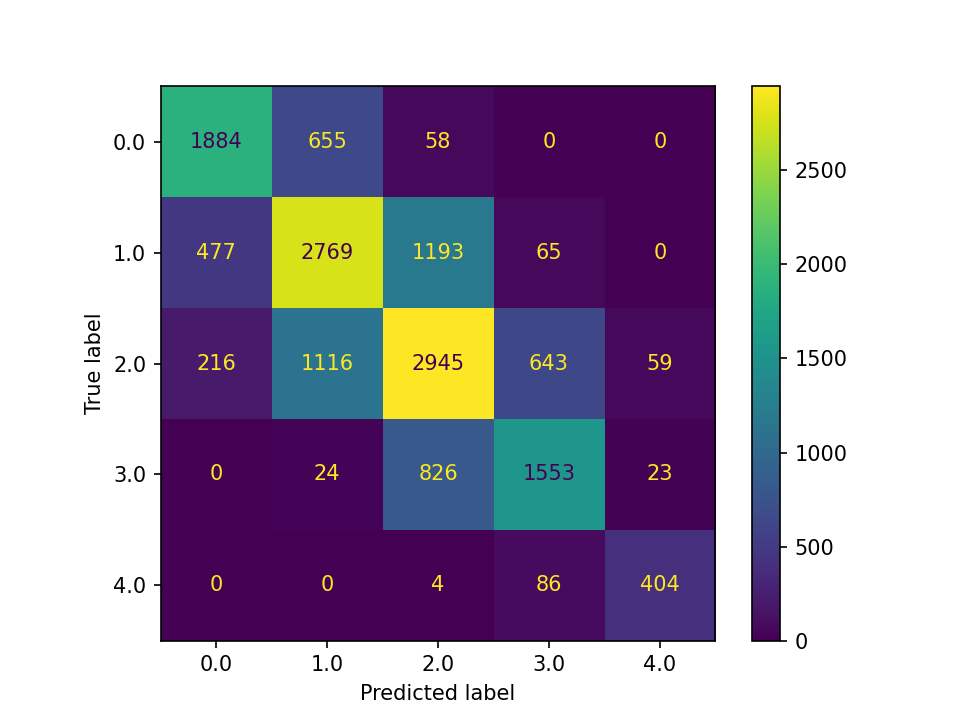
\includegraphics{images/cm_logit_False.png}
\caption{Comparison}
\end{figure}

In the confusion matrix, the rows show the ``True label'' whereas the columns show the ``Predicted label''. All the cells on the diagonal are corrected predicted. Based on the confusion matrix, there are three basic performance metrics: \textbf{accuracy}, \textbf{precision}, and \textbf{recall}. There are also various metrics that are weighted averages. For example, the \textbf{f1 score} is the harmonic mean of precision and recall.

Accuracy is the proportion of individuals that the algorithm has predicted correctly. To calculate the accuracy score, we sum up the values on the diagonal then decide the total:

\[\frac{1884+2769+2945+1553+404}{15000}=0.6370\]

Precision and recall are usually defined based on a certain class. For overall precision and recall scores, we can then take a weighted average. Precision is the proportion of individuals who the algorithm predicted to be a certain class is actually that class. In the above example, 2577 individuals were predicted to be class 0, but only 1884 actually are. As a result, the precision \emph{for class 0} is:

\[\frac{1884}{2577}=0.7311\]

On the other hand, recall is the proportion of individuals who belong to a certain class that the algorithm predicted correctly. IN the above example, 4979 individuals belong to class 2, but only 2945 were predicted correctly by the algorithm. As a result, the recall \emph{for class 2} is:

\[\frac{2945}{4979}=0.5915\]

If we take weighted average of precision and recall of all 5 classes, we get the overall precision and recall scores as 0.6376 and 0.6370, or about 63.7\%.

Economics and social sciences often use the terms ``Type I'' and ``Type II'' errors, which can be related to the discussion here in a binary classification. In a binary classification, we have 4 quadrants:
1. True positive (TP): those who belong to the ``positive'' class and are predicted so;
2. True negative (TN): those who belong to the ``negative'' class and are predicted so. True positive and true negative are on the diagonal;
3. False positive (FP): those who are predicted to be ``positive'' but are actually ``negative';
4. False negative (FN): those who are predicted to be''negative'' but are actually ``positive''.

Type I error corresponds to false positive and Type II error corresponds to false negative.

Before we move on to formally compare results from the 6 algorithms, it is worth noting that random forest, gradient boosting, and XGBoost performed much better than logistic regression in the above simulated data set (with \texttt{random\ seed\ =\ 123}). For example, below is the confusion matrix from XGBoost:

\begin{figure}
\centering
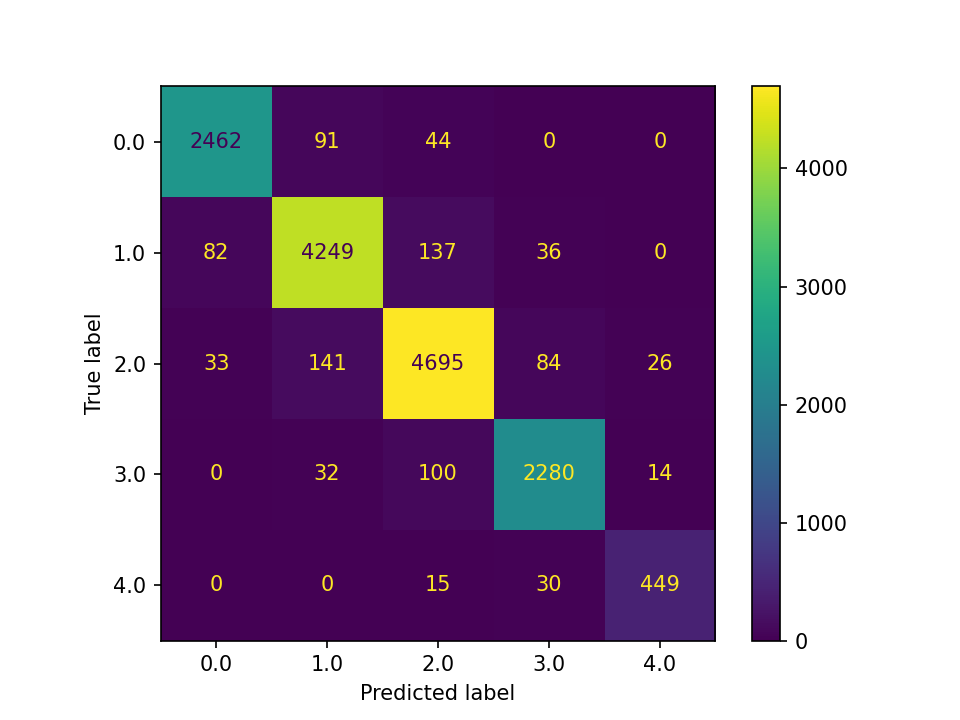
\includegraphics{images/cm_xgboost_False.png}
\caption{Comparison}
\end{figure}

\hypertarget{comparison-the-algorithms}{%
\section{Comparison the Algorithms}\label{comparison-the-algorithms}}

The following \texttt{Python} script runs the comparison between different algorithms for between 6000 and 50000 individuals (sample size):

\begin{Shaded}
\begin{Highlighting}[]
\ImportTok{import}\NormalTok{ matplotlib.pyplot }\ImportTok{as}\NormalTok{ plt}
\ImportTok{import}\NormalTok{ random}
\ImportTok{import}\NormalTok{ pandas }\ImportTok{as}\NormalTok{ pd}
\ImportTok{from}\NormalTok{ multiprocessing }\ImportTok{import}\NormalTok{ Pool, cpu\_count}
\ImportTok{from}\NormalTok{ functools }\ImportTok{import}\NormalTok{ partial}
\ImportTok{from}\NormalTok{ tree\_ensembles }\ImportTok{import}\NormalTok{ run\_tree\_ensembles}

\NormalTok{plt.ion()}

\NormalTok{n\_individuals\_range }\OperatorTok{=} \BuiltInTok{range}\NormalTok{(}\DecValTok{50000}\NormalTok{, }\DecValTok{5999}\NormalTok{, }\OperatorTok{{-}}\DecValTok{2000}\NormalTok{)}


\KeywordTok{def}\NormalTok{ run\_monte\_carlo(n\_individuals\_range, numeric\_only\_bool):}

    \ControlFlowTok{with}\NormalTok{ Pool(}\DecValTok{1}\NormalTok{) }\ImportTok{as}\NormalTok{ pool:}
\NormalTok{        func }\OperatorTok{=}\NormalTok{ partial(run\_tree\_ensembles, }\DecValTok{5}\NormalTok{, }\DecValTok{10}\NormalTok{, }\VariableTok{False}\NormalTok{, }\VariableTok{False}\NormalTok{, numeric\_only\_bool)}
\NormalTok{        results }\OperatorTok{=} \BuiltInTok{list}\NormalTok{(pool.imap(func, n\_individuals\_range))}

    \ControlFlowTok{return}\NormalTok{ results}


\KeywordTok{def}\NormalTok{ plot\_monte\_carlo(data: }\BuiltInTok{list}\NormalTok{):}

\NormalTok{    df\_list }\OperatorTok{=}\NormalTok{ []}
    \ControlFlowTok{for}\NormalTok{ item }\KeywordTok{in}\NormalTok{ data:}
        \ControlFlowTok{for}\NormalTok{ i, inner\_dict }\KeywordTok{in}\NormalTok{ item.items():}
            \ControlFlowTok{for}\NormalTok{ j, inner\_inner\_dict }\KeywordTok{in}\NormalTok{ inner\_dict.items():}
\NormalTok{                value }\OperatorTok{=}\NormalTok{ inner\_inner\_dict[}\StringTok{\textquotesingle{}cv\_score\textquotesingle{}}\NormalTok{]}
\NormalTok{                df\_list.append(\{}\StringTok{\textquotesingle{}i\textquotesingle{}}\NormalTok{: i, }\StringTok{\textquotesingle{}Model\textquotesingle{}}\NormalTok{: j, }\StringTok{\textquotesingle{}cv\_score\textquotesingle{}}\NormalTok{: value\})}

\NormalTok{    df }\OperatorTok{=}\NormalTok{ pd.DataFrame(df\_list)}

\NormalTok{    fig, ax }\OperatorTok{=}\NormalTok{ plt.subplots()}

\NormalTok{    num\_models }\OperatorTok{=} \BuiltInTok{len}\NormalTok{(df[}\StringTok{\textquotesingle{}Model\textquotesingle{}}\NormalTok{].unique())}
\NormalTok{    cmap }\OperatorTok{=}\NormalTok{ plt.get\_cmap(}\StringTok{\textquotesingle{}Set2\textquotesingle{}}\NormalTok{)  }\CommentTok{\# Use the Set2 color map}

    \ControlFlowTok{for}\NormalTok{ i, model }\KeywordTok{in} \BuiltInTok{enumerate}\NormalTok{(df[}\StringTok{\textquotesingle{}Model\textquotesingle{}}\NormalTok{].unique()):}
\NormalTok{        model\_data }\OperatorTok{=}\NormalTok{ df[df[}\StringTok{\textquotesingle{}Model\textquotesingle{}}\NormalTok{] }\OperatorTok{==}\NormalTok{ model]}
\NormalTok{        color }\OperatorTok{=}\NormalTok{ cmap(i }\OperatorTok{\%}\NormalTok{ num\_models)  }\CommentTok{\# Cycle through the color map}
\NormalTok{        ax.plot(model\_data[}\StringTok{\textquotesingle{}i\textquotesingle{}}\NormalTok{], model\_data[}\StringTok{\textquotesingle{}cv\_score\textquotesingle{}}\NormalTok{], }\StringTok{\textquotesingle{}{-}o\textquotesingle{}}\NormalTok{, c}\OperatorTok{=}\NormalTok{color, label}\OperatorTok{=}\NormalTok{model, alpha}\OperatorTok{=}\FloatTok{0.5}\NormalTok{)}

\NormalTok{    ax.set\_xlabel(}\StringTok{\textquotesingle{}Number of Individuals\textquotesingle{}}\NormalTok{)}
\NormalTok{    ax.set\_ylabel(}\StringTok{\textquotesingle{}Cross Validation Scores\textquotesingle{}}\NormalTok{)}
\NormalTok{    ax.set\_title(}\StringTok{\textquotesingle{}Plot of Cross Validation Scores\textquotesingle{}}\NormalTok{)}
\NormalTok{    ax.legend([}\StringTok{\textquotesingle{}Logit\textquotesingle{}}\NormalTok{, }\StringTok{\textquotesingle{}Decision Tree\textquotesingle{}}\NormalTok{, }\StringTok{\textquotesingle{}Random Forest\textquotesingle{}}\NormalTok{, }\StringTok{\textquotesingle{}Adaboost\textquotesingle{}}\NormalTok{, }\StringTok{\textquotesingle{}GBM\textquotesingle{}}\NormalTok{, }\StringTok{\textquotesingle{}XGBoost\textquotesingle{}}\NormalTok{],}
\NormalTok{              loc}\OperatorTok{=}\StringTok{\textquotesingle{}lower right\textquotesingle{}}\NormalTok{,}
\NormalTok{              fontsize}\OperatorTok{=}\DecValTok{9}\NormalTok{, markerscale}\OperatorTok{=}\FloatTok{1.5}\NormalTok{, scatterpoints}\OperatorTok{=}\DecValTok{1}\NormalTok{,}
\NormalTok{              fancybox}\OperatorTok{=}\VariableTok{True}\NormalTok{, framealpha}\OperatorTok{=}\FloatTok{0.5}\NormalTok{)}
\end{Highlighting}
\end{Shaded}

The script intends to use parallel computing, but algorithms in \texttt{scikit-learn} already utilized parallel computing, we set \texttt{Pool(1)} at the end to run it with single thread. Two comparisons, with and without using the categorical features in generating the target groups, are run. The average score from 10-fold cross validations are recorded and plotted. Here is the result from when \texttt{kmeans} generated the target groups without using the categorical columns (but they are still in the training data):

\begin{figure}
\centering
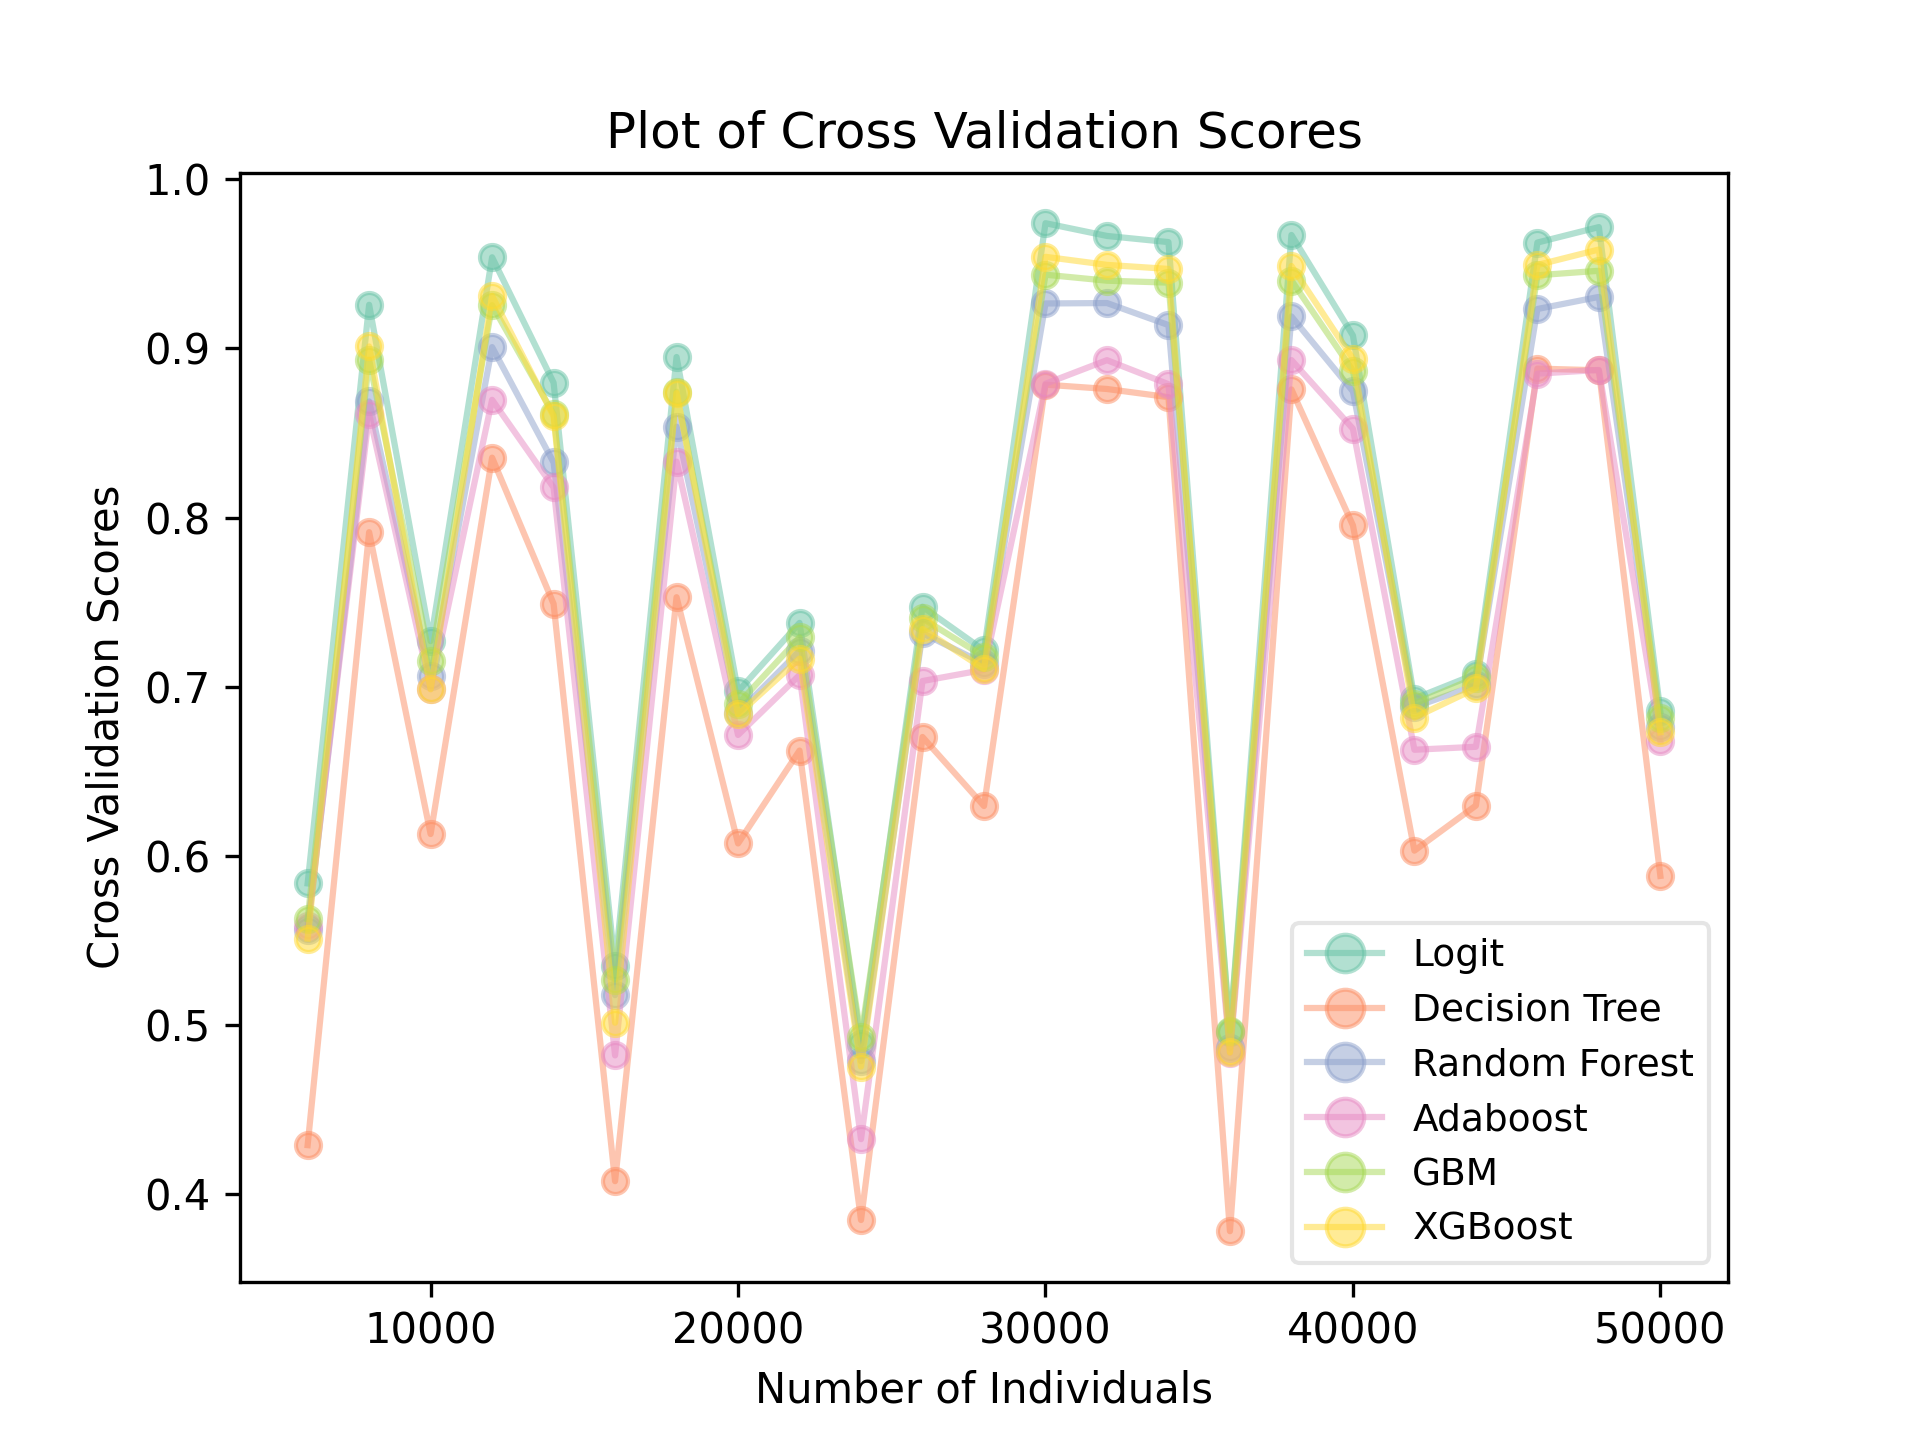
\includegraphics{images/comparison_true.png}
\caption{Comparison}
\end{figure}

A single decision tree performed the worst, while, surprisingly, logistic regression performed the best. Keep in mind that the ups and downs at different sample sizes do not indicate that more data is worse. There is some random components in how the data was generated, namely with \texttt{kmeans} algorithm.

When categorical columns are included in generating the target groups, there exists more variations among algorithms:

\begin{figure}
\centering
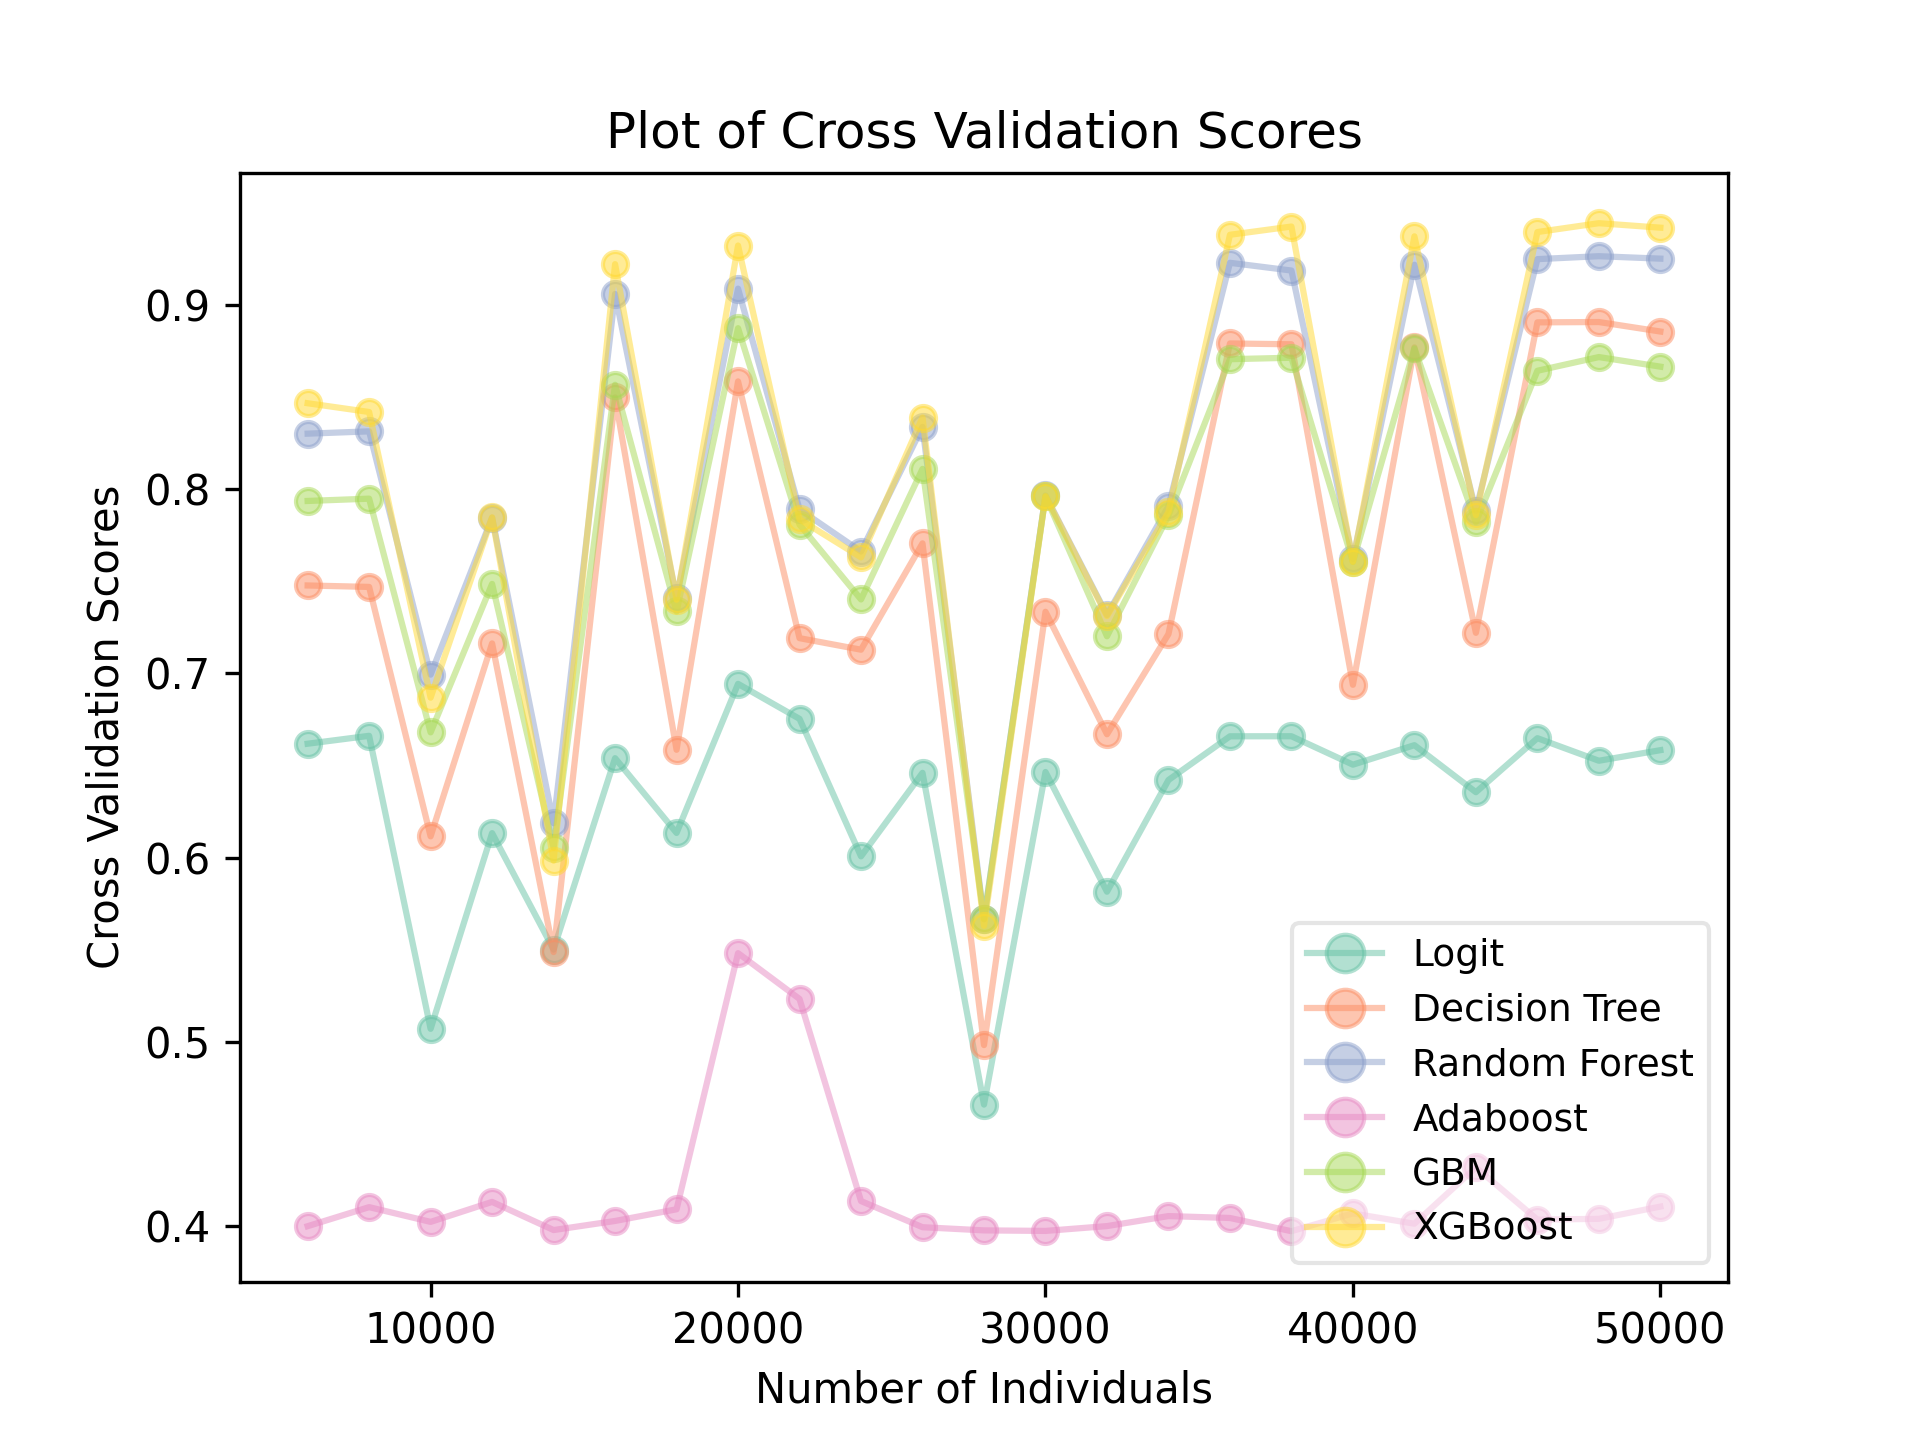
\includegraphics{images/comparison_false.png}
\caption{Comparison}
\end{figure}

In here, \texttt{Adaboost} performed noticeably worse than all other algorithms. Logistic regression also fell, partly because its inability to deal with categorical features (even with one-hot encoding). Not surprisingly, the performances of \texttt{Random\ Forest}, \texttt{Gradient\ Boosting}, and \texttt{XGBoost} remain strong.

\hypertarget{summary}{%
\section{Summary}\label{summary}}

In this chapter, we have covered the decision tree algorithm as well as bagging and boosting algorithms based on decision tree. There are few important takeaways and remarks.

First, ensemble methods is a general method that applies to algorithms beyond tree-based models. You could easily applied the same principle of bagging and boosting on regression models. For example, you can build several regressors with a bootstrap data set, or include only some of the features, or use weighted methods to boost. As a matter of fact, ensemble can also be built between regression and classification algorithms. Gradient Boosting and XGBoost can actually be considered as such ensemble: while the end-goal of the algorithms were to predict classes, at their core, they are regressions.

Second, tree-based models can be used for regression problems. For example, instead of \texttt{RandomForestClassifier}, you can use \texttt{RandomForestRegressor} for a regression problem. When you are using a classification algorithm on a continuous target. Instead of trying to predict classes, the \texttt{RandomForestRegressor}, as well as other classification used for regression problems, aims to predict the mean of the target. We will cover this in more depth in a later chapter.

Third, in general, it is more accurate to predict classes than continuous values. Due to this, the use of classification algorithms may be broader than most expected. For example, it is possible to convert a regression problem (in predicting continuous quantities) to classification problems. The market share example given in the beginning of the chapter is a good example. Another example is e-commerce. Most e-commerce owners have a limited offering. As a result, instead of predicting the sales per month or the dollar value of a customer, it is easier to predict whether and how many a customer would buy. This method can be especially powerful since a business owner often has control over the price of the products.

Lastly, tree-based methods can be used for causal inference. While causal inference itself is a topic of a later chapter, for readers who are familiar with causal inference methods, you can easily find parallel between decision tree and propensity score matching (PSM): individuals who ended up in the same leave have something in common, and hence can provide good matching samples. This is the basic idea behind \texttt{causal\ tree} (Athey and Imbens, 2016).

\hypertarget{references-1}{%
\section{References}\label{references-1}}

\begin{itemize}
\tightlist
\item
  S. Athey and G. Imbens, ``Recursive partitioning for heterogeneous causal effects'', \emph{PNAS}, 2016.
\item
  L. Breiman, ``Bagging predictors'', \emph{Machine Learning}, 1996.
\item
  L. Breiman, ``Pasting small votes for classification in large databases and on-line'', \emph{Machine Learning}, 1999.
\item
  L. Breiman, ``Random forest'', \emph{Machine Learning}, 2001.
\item
  Y. Freund and R. Schapire, ``A Decision-Theoretic Generalization of on-Line Learning and an Application to Boosting'', 1995.
\item
  J. Friedman, ``Greedy Function Approximation: A Gradient Boosting Machine'', \emph{The Annals of Statistics}, 2001.
\item
  T. Ho, ``The random subspace method for constructing decision forests'', \emph{Pattern Analysis and Machine Intelligence}, 1998.
\item
  G. Louppe and P. Geurts, ``Ensembles on Random Patches'', \emph{Machine Learning and Knowledge Discovery in Databases}, 2012.
\item
  \url{https://scikit-learn.org/stable/modules/tree.html}
\item
  \url{https://xgboost.readthedocs.io/en/stable/tutorials/model.html}
\item
  \url{https://machinelearningmastery.com/boosting-and-adaboost-for-machine-learning/}
\item
  \url{https://stats.stackexchange.com/questions/157870/scikit-binomial-deviance-loss-function}
\item
  \url{https://www.ccs.neu.edu/home/vip/teach/MLcourse/4_boosting/slides/}
\end{itemize}

\hypertarget{parts}{%
\chapter{Parts}\label{parts}}

You can add parts to organize one or more book chapters together. Parts can be inserted at the top of an .Rmd file, before the first-level chapter heading in that same file.

Add a numbered part: \texttt{\#\ (PART)\ Act\ one\ \{-\}} (followed by \texttt{\#\ A\ chapter})

Add an unnumbered part: \texttt{\#\ (PART\textbackslash{}*)\ Act\ one\ \{-\}} (followed by \texttt{\#\ A\ chapter})

Add an appendix as a special kind of un-numbered part: \texttt{\#\ (APPENDIX)\ Other\ stuff\ \{-\}} (followed by \texttt{\#\ A\ chapter}). Chapters in an appendix are prepended with letters instead of numbers.

\hypertarget{footnotes-and-citations}{%
\chapter{Footnotes and citations}\label{footnotes-and-citations}}

\hypertarget{footnotes}{%
\section{Footnotes}\label{footnotes}}

Footnotes are put inside the square brackets after a caret \texttt{\^{}{[}{]}}. Like this one \footnote{This is a footnote.}.

\hypertarget{citations}{%
\section{Citations}\label{citations}}

Reference items in your bibliography file(s) using \texttt{@key}.

For example, we are using the \textbf{bookdown} package \citep{R-bookdown} (check out the last code chunk in index.Rmd to see how this citation key was added) in this sample book, which was built on top of R Markdown and \textbf{knitr} \citep{xie2015} (this citation was added manually in an external file book.bib).
Note that the \texttt{.bib} files need to be listed in the index.Rmd with the YAML \texttt{bibliography} key.

The RStudio Visual Markdown Editor can also make it easier to insert citations: \url{https://rstudio.github.io/visual-markdown-editing/\#/citations}

\hypertarget{blocks}{%
\chapter{Blocks}\label{blocks}}

\hypertarget{equations}{%
\section{Equations}\label{equations}}

Here is an equation.

\begin{equation} 
  f\left(k\right) = \binom{n}{k} p^k\left(1-p\right)^{n-k}
  \label{eq:binom}
\end{equation}

You may refer to using \texttt{\textbackslash{}@ref(eq:binom)}, like see Equation \eqref{eq:binom}.

\hypertarget{theorems-and-proofs}{%
\section{Theorems and proofs}\label{theorems-and-proofs}}

Labeled theorems can be referenced in text using \texttt{\textbackslash{}@ref(thm:tri)}, for example, check out this smart theorem \ref{thm:tri}.

\begin{theorem}
\protect\hypertarget{thm:tri}{}\label{thm:tri}For a right triangle, if \(c\) denotes the \emph{length} of the hypotenuse
and \(a\) and \(b\) denote the lengths of the \textbf{other} two sides, we have
\[a^2 + b^2 = c^2\]
\end{theorem}

Read more here \url{https://bookdown.org/yihui/bookdown/markdown-extensions-by-bookdown.html}.

\hypertarget{callout-blocks}{%
\section{Callout blocks}\label{callout-blocks}}

The R Markdown Cookbook provides more help on how to use custom blocks to design your own callouts: \url{https://bookdown.org/yihui/rmarkdown-cookbook/custom-blocks.html}

\hypertarget{sharing-your-book}{%
\chapter{Sharing your book}\label{sharing-your-book}}

\hypertarget{publishing}{%
\section{Publishing}\label{publishing}}

HTML books can be published online, see: \url{https://bookdown.org/yihui/bookdown/publishing.html}

\hypertarget{pages}{%
\section{404 pages}\label{pages}}

By default, users will be directed to a 404 page if they try to access a webpage that cannot be found. If you'd like to customize your 404 page instead of using the default, you may add either a \texttt{\_404.Rmd} or \texttt{\_404.md} file to your project root and use code and/or Markdown syntax.

\hypertarget{metadata-for-sharing}{%
\section{Metadata for sharing}\label{metadata-for-sharing}}

Bookdown HTML books will provide HTML metadata for social sharing on platforms like Twitter, Facebook, and LinkedIn, using information you provide in the \texttt{index.Rmd} YAML. To setup, set the \texttt{url} for your book and the path to your \texttt{cover-image} file. Your book's \texttt{title} and \texttt{description} are also used.

This \texttt{gitbook} uses the same social sharing data across all chapters in your book- all links shared will look the same.

Specify your book's source repository on GitHub using the \texttt{edit} key under the configuration options in the \texttt{\_output.yml} file, which allows users to suggest an edit by linking to a chapter's source file.

Read more about the features of this output format here:

\url{https://pkgs.rstudio.com/bookdown/reference/gitbook.html}

Or use:

\end{document}
